% The contents of this file is 
% Copyright (c) 2009-2011  Charles R. Severance, All Righs Reserved
% Copyright (c) 2009-2011  Charles R. Severance, All Righs Reserved

%\documentclass[10pt,b5paper]{book}
\documentclass[11pt]{book}
% \usepackage[width=5.25in,height=7.50in,hmarginratio=3:2,vmarginratio=1:1]{geometry}
\usepackage[size=journal,gutter=0.75in,trim,bleed]{createspace}

\usepackage{pslatex}
\usepackage{url}
\usepackage{fancyhdr}
\usepackage{graphicx}
\usepackage{amsmath, amsthm, amssymb}
\usepackage{exercise}
\usepackage{makeidx}
\usepackage{setspace}
\usepackage{hevea}
\usepackage{alltt}
\usepackage{upquote}
\usepackage[hangul]{kotex}
%\kscntformat{chapter}{}{~장}
\usepackage[T1]{fontenc}
\usepackage[utf8]{inputenc}

 
%\newcommand{\thetitle}{Python for Informatics: Exploring Information}
\newcommand{\thetitle}{정보교육을 위한 파이썬}
\newcommand{\thesubtitle}{정보탐색을 통한 데이터 과학자로의 여정}
\newcommand{\theversion}{0.0.9-d2}
\newcommand{\theauthor}{Charles R. Severance, 번역: 이광춘}

\author{Charles R. Severance, 번역: 이광춘}
%\author{번역: 이광춘}

\makeindex

\begin{document}

\frontmatter

\input{00-cover}
\input{00-preface}

% START THE BOOK
\mainmatter

\input{01-intro}
% LaTeX source for ``Python for Informatics: Exploring Information''
% Copyright (c)  2010-  Charles R. Severance, All Rights Reserved
% 한국어 번역 : 이광춘, 한정수
\chapter{변수, 표현식, 문장(Statement)}

\section{값(Value)과 자료형(Type)}
\index{값(value)}
\index{자료형(type)}
\index{문자열(string)}

{\bf 값(Value)}은 문자와 숫자처럼 프로그램이 다루는 가장 기본이 되는 단위이다. 
지금까지 살펴본 값은 {\tt 1}, {\tt 2} 그리고 \verb"'Hello,World!'" 이다.

상기 값은 다른 {\bf 자료형(Type)}에 속하는데, {\tt 2}는 정수, \verb" 'Hello,World!'" 는 
{\bf 문자열(String)}에 속하는데, 문자(Letter)를 일련의 열(sequence)의 형태로 되어 있어서 문자열이라고 부른다. 
인용부호에 감싸여 있어서, 여러분과 인터프리터는 문자열을 식별할 수 있다. 

{\tt print } 문은 정수에도 사용할 수 있다. {\tt python} 명령어를 실행하여 인터프리터를 구동시키자.

\index{quotation mark}

\beforeverb
\begin{verbatim}
python
>>> print 4
4
\end{verbatim}
\afterverb
%
값이 어떤 형인지 확신을 못한다면, 인터프리터가 알려준다.

\beforeverb
\begin{verbatim}
>>> type('Hello, World!')
<type 'str'>
>>> type(17)
<type 'int'>
\end{verbatim}
\afterverb
%

놀랍지도 않게, strings은 {\tt str} 형식이고, 정수는 {\tt int} 형식이다. 
다소 명백하지는 않지만, 소숫점을 가진 숫자는 {\tt float} 형식이다. 왜냐하면 이들 숫자가 {\bf 부동소수점} 형식으로 표현되기 때문이다.

\index{자료형 (type)}
\index{문자열 자료형 (string type)}
\index{자료형(type)!문자열 자료형 (str)}
\index{정수형 (int type)}
\index{자료형(type)!int (정수형)}
\index{부동소수점형 (float type)}
\index{자료형(type)!float (부동소수점형)}

\beforeverb
\begin{verbatim}
>>> type(3.2)
<type 'float'>
\end{verbatim}
\afterverb
%

\verb"'17'", \verb"'3.2'" 같은 값은 어떨가? 숫자처럼 보이지만 문자열처럼 인용부호에 감싸여 있다.

\index{인용 부호 (quotation mark)}

\beforeverb
\begin{verbatim}
>>> type('17')
<type 'str'>
>>> type('3.2')
<type 'str'>
\end{verbatim}
\afterverb
%

\verb"'17'", \verb"'3.2'" 은 문자열이다.

{\tt 1,000,000} 처럼 아주 큰 정수를 입력할 때, 세자리 숫자마다 콤마(,)를 사용하고 싶을 것이다. 하지만, 파이썬에서 적법하게 정수를 표현하는 것은 아니지만 문법적으로는 적합하다.

\beforeverb
\begin{verbatim}
>>> print 1,000,000
1 0 0
\end{verbatim}
\afterverb
%

하지만, 파이썬 실행 결과는 우리가 기대했던 것이 아니다. 파이썬에서는 {\tt 1,000,000} 을 콤마(',')로 구분된 정수로 인식한다. 따라서 사이 사이 공백을 넣어 출력했다.

\index{의미론적 오류 (semantic error)} % \index{semantic error}
\index{error (오류)!semantic (의미론)} % \index{error!semantic}
\index{error message (오류 메시지)}

이 사례가 여러분이 처음 경험하게 되는 의미론적 오류(semantic error)다. 
코드가 에러 메세지 없이 실행이되지만, ''올바른(right)'' 작동을 하는 것은 아니다.

\section{변수(Variable)}
\index{변수 (variable)} % \index{variable}
\index{대입문 (assignment statement)} %\index{assignment statement}
\index{statement (문장)!assignment (대입)} % \index{statement!assignment}

프로그래밍 언어의 가장 강력한 기능 중의 하나는 변수를 다룰 수 있는 능력이다. {\bf 변수(Variable)}는 값을 참조하는 이름이다.

{\bf 대입문(Assignment statement)}는 새로운 변수를 생성하고 값을 변수에 대입한다.

\beforeverb
\begin{verbatim}
>>> message = 'And now for something completely different'
>>> n = 17
>>> pi = 3.1415926535897931
\end{verbatim}
\afterverb
%

상기 예제는 세가지 대입 사례를 보여준다. 첫 번째 대입 예제는 {\tt message} 변수에 문자열을 대입한다. 두 번째 예제는 변수 {\tt n}에 정수 {\tt 17}을 대입한다. 세 번째 예제는 {\tt pi}변수에 $\pi$ 근사값을 대입한다.

변수 값을 출력하기 위해서 {\tt print}문을 사용한다.

\beforeverb
\begin{verbatim}
>>> print n
17
>>> print pi
3.14159265359
\end{verbatim}
\afterverb
%

변수 자료형(type)은 변수가 참조하는 값의 자료형이다.

\beforeverb
\begin{verbatim}
>>> type(message)
<type 'str'>
>>> type(n)
<type 'int'>
>>> type(pi)
<type 'float'>
\end{verbatim}
\afterverb
%

\section{변수명(Variable name)과 예약어(keywords)}
\index{keyword (예약어)} % \index{keyword}

대체로 프로그래머는 의미있는 변수명을 고른다. 프로그래머는 변수가 사용되는 것에 대해 문서화도 한다.

변수명은 임의로 길 수 있다. 변수명은 문자와 숫자를 포함할 수 있지만, 문자로 변수명을 시작해야 한다. 첫 변수명을 대문자로 사용해도 되지만 소문자로 변수명을 시작하는 것도 좋은 생각이다. (후에 왜 그런지 보게 될 것이다.)

변수명에 밑줄(underscore character, \verb"_")이 들어갈 수 있다. 종종 \verb"my_name" 혹은 \verb"airspeed_of_unladen_swallow" 처럼 밑줄은 여러 단어와 함께 사용된다.
변수명을 밑줄로 시작해서 작성할 수 있지만, 다른 사용자가 사용할 라이브러리를 작성하는 경우가 아니라면, 일반적으로 밑줄로 시작하는 변수명은 피한다.

\index{밑줄 (underscore character)} % \index{underscore character}

변수명을 적합하게 작성하지 못하다면, 구문 오류가 발생한다.

\beforeverb
\begin{verbatim}
>>> 76trombones = 'big parade'
SyntaxError: invalid syntax
>>> more@ = 1000000
SyntaxError: invalid syntax
>>> class = 'Advanced Theoretical Zymurgy'
SyntaxError: invalid syntax
\end{verbatim}
\afterverb
%

{\tt 76trombones} 변수명은 문자로 시작하지 않아서 적합하지 않다. 
{\tt more@}은 특수 문자 ({\tt @})를 변수명에 포함해서 적합하지 않다. 
하지만, {\tt class} 변수명은 뭐가 잘못된 것일까?

구문 오류 이유는 {\tt class}가 파이썬의 예약어 중의 하나라고 밝혀졌다. 
인터프리터가 예약어를 사용하여 프로그램 구조를 파악하기 위해서 사용하지만, 변수명으로는 사용할 수 없다.

\index{예약어 (keyword)}
%\index{keyword}

파이썬에는 31개 키워드\footnote{Python 3.0 에서 {\tt exec} 은 더 이상 예약어가 아니지만, {\tt nonlocal} 은 여전히 예약어다.}가 예약어로 이미 사용중에 있다.

\beforeverb
\begin{verbatim}
and       del       from      not       while    
as        elif      global    or        with     
assert    else      if        pass      yield    
break     except    import    print              
class     exec      in        raise              
continue  finally   is        return             
def       for       lambda    try
\end{verbatim}
\afterverb
%

상기 예약어 목록을 주머니에 넣고 잘 가지고 다니고 싶을 것이다. 
만약 인터프리터가 변수명 중 하나에 대해 불평을 하지만 이유를 모르는 경우, 예약어 목록에 변수명이 있는지 확인해 보세요.

\section{문장(Statement)}

{\bf 문장(statement)}은 파이썬 인터프리터가 실행하는 코드 단위다. 지금까지 print, assignment 두 종류의 문장을 살펴봤습니다.

\index{문장 (statement)}
\index{인터랙티브 모드 (interactive mode)}
\index{스크립트 모드 (script mode)}
%\index{statement}
%\index{interactive mode}
%\index{script mode}

인터랙트브 모드에서 문장을 입력하면, 인터프리터는 문장을 실행하고, 만약 출력할 것이 있다면 결과를 화면에 출력합니다.

스크립트는 보통 여러줄의 문장으로 구성됩니다. 하나 이상의 문장이 있다면, 스트테이트먼트가 실행되며서 결과가 한번에 하나씩 나타납니다.

예를 들어, 다음의 스크립트를 생각해 봅시다.

\beforeverb
\begin{verbatim}
print 1
x = 2
print x
\end{verbatim}
\afterverb
%

상기 스크립트는 다음 결과를 출력합니다.

\beforeverb
\begin{verbatim}
1
2
\end{verbatim}
\afterverb
%

대입 문장{\tt (x=2)}은 결과를 출력하지 않습니다.

\section{연산자(Operator)와 피연산자(Operands)}
\index{연산자 (operator), 산술(arithmetic)}
\index{산술 연산자 (arithmetic operator)}
\index{피연산자 (operand)}
\index{표현식 (expression)}

%\index{operator, arithmetic}
%\index{arithmetic operator}
%\index{operand}
%\index{expression}

{\bf 연산자(Operators)}는 덧셈, 곱셈 같은 계산(Computation)을 표현하는 특별한 기호입니다. 연산가자 적용되는 값을 {\bf 피연산자(operands)}라고 합니다.

다음의 예제에서 보듯이, {\tt +}, {\tt -}, {\tt *}, {\tt /}, {\tt **} 연산자는 덧셈, 뺄셈, 곱셈, 나눗셈, 지수승을 수행합니다.

\beforeverb
\begin{verbatim}
20+32   hour-1   hour*60+minute   minute/60   5**2   (5+9)*(15-7)
\end{verbatim}
\afterverb
%
나눗셈 연산자는 여러분이 기대하는 것을 수행하지 않을 수도 있습니다.

\beforeverb
\begin{verbatim}
>>> minute = 59
>>> minute/60
0
\end{verbatim}
\afterverb
%

{\tt minute} 값은 59, 보통 59를 60으로 나누면 0 대신에 0.98333 입니다. 이런 차이가 발생하는 이유는 파이썬이 {\bf 소수점 이하 버림 나눗셈}\footnote{파이썬 3.0 에서 이 나눗셈 값은 {\tt 소수점}입니다. 파이썬 3.0 에 도입된 새로운 연산자{\tt //}는 정수형 나눗셈을 수행합니다.}을 하기 때문입니다.

\index{파이썬 3.0 (Python 3.0)}
\index{버림 나눗셈 (floor division)}
\index{부동 소수점 나눗셈 (floating-point division)}
\index{나눗셈 (division)!절사 (floor)}
\index{나눗셈 (division)!부동 소수점 (floating-point)}
%\index{Python 3.0}
%\index{floor division}
%\index{floating-point division}
%\index{division!floor}
%\index{division!floating-point}

두 개의 피연산자가 정수이면, 결과도 정수입니다. 부동 소수점 나눗셈은 소수점 이하를 절사합니다.
그래서 예제에서 소수점 이하 잘라버려 0 이 됩니다.

만약 두 개의 피연산자 중 하나가 부동 소수점 수이면, 파이썬은 부동 소수점 나눗셈을 수행하고 결과는 {\tt 부동 소수점형} 값이 된다.

\beforeverb
\begin{verbatim}
>>> minute/60.0
0.98333333333333328
\end{verbatim}
\afterverb

\section{표현식(Expression)}

{\bf 표현식 (expression)}은 값, 변수, 연산자 조합니다. 값은 자체로 표현식이고, 변수도 동일하다. 따라서 다음 표현식은 모두 적합하다. 
(변수 {\tt x}는 사전에 어떤 값이 대입되었다고 가정한다.)

%\index{expression}
%\index{evaluate}
\index{표현식 (expression)}
\index{평가 (evaluate)}

\beforeverb
\begin{verbatim}
17
x
x + 17
\end{verbatim}
\afterverb
%

인터랙티브 모드에서 표현식을 입력하면, 인터프리터는 표현식을 {\bf 평가(evaluate)}하고 값을 표시한다.

\beforeverb
\begin{verbatim}
>>> 1 + 1
2
\end{verbatim}
\afterverb
%

하지만, 스크립트에서는 표현식 자체로 어떠한 것도 수행하지는 않는다. 초심자에게 혼란스러운 점이다.

\begin{ex}

파이썬 인터프리터에 다음 문장을 입력하고 결과를 보세요.

\beforeverb
\begin{verbatim}
5
x = 5
x + 1
\end{verbatim}
\afterverb
%
\end{ex}


\section{연산자 적용 우선순위 (Order of Operations)}
\index{연산자 적용 우선순위 (order of operations)}
\index{우선순위 규칙 (rules of precedence)}
\index{PEMDAS}
%\index{order of operations}
%\index{rules of precedence}
%\index{PEMDAS}

1개 이상의 연산자가 표현식에 등장할 때, 
연산자 평가 순서는 {\bf  우선순위 규칙(rules of precedence)}에 따른다. 
수학 연산자에 대해서 파이썬은 수학적 관례를 동일하게 따른다. 영어 두문어 {\bf PEMDAS}는 기억하기 좋은 방식이다.

\index{괄호 (parentheses)!최우선 우선순위 (overriding precedence)}
%\index{parentheses!overriding precedence}

\begin{itemize}

\item {\bf 괄호(Parentheses)}는 가장 높은 순위를 가지고 여러분이 원하는 순위에 맞춰 실행할 때 사용한다. 
괄호내의 식이 먼저 실행되기 때문에 {\tt 2 * (3-1)} 은 4가 정답이고, {\tt (1+1)**(5-2)}는 8이다. 
괄호를 사용하여 표현식을 좀더 읽기 쉽게 하려고 사용하기도 한다. 
{\tt (minute * 100) / 60} 는 실행순서가 결과값에 영향을 주지 않지만 가독성이 상대적으로 더 좋다.

\item {\bf 지수승(Exponentiation)}이 다음으로 높은 우선순위를 가진다. 
그래서 {\tt 2**1+1}는 4가 아니라 3이고, {\tt 3*1**3}는 27이 아니고 3이다. 

\item {\bf 곱셈(Multiplication)과 나눗셈(Division)}은 동일한 우선순위를 가지지만, 덧셈(Addition), 뺄셈(Substraction)보다 높은 우선 순위를 가진다. 덧셈과 뺄샘은 같은 실행 우선순위를 갖는다. {\tt 2*3-1}는 4가 아니고 5이고, {\tt 6+4/2}는 5가 아니라 8이다.

\item 같은 실행 순위를 갖는 연산자는 왼쪽에서부터 오른쪽으로 실행된다. 
{\tt 5-3-1} 표현식은 3이 아니고 1이다. 왜냐하면 {\tt 5-3}이 먼저 실행되고 나서 {\tt 2}에서 {\tt 1}을 빼기 때문이다.

\end{itemize}

여러분이 의도한 순서대로 연산이 수행될 수 있도록, 좀 의심스러운 경우는 항상 괄호를 사용한다.

\section{나머지 연산자 (Modulus Operator)}

%\index{modulus operator}
%\index{operator!modulus}
\index{나머지 연산자 (modulus operator)}
\index{연산자 (operator)!나머지 (modulus)}

{\bf 나머지 연산자(modulus operator)}는 정수에 사용하며, 첫번째 피연산자를 두번째 피연산자가 나눌 때 나머지 값이 생성된다. 
파이썬에서 나머지 연산자는 퍼센트 기호(\verb"%")다. 구문은 다른 연산자와 동일하다.

\beforeverb
\begin{verbatim}
>>> quotient = 7 / 3
>>> print quotient
2
>>> remainder = 7 % 3
>>> print remainder
1
\end{verbatim}
\afterverb
%

7을 3으로 나누면 몫이 2가 되고 나머지가 1이 된다.

나머지 연산자가 놀랍도록 유용다다. 예를 들어 한 숫자를 다른 숫자로 나눌 수 있는지 없는지를 확인할 수도 있다. 
{\tt x \% y} 값이 0 이라면, {\tt x}를 {\tt y}로 나눌 수 있다.

%\index{divisibility}
\index{가분성 (divisibility)}

또한, 숫자에서 가장 오른쪽 숫자를 분리하는데도 사용된다. 
예를 들어 {\tt x \% 10} 은 {\tt x}가 10진수인 경우 가장 오른쪽 숫자를 뽑아낼 수 있고, 동일한 방식으로 {\tt x \% 100}은 가장 오른쪽 2개 숫자를 뽑아낼 수도 있다.

\section{문자열 연산자 (String Operator)}
\index{string (문자열)!operation (연산)}
\index{operator (연산자)!string (문자열)}
%\index{string!operation}
%\index{operator!string}

{\tt +} 연산자는 문자열에도 동작하지만, 수학에서 말하는 덧셈은 아니다. 
대신에 문자열 끝과 끝을 붙이는 {\bf 연결(concatenation)} 작업을 수행한다. 예를 들어,

\index{연결 (concatenation)}
%\index{concatenation}

\beforeverb
\begin{verbatim}
>>> first = 10
>>> second = 15
>>> print first+second
25
>>> first = '100'
>>> second = '150'
>>> print first + second
100150
\end{verbatim}
\afterverb
%

상기 프로그램 출력은 {\tt 100150} 이다.

\section{사용자에게서 입력값 받기}

\index{키보드 입력 (keyboard input)}
%\index{keyboard input}

때때로 키보드를 통해서 사용자로부터 변수에 대한 값을 입력받고 싶을 때가 있다. 
키보드\footnote{파이썬 3.0에서 입력 함수는 {\tt input}으로 명명되었다.}로부터 입력값을 받는 \verb"raw_input" 이라는 내장(built-in) 함수를 파이썬에서 제공한다. 입력 함수가 호출되면, 파이썬은 실행을 멈추고 사용자가 무언가 입력하기를 기다린다. 
사용자가 {\sf Return (리턴)} 혹은 {\sf Enter (엔터)} 키를 누르게 되면 프로그램이 다시 실행되고, \verb"raw_input"은 사용자가 입력한 것을 문자열로 반환한다.

\index{파이썬 3.0 (Python 3.0)}
\index{raw\_input 함수 (raw\_input function)}
\index{함수 (function)!raw\_input}
%\index{Python 3.0}
%\index{raw\_input function}
%\index{function!raw\_input}

\beforeverb
\begin{verbatim}
>>> input = raw_input()
Some silly stuff
>>> print input
Some silly stuff
\end{verbatim}
\afterverb
%

사용자로부터 입력 받기 전에 프롬프트에서 사용자가 어떤 값을 입력해야 하는지 정보를 제공하는 것도 좋은 생각이다. 
입력을 받기 위해 잠시 멈춰있을 때, 사용자에게 표시되도록 \verb"raw_input" 함수에 문자열을 전달할 수 있다.

\index{프롬프트 (prompt)}
%\index{prompt}

\beforeverb
\begin{verbatim}
>>> name = raw_input('What is your name?\n')
What is your name?
Chuck
>>> print name
Chuck
\end{verbatim}
\afterverb
%

프롬프트의 끝에 \verb"\n" 은 {\bf 개행(newline)}을 의미한다. 개행은 줄을 바꾸게 하는 특수 문자다. 
이런 이유 때문에 사용자 입력이 프롬프트 밑에 출력된다.

\index{개행 (newline)}

만약 사용자가 정수를 입력하기를 바란다면, 
{\tt int()}함수를 사용하여 반환되는 값을 {\tt 정수(int)}로 자료형을 변환한다.

\beforeverb
\begin{verbatim}
>>> prompt = 'What...is the airspeed velocity of an unladen swallow?\n'
>>> speed = raw_input(prompt)
What...is the airspeed velocity of an unladen swallow?
17
>>> int(speed)
17
>>> int(speed) + 5
22
\end{verbatim}
\afterverb
%

하지만, 사용자가 숫자 문자열이 아닌 다른 것을 입력하게 되면 오류가 발생한다.

\beforeverb
\begin{verbatim}
>>> speed = raw_input(prompt)
What...is the airspeed velocity of an unladen swallow?
What do you mean, an African or a European swallow?
>>> int(speed)
ValueError: invalid literal for int()
\end{verbatim}
\afterverb
%

나중에  이런 종류의 오류룰 어떻게 다루는지 배울 것이다.

\index{값오류 (ValueError)}
\index{예외 (exception)!값오류 (ValueError)}
%\index{ValueError}
%\index{exception!ValueError}


\section{주석}
\index{주석 (comment)}
%\index{comment}

프로그램이 커지고 복잡해짐에 따라 가독성은 떨어진다. 형식 언어(formal language)는 촘촘하고 코드 일부분도 읽기 어렵고 무슨 역할을 왜 수행하는지 이해하기 어렵다.

이런 이유로 프로그램이 무엇을 하는지를 자연어로 프로그램에 노트를 달아두는 것은 좋은 생각이다. 
이런 노트를 {\bf 주석(Comments)}이라고 하고 \verb"#" 기호로 시작한다.

\beforeverb
\begin{verbatim}
# 경과한 시간을 퍼센트로 계산
percentage = (minute * 100) / 60
\end{verbatim}
\afterverb
%
상기 사례의 경우, 주석 자체가 한줄이다. 주석을 프로그램의 맨 뒤에 놓을 수도 있다.

\beforeverb
\begin{verbatim}
percentage = (minute * 100) / 60     # 경과한 시간을 퍼센트로 계산
\end{verbatim}
\afterverb
%

{\tt \#} 뒤의 모든 것은 무시되기 때문에 프로그램에는 아무런 영향이 없다.

명확하지 않은 코드의 기능을 문서화할 때 주석은 가장 유용하게 된다.
프로그램을 읽는 사람이 코드가 \emph{무엇}을 하는지 이해한다고 가정하는 것은 일리가 있다.
\emph{왜} 그런지를 이유를 설명하는 것은 더욱 유용하다.

다음의 주석은 코드와 중복되어 쓸모가 없다.

\beforeverb
\begin{verbatim}
v = 5     # assign 5 to v
\end{verbatim}
\afterverb
%

다음의 주석은 코드에 없는 유용한 정보가 있다.

\beforeverb
\begin{verbatim}
v = 5     # velocity in meters/second. 
\end{verbatim}
\afterverb
%
좋은 변수명은 주석을 할 필요를 없게 만들지만, 지나치게 긴 변수명은 읽기 어려운 복잡한 표현식이 될 수 있다. 그래서 상충관계(trade-off)가 존재한다.

\section{연상되는 변수명 만들기}

\index{연상기호 (mnemonic)}
%\index{mnemonic}

변수를 이름 짓는데 단순한 규칙을 지키고 예약어를 피하기만 하다면, 변수이름을 작명할 수 있는 무척이나 많은 경우의 수가 존재한다. 
처음에 이렇게 넓은 선택폭이 오히려 프로그램을 읽는 사람이나 프로그램을 작성하는 사람 모두에게 혼란을 줄 수 있다. 
예를 들어, 다음의 3개 프로그램은 각 프로그램이 달성하려하는 관점에서 동일하지만, 여러분이 읽고 이해하는데는 많은 차이점이 있다.

\beforeverb
\begin{verbatim}
a = 35.0
b = 12.50
c = a * b
print c

hours = 35.0
rate = 12.50
pay = hours * rate
print pay

x1q3z9ahd = 35.0
x1q3z9afd = 12.50
x1q3p9afd = x1q3z9ahd * x1q3z9afd
print x1q3p9afd
\end{verbatim}
\afterverb
%
파이썬 인터프리터는 상기 3개 프로그램을 \emph{정확하게 동일하게} 바라보지만, 
사람은 이들 프로그램을 매우 다르게 보고 이해한다. 
사람은 가장 빨리 두 번째 프로그램의 {\bf 의도}를 알아차린다. 
왜냐하면 각 변수에 무슨 데이터가 저장될지에 관해서, 프로그래머의 {\bf 의도}를 반영하는 변수명을 사용했기 때문이다.

현명하게 선택된 변수명을 \emph{연상기호 변수명("mnemonic variable name")}이라고 한다. 연상되기 좋은 영어 단어 "mnemonic"\footnote{ 
\url{http://en.wikipedia.org/wiki/Mnemonic 참조 바랍니다.}}
은 기억을 돕는다는 뜻이다. 
왜 변수를 생성했는지 기억하기 좋게 하기 위해서 연상하기 좋은 변수명을 선택한다.

매우 훌륭하게 들리고, 연상하기 좋은 변수명을 만드는게 좋은 아이디어 같지만, 
기억하기 좋은 변수명은 초보 프로그래머가 코드를 파싱(parsing)하고 이해하는데 걸림돌이 되기도 한다. 
왜냐하면 31개 밖에 되지 않지만 예약어도 기억하지 못하고,
변수명이 때때로 너무 서술적이라 마치 일반적으로 사용하는 언어처럼 보이고 잘 선택된 변수명처럼 보이지 않기 때문이다.

어떤 데이터를 반복하는 다음 파이썬 코드를 살펴보자. 
곧 반복 루프를 살펴보겠지만, 다음 코드가 무엇을 의미하는지 알기 위해서 퍼즐을 풀어보자.

\beforeverb
\begin{verbatim}
for word in words:
    print word
\end{verbatim}
\afterverb
%
무엇이 일어나고 있는 것일까?
for, word, in 등등 어느 토큰이 예약어일까? 
변수명은 무엇일까? 
파이썬은 기본적으로 단어의 개념을 이해할까? 
초보 프로그래머는 어느 부분 코드가 이 예제와 동일해야만 \emph{하는지} 그리고, 
어느 부분 코드가 프로그래머 선택에 의한 것인지 분간하는데 고생을 한다.

다음의 코드는 위의 코드와 동일하다.

\beforeverb
\begin{verbatim}
for slice in pizza:
    print slice
\end{verbatim}
\afterverb
%
초보 프로그래머가 이 코드를 보고 어떤 부분이 파이썬 예약어이고 어느 부분이 프로그래머가 선택한 변수명인지 알기 쉽다. 
파이썬이 피자와 피자조각에 대한 근본적인 이해가 없고, 피자는 하나 혹은 여러 조각으로 구성된다는 근본적인 사실을 알지 못한다는 것은 자명하다.

하지만, 작성한 프로그램이 데이터를 읽고 데이터에 있는 단어를 찾는다면 {\tt 피자(pizza)}와 {\tt 피자조각(slice)}은 연상하기 좋은 변수명이 아니다. 이것을 변수명으로 선핸하게 되면 프로그램의 의미를 왜곡시킬 수 있다.

좀 시간을 보낸 후에 가장 흔한 예약어에 대해서 알게 될 것이고, 이들 예약어가 어느 순간 여러분에게 눈에 띄게 될 것이다.

{\tt {\bf for} word {\bf in} words{\bf :}\\
\verb"    "{\bf print} word }

파이썬에서 정의된 코드 일부분({\tt for}, {\tt in}, {\tt print}, {\tt :})은 예약어로 굵게 표시되어 있고, 
프로그래머가 생성한 변수명({\tt word}, {\tt words})는 굵게 표시되어 있지 않다. 
대다수 텍스트 편집기는 파이썬 구문을 인지하고 있어서, 
파이썬 예약어와 프로그래머가 작성한 변수를 구분하기 위해서 색깔을 다르게 표시한다. 
잠시 후에 여러분은 파이썬을 읽고 변수와 예약어를 빠르게 구분할 수 있을 것이다.

\section{디버깅(Debugging)}
\index{디버깅 (debugging)}
%\index{debugging}

이 지점에서 여러분이 저지르기 쉬운 구문 오류는 \verb"odd~job", \verb"US$" 같은 특수문자를 포함해서 잘못된 변수명을 생성하는 것과 {\tt class}, {\tt yield}같은 예약어를 변수명으로 사용하는 것이다. 

\index{구문 오류 (syntax error)}
\index{오류 (error)!구문 (syntax)}
%\index{syntax error}
%\index{error!syntax}

변수명에 공백을 넣는다면, 파이썬은 연산자 없는 두 개의 피연산자로 생각한다.

\beforeverb
\begin{verbatim}
>>> bad name = 5
SyntaxError: invalid syntax
\end{verbatim}
\afterverb
%
구문 오류에 대해서, 오류 메세지는 그다지 도움이 되지 못한다. 
가장 흔한 오류 메세지는 {\tt SyntaxError: invalid syntax}, {\tt SyntaxError: invalid token}인데 둘다 그다지 오류에 대한 많은 정보를 주지는 못한다.

\index{오류 메시지 (error message)}
\index{정의 전 사용 (use before def)}
\index{예외 (exception)}
\index{런타임 오류 (runtime error)}
\index{오류 (error)!런타임 (runtime)}
%\index{error message}
%\index{use before def}
%\index{exception}
%\index{runtime error}
%\index{error!runtime}

여러분이 많이 범하는 실행 오류는 정의 전에 사용(''use before def'')하는 것으로 변수에 값을 대입하기 전에 변수를 사용할 경우 발생한다. 여러분이 변수명을 잘못 쓸 때도 발생할 수 있다.

\beforeverb
\begin{verbatim}
>>> principal = 327.68
>>> interest = principle * rate
NameError: name 'principle' is not defined
\end{verbatim}
\afterverb
%
변수명은 대소문자를 구분한다. 그래서, {\tt LaTeX}는 {\tt latex}와 같지 않다.

\index{대소문자 구별 (case-sensitivity), 변수명 (variable names)}
\index{의미론적 오류(semantic error)}
\index{오류 (error)!의미론 (semantic)}
%\index{case-sensitivity, variable names}
%\index{semantic error}
%\index{error!semantic}

이 지점에서 여러분이 범하기 쉬운 의미론적 오류는 연산자 우선 순위일 것이다. 
예를 들어 $\frac{1}{2 \pi}$를 계산하기 위해서 다음과 같이 프로그램을 작성하게 되면 ...


\beforeverb
\begin{verbatim}
>>> 1.0 / 2.0 * pi
\end{verbatim}
\afterverb
%
나눗셈이 먼저 일어나서 $\pi / 2$이 되는데 의도한 것과 같지 않다. 
파이썬으로 하여금 여러분이 작성한 의도를 알게할 수는 없다. 
그래서 이런 경우 오류 메세지는 없지만, 여러분은 잘못된 답을 얻게 된다.

\index{연산자 우선순위 (order of operations)}
%\index{order of operations}


\section{용어 설명}

\begin{description}

\item[대입(assignment):] 변수에 값을 대입하는 문장
\index{대입 (assignment)}
%\index{assignment}

\item[연결(concatenate):] 두 개의 피연산자 끝과 끝을 합치는 것
\index{연결 (concatenation)}
%\index{concatenation}

\item[주석(comment):] 다른 프로그래머나 소스코드를 읽는 다른 사람을 위한 프로그램 정보로 프로그램의 실행에는 아무런 영향이 없다.
\index{주석 (comment)}
%\index{comment}

\item[평가(evaluate):] 하나의 값을 만들도록 연산을 실행함으로써 표현식을 간단히 하는 것

\item[표현식(expression):] 하나의 결과값을 만드는 변수, 연산자, 값의 조합
\index{표현식 (expression)}
%\index{expression}

\item[부동 소수점(floating-point):] 소수점을 가진 숫자를 표현하는 자료형
\index{부동소수점 (floating-point)}
%\index{floating-point}

\item[버림 나눗셈(floor division)] 두 숫자를 나누어 소수점이하 부분을 절사하는 연산자
\index{버림 나눗셈 (floor division)}
%\index{floor division}

\item[정수(integer):] 완전수를 나타내는 자료형
\index{정수 (integer)}
%\index{integer}

\item[예약어(keyword):] 컴파일러가 프로그램을 파싱하는데 사용하기 위해서 이미 예약된 단어; if, def, while 같은 예약어를 변수명으로 사용할 수 없다.
\index{예약어 (keyword)}
%\index{keyword}

\item[연상기호(mnemonic):] 기억 보조. 변수에 저장된 것을 기억하기데 도움이 되도록 변수에 연상되는 이름을 부여한다.
\index{연상기호 (mnemonic)}
%\index{mnemonic}

\item[나머지 연산자(modulus operator):] 
퍼센트 기호 ({\tt \%})로 표시되고 정수를 가지고 한 숫자를 다른 숫자로 나누었을 때 나머지를 생성하는 연산자
\index{나머지 연산자 (modulus operator)}
\index{연산자 (operator)!나머지 (modulus)}
%\index{modulus operator}
%\index{operator!modulus}

\item[피연산자(operand):] 연산자가 연산을 수행하는 값중의 하나
\index{피연산자 (operand)}
%\index{operand}

\item[연산자(operator):] 덧셈, 곱셈, 문자열 결합 같은 간단한 연산을 표현하는 특별 기호
\index{연산자 (operator)}
%\index{operator}

\item[우선순위 규칙(rules of precedence):] 다수의 연산자와 피연산자를 포함한 표현식이 평가되는 실행 순서를 규정한 규칙 집합
\index{우선순위 규칙 (rules of precedence)}
\index{우선순위 (precedence)}
%\index{rules of precedence}
%\index{precedence}

\item[문장(statement):] 명령이나 액션을 나타내는 코드 부문. 지금까지 assignment, print 문을 보았다.
\index{문장 (statement)}
%\index{statement}

\item[문자열(string):] 일련의 문자를 나타내는 형식
\index{문자열 (string)}
%\index{string}

\item[자료형(type):] 값의 범주. 지금까지 여러분이 살펴본 자료형은 정수 ({\tt int}), 부동 소수점수 ({\tt float}), 문자열 ({\tt str}) 이다.
\index{자료형 (type)}
%\index{type}

\item[값(value):] 숫자나 문자 같은 프로그램이 다루는 데이터의 기본 단위중 하나
\index{값 (value)}
%\index{value}

\item[변수(variable):] 값을 참조하는 이름
\index{변수 (variable)}
%\index{variable}

\end{description}

\section{연습문제}

\begin{ex}
\verb"raw_input"을 사용하여 사용자의 이름을 입력받고 환영하는 프로그램을 작성하세요.

\begin{verbatim}
Enter your name: Chuck
Hello Chuck
\end{verbatim}

\end{ex}

\begin{ex}
급여를 지불하기 위해서 사용자로부터 근로시간과 시간당 임금을 계산하는 프로그램을 작성하세요.
\begin{verbatim}
Enter Hours: 35
Enter Rate: 2.75
Pay: 96.25
\end{verbatim}
\end{ex}
%
지금은 급여가 정확하게 소수점 두자리까지 표현되지 않아도 된다. 
만약 원하다면, 파이썬 내장 {\tt round} 함수를 사용하여 소수점 아래 두자리까지 반올림하여 작성할 수 있다.

\begin{ex}
다음 대입 문장을 실행한다고 가정합시다.

\begin{verbatim}
width = 17
height = 12.0
\end{verbatim}

다음 표현식 각각에 대해서, 표현식의 값(value)과 (표현식 값의) 자료형(type)을 작성하세요.

\begin{enumerate}

\item {\tt width/2}

\item {\tt width/2.0}

\item {\tt height/3}

\item {\tt 1 + 2 * 5}

\end{enumerate}

정답을 확인하기 위해서 파이썬 인터프리터를 사용하세요.

\end{ex}

\begin{ex}
사용자로부터 섭씨 온도를 입력받아 화씨온도로 변환하고, 변환된 온도를 출력하는 프로그램을 작성하세요.
\end{ex}



% LaTeX source for ``Python for Informatics: Exploring Information''
% Copyright (c)  2010-  Charles R. Severance, All Rights Reserved

\chapter{조건부 실행}

\section{불 표현식(Boolean expressions)}
\index{불 표현식 (boolean expression)}
\index{표현식 (expression)!불 (boolean)}
\index{논리 연산자 (logical operator)}
\index{연산자 (operator)!논리 (logical)}
%\index{boolean expression}
%\index{expression!boolean}
%\index{logical operator}
%\index{operator!logical}

{\bf 불 표현식(boolean expression)}은 참(True) 혹은 거짓(False)를 지닌 표현식이다. 
다음 예제는 {\tt ==} 연산자를 사용하여 두 개 피연산자를 비교하여 값이 동일하면 {\tt 참(True)}, 그렇지 않으면 {\tt 거짓(False)}을 산출한다.

\beforeverb
\begin{verbatim}
>>> 5 == 5
True
>>> 5 == 6
False
\end{verbatim}
\afterverb
%

{\tt 참(True)}과 {\tt 거짓(False)}은 {\tt 불(bool)} 자료형(type)에 속하는 특별한 값이지만, 문자열은 아니다.

\index{참 특별값 (True special value)}
\index{거짓 특별값 (False special value)}
\index{특별값 (special value)!참 (True)}
\index{특별값 (special value)!거짓 (False)}
\index{불 자료형 (bool type)}
\index{자료형 (type)!불 (bool)}
%\index{True special value}
%\index{False special value}
%\index{special value!True}
%\index{special value!False}
%\index{bool type}
%\index{type!bool}

\beforeverb
\begin{verbatim}
>>> type(True)
<type 'bool'>
>>> type(False)
<type 'bool'>
\end{verbatim}
\afterverb
%

{\tt ==}연산자는 {\bf 비교 연산자(comparison operators)} 중 하나이고, 다른 연산자는 다음과 같다.

\beforeverb
\begin{verbatim}
      x != y               # x는 y와 값이 같지 않다.
      x > y                # x는 y보다 크다.
      x < y                # x는 y보다 작다.
      x >= y               # x는 y보다 크거나 같다.
      x <= y               # x는 y보다 작거나 같다.
      x is y               # x는 y와 같다.
      x is not y           # x는 y와 개체가 동일하지 않다.
\end{verbatim}
\afterverb
%
상기 연산자가 친숙할지 모르지만, 파이썬 기호는 수학 기호와 다르다. 
일반적인 오류로 비교를 해서 동일하다는 의미로 {\tt ==} 연산자 대신에 {\tt =}를 사용하는 것이다.
{\tt =} 연산자는 대입 연산자이고, {\tt ==}연산자는 비교 연산자다. 
{\tt =<}, {\tt =>} 같은 비교 연산자는 파이썬에는 없다.

\index{비교 연산자 (comparison operator)}
\index{연산자 (operator)!비교 (comparison)}
%\index{comparison operator}
%\index{operator!comparison}

\section {논리 연산자}
\index{논리 연산자 (logical operator)}
\index{연산자 (operator)!논리 (operator)}
%\index{logical operator}
%\index{operator!logical}

세개 {\bf 논리 연산자(logical operators)}: {\tt and}, {\tt or}, {\tt not} 가 있다. 
논리 연산자 의미는 영어 의미와 유사하다. 예를 들어,

{\tt x > 0 and x < 10} 

{\tt x} 가 0 보다 크다. \emph{그리고(and)}, 10 보다 작으면 참이다.

\index{and 연산자 (and operator)}
\index{or 연산자 (or operator)}
\index{not 연산자 (not operator)}
\index{연산자(operator)!and}
\index{연산자(operator)!or}
\index{연산자(operator)!not}

%\index{and operator}
%\index{or operator}
%\index{not operator}
%\index{operator!and}
%\index{operator!or}
%\index{operator!not}

{\tt n\%2 == 0 or n\%3 == 0}은 두 조건문 중의 하나만 참이 되면, 즉, 숫자가 2 \emph{혹은(or)} 3으로 나누어지면 참이다.

마지막으로 {\tt not} 연산자는 불 연산 표현식을 부정한다. 
{\tt x > y} 가 거짓이면, {\tt not (x > y)}은 참이다. 즉, {\tt x}이 {\tt y} 보다 작거나 같으면 참이다.

엄밀히 말해서, 논리 연산자의 두 피연산자는 모두 불 표현식이지만, 파이썬에서 그다지 엄격하지는 않다. 
0 이 아닌 임의의 숫자 모두 "참(true)"으로 해석된다.

\beforeverb
\begin{verbatim}
>>> 17 and True
True
\end{verbatim}
\afterverb
%

이러한 유연함이 유용할 수 있으나, 혼란을 줄 수도 있으니 유의해서 사용해야 한다. 
무슨 일을 하고 있는지 정확하게 알지 못한다면 피하는게 상책이다.

\section{조건문 실행}
%\label{conditional execution}

\index{조건문 (conditional statement)}
\index{문장 (statement)!조건 (conditional)}
\index{if문 (if statement)}
\index{문장 (statement)!if}
\index{조건문 실행 (conditional execution)}
%\index{conditional statement}
%\index{statement!conditional}
%\index{if statement}
%\index{statement!if}
%\index{conditional execution}

유용한 프로그램을 작성하기 위해서 거의 항상 조건을 확인하고 조건에 따라 프로그램 실행을 바꿀 수 있어야 한다.
{\bf 조건문(Conditional statements)}은 그러한 능력을 부여한다. 
가장 간단한 형태는  {\tt if} 문이다.

\beforeverb
\begin{verbatim}
if x > 0 :
    print 'x is positive'
\end{verbatim}
\afterverb
%
{\tt if}문 뒤에 불 표현식(boolean expression)을 {\bf 조건(condition)}이라고 한다.

\beforefig
\centerline{\includegraphics[height=1.75in]{figs2/if.eps}}
\afterfig

만약 조건문이 참이면, 들여쓰기 된 문장이 실행된다. 
만약 조건문이 거짓이면, 들여쓰기 된 문장의 실행을 건너뛴다.

\index{조건 (condition)}
\index{복합 문장 (compound statement)}
\index{문장 (statement)!복합 (compound)}
%\index{condition}
%\index{compound statement}
%\index{statement!compound}

{\tt if}문은 함수 정의, {\tt for} 반복문과 동일한 구조를 가진다.
{\tt if}문은 콜론(:)으로 끝나는 헤더 머리부문과 들여쓰기된 몸통 블록(block)으로 구성된다.
{\tt if}문처럼 문장이 한 줄 이상에 걸쳐 작성되기 때문에 {\bf 복합 문장(compound statements)}이라고 한다.

{\tt if}문 몸통 부문에 작성되는 실행 문장 숫자에 제한은 없으나 최소한 한 줄은 있어야 한다.
때때로, 몸통 부문에 어떤 문장도 없는 경우가 있다. 
아직 코드를 작성하지 않아서 자리만 잡아 놓는 경우로, 아무것도 수행하지 않는 {\tt pass}문을 사용할 수 있다.

\index{pass 문장 (pass statement)}
\index{문장 (statement)!pass}
%\index{pass statement}
%\index{statement!pass}

\beforeverb
\begin{verbatim}
if x < 0 :
    pass          # 음수값을 처리 예정!
\end{verbatim}
\afterverb
%
if문을 파이썬 인터프리터에서 타이핑하고 엔터를 치게 되면, 
명령 프롬프트가 갈매기 세마리에서 점 세개로 바뀐다. 
따라서 다음과 같이 if문 몸통 부분을 작성중에 있다는 것을 나타낸다.

\beforeverb
\begin{verbatim}
>>> x = 3
>>> if x < 10:
...    print 'Small'
... 
Small
>>>
\end{verbatim}
\afterverb
%

\section{대안 실행}
%\label{alternative execution}

\index{대안 실행 (alternative execution)}
\index{else 예약어 (else keyword)}
\index{예약어 (keyword)!else}
%\index{alternative execution}
%\index{else keyword}
%\index{keyword!else}

{\tt if}문의 두 번째 형태는 {\bf 대안 실행(alternative execution)}이다.
대안 실행의 경우 두 가지 경우의 수가 존재하고, 조건이 어느 방향으로 실행할 것인지 결정한다. 
구문(Syntax)은 아래와 같다.

\beforeverb
\begin{verbatim}
if x%2 == 0 :
    print 'x is even'
else :
    print 'x is odd'
\end{verbatim}
\afterverb
%
{\tt x}를 2로 나누었을 때, 0 이되면, {\tt x}는 짝수이고, 프로그램은 짝수('x is even')라는 결과 메시지를 출력한다. 
만약 조건이 거짓이라면, 두 번째 몸통 부문 문장이 실행된다.

\beforefig
\centerline{\includegraphics[height=1.75in]{figs2/if-else.eps}}
\afterfig

조건은 참 혹은 거짓이어서, 대안 중 하나만 정확하게 실행된다. 
대안을 {\bf 분기(Branch)}라고도 하는데 이유는 실행 흐름이 분기되기 때문이다.

\index{분기 (branch)}
%\index{branch}

\section{연쇄 조건문}
\index{연쇄 조건문 (chained conditional)}
\index{조건문 (conditional)!연쇄 (chained)}
%\index{chained conditional}
%\index{conditional!chained}

때때로, 두 가지 이상의 경우의 수가 있으며, 두 가지 이상의 분기가 필요하다.
이와 같은 연산을 표현하는 방식이 {\bf 연쇄 조건문(chained conditional)}이다.

\beforeverb
\begin{verbatim}
if x < y:
    print 'x is less than y'
elif x > y:
    print 'x is greater than y'
else:
    print 'x and y are equal'
\end{verbatim}
\afterverb
%
{\tt elif}는 ''else if''의 축약어이다. 이번에도 단 한번의 분기만 실행된다.

\beforefig
\centerline{\includegraphics[height=3.00in]{figs2/elif.eps}}
\afterfig

{\tt elif} 문의 갯수에 제한은 없다. 
{\tt else} 절이 있다면, 거기서 끝마쳐야 하지만, 연쇄 조건문에 필히 있어야 하는 것은 아니다.

\index{elif 예약어 (elif keyword)}
\index{예약어 (keyword)!elif}
%\index{elif keyword}
%\index{keyword!elif}

\beforeverb
\begin{verbatim}
if choice == 'a':
    print 'Bad guess'
elif choice == 'b':
    print 'Good guess'
elif choice == 'c':
    print 'Close, but not correct'
\end{verbatim}
\afterverb
%
각 조건은 순서대로 점검한다. 만약 첫 번째가 거짓이면, 다음을 점검하고 계속 점검해 나간다.
순서대로 진행 중에 하나의 조건이 참이면, 해당 분기가 수행되고, {\tt if}문 전체는 종료된다. 
설사 하나 이상의 조건이 참이라고 하더라도, 첫 번째 참 분기만 수행된다.

\section{중첩 조건문}
\index{중첩 조건문 (nested conditional)}
\index{조건문 (conditional)!중첩 (nested)}
%\index{nested conditional}
%\index{conditional!nested}

하나의 조건문이 조건문 내부에 중첩될 수 있다. 
다음과 같이 삼분 예제를 작성할 수 있다.

\beforeverb
\begin{verbatim}
if x == y:
    print 'x and y are equal'
else:
    if x < y:
        print 'x is less than y'
    else:
        print 'x is greater than y'
\end{verbatim}
\afterverb
%

바깥 조건문에는 두 개의 분기가 있다. 
첫 분기는 간단한 문장을 담고 있다. 
두 번째 분기는 자체가 두 개의 분기를 가지고 있는 또 다른 {\tt if}문을 담고 있다.
자체로 둘다 조건문이지만, 두 분기 모두 간단한 문장이다.

\beforefig
\centerline{\includegraphics[height=2.50in]{figs2/nested.eps}}
\afterfig

문장을 들여쓰는 것이 구조를 명확히 하지만, \bf{중첩 조건문}의 경우 가독성이 급격히 저하된다. 
일반적으로, 가능하면 중첩 조건문을 피하는 것을 권장한다.

논리 연산자를 사용하여 중첩 조건문을 간략히 할 수 있다. 
예를 들어, 단일 조건문으로 가지고 앞의 코드를 다음과 같이 재작성할 수 있다.

\beforeverb
\begin{verbatim}
if 0 < x:
    if x < 10:
        print 'x is a positive single-digit number.'
\end{verbatim}
\afterverb
%

{\tt print}문은 두 개 조건문을 통과될 때만 실행돼서, {\tt and} 연산자와 동일한 효과를 거둘 수 있다.

\beforeverb
\begin{verbatim}
if 0 < x and x < 10:
    print 'x is a positive single-digit number.'
\end{verbatim}
\afterverb


\section{try와 catch를 활용한 예외 처리}
%\label{catch1}

함수 \verb"raw_input"와 {\tt int}을 사용하여 앞에서 사용자가 타이핑한 숫자를 읽어 정수로 파싱하는 프로그램 코드를 살펴보았다.
또한 이렇게 코딩하는 것이 얼마나 위험한 것인지도 살펴보았다.

\beforeverb
\begin{verbatim}
>>> speed = raw_input(prompt)
What...is the airspeed velocity of an unladen swallow?
What do you mean, an African or a European swallow?
>>> int(speed)
ValueError: invalid literal for int()
>>>
\end{verbatim}
\afterverb
%
파이썬 인터프리터에서 상기 문장을 실행하면, 
인터프리터에서 새로운 프롬프트로 되고, "이런(oops)" 잠시 후에, 다음 문장 실행으로 넘어간다.

하지만, 만약 코드가 파이썬 스크립트로 실행이 되어 오류가 발생하면,
역추적해서 그 지점에서 즉시 멈추게 된다. 다음에 오는 문장은 실행하지 않는다.

\index{역추적 (traceback)}
%\index{traceback}

화씨 온도를 섭씨 온도로 변환하는 간단한 프로그램이 있다.

\index{화씨 (fahrenheit)}
\index{섭씨 (celsius)}
\index{온도 변환 (temperature conversion)}
%\index{fahrenheit}
%\index{celsius}
%\index{temperature conversion}

\beforeverb
\begin{verbatim}
inp = raw_input('Enter Fahrenheit Temperature:')
fahr = float(inp)
cel = (fahr - 32.0) * 5.0 / 9.0
print cel
\end{verbatim}
\afterverb
%

이 코드를 실행해서 적절하지 않은 입력값을 넣게 되면, 다소 불친절한 오류 메시지와 함께 간단히 작동을 멈춘다.

\beforeverb
\begin{verbatim}
python fahren.py 
Enter Fahrenheit Temperature:72
22.2222222222

python fahren.py 
Enter Fahrenheit Temperature:fred
Traceback (most recent call last):
  File "fahren.py", line 2, in <module>
    fahr = float(inp)
ValueError: invalid literal for float(): fred
\end{verbatim}
\afterverb
%

이런 종류의 예측하거나, 예측하지 못한 오류를 다루기 위해서 파이썬에는 ``try / except''로 불리는 조건 실행 구조가 내장되어 있다.
{\tt try}와 {\tt except}의 기본적인 생각은 일부 명령문에 문제가 있다는 것을 사전에 알고 있고, 
만약 그 때문에 오류가 발생하게 된다면 대신 프로그램에 추가해서 명령문을 실행한다는 것이다. 
{\tt except} 블록의 문장은 오류가 없다면 실행되지 않는다.

문장 실행에 대해서 파이썬 {\tt try}, {\tt except} 기능을 보험으로 생각할 수도 있다.

온도 변환기 프로그램을 다음과 같이 재작성한다.

\beforeverb
\begin{verbatim}
inp = raw_input('Enter Fahrenheit Temperature:')
try:
    fahr = float(inp)
    cel = (fahr - 32.0) * 5.0 / 9.0
    print cel
except:
    print 'Please enter a number'
\end{verbatim}
\afterverb
%

파이썬은 {\tt try} 블록 문장을 우선 실행한다. 
만약 모든 것이 순조롭다면, {\tt except} 블록을 건너뛰고, 다음 코드를 실행한다.
만약 {\tt try} 블록에서 {\tt except}이 발생하면, 
파이썬은 {\tt try} 블록에서 빠져 나와 {\tt except}블록 문장을 수행한다.

\beforeverb
\begin{verbatim}
python fahren2.py 
Enter Fahrenheit Temperature:72
22.2222222222

python fahren2.py 
Enter Fahrenheit Temperature:fred
Please enter a number
\end{verbatim}
\afterverb
%

{\tt try}문으로 예외사항을 다루는 것을 {\bf 예외 처리한다(catching an exception)}고 부른다.
예제에서 {\tt except} 절에서는 단순히 오류 메시지를 출력만 한다. 
대체로, 예외 처리를 통해서 오류를 고치거나, 재시작하거나, 최소한 프로그램이 정상적으로 종료될 수 있게 한다.

\section{논리 연산식의 단락(Short circuit) 평가}
\index{단락 (short circuit)}

{\tt x >= 2 and (x/y) > 2}와 같은 논리 표현식을 파이썬에서 처리할 때, 왼쪽에서부터 오른쪽으로 표현식을 평가한다.
{\tt and} 정의 때문에 {\tt x} 가 2보다 작다면, {\tt x >= 2}은 {\tt 거짓(False)}으로, 
전체적으로 {\tt (x/y) > 2} 이 {\tt 참(True)} 혹은 {\tt 거짓(False)} 이냐에 관계없이 {\tt 거짓(False)}이 된다. 

나머지 논리 표현식을 평가해도 나아지는 것이 없다고 파이썬이 자동으로 탐지할 때,
평가를 멈추고 나머지 논리 표현식에 대한 연산도 중지한다. 
최종값이 이미 결정되었기 때문에 더 이상의 논리 표현식의 평가가 멈출 때, 이를 단락(Short-circuiting) 평가라고 한다.

\index{가디언 패턴 (guardian pattern)}
\index{패턴 (패턴)!가디언 (guardian)}
%\index{guardian pattern}
%\index{pattern!guardian}

좋은 점처럼 보일 수 있지만, 단락 행동은 {\bf 가디언 패턴(guardian pattern)}으로 불리는 좀 더 똑똑한 기술로 연계된다.
파이썬 인터프리터의 다음 코드를 살펴보자.

\beforeverb
\begin{verbatim}
>>> x = 6 
>>> y = 2
>>> x >= 2 and (x/y) > 2
True
>>> x = 1 
>>> y = 0
>>> x >= 2 and (x/y) > 2
False
>>> x = 6
>>> y = 0
>>> x >= 2 and (x/y) > 2
Traceback (most recent call last):
  File "<stdin>", line 1, in <module>
ZeroDivisionError: integer division or modulo by zero
>>> 
\end{verbatim}
\afterverb
%

세번째 연산은 실패하는데 이유는 {\tt (x/y)} 연산을 평가할 때 {\tt y} 가 0 이어서 실행오류 발생한다.
하지만, 두 번째 예제의 경우 실패하지 않는데 이유는 {\tt x >= 2} 이 {\tt 거짓(False)} 으로, 
전체가 {\tt 거짓(False)}이 되어 단락(Short-circuiting) 평가 규칙에 의해 {\tt (x/y)} 평가는 실행되지 않아 오류도 발생하지 않는다.

평가 오류를 발생하기 전에 {\bf 가디언(gardian)} 평가식을 전략적으로 배치해서 논리 표현식을 다음과 같이 구성한다. 

\beforeverb
\begin{verbatim}
>>> x = 1
>>> y = 0
>>> x >= 2 and y != 0 and (x/y) > 2
False
>>> x = 6 
>>> y = 0
>>> x >= 2 and y != 0 and (x/y) > 2
False
>>> x >= 2 and (x/y) > 2 and y != 0
Traceback (most recent call last):
  File "<stdin>", line 1, in <module>
ZeroDivisionError: integer division or modulo by zero
>>>
\end{verbatim}
\afterverb
%
첫 번째 논리 표현식은 {\tt x >= 2} 이 {\tt 거짓(False)} 이라 {\tt and}에서 멈춘다.
두 번째 논리 표현식은 {\tt x >= 2} 이 {\tt 참(True)}, {\tt y != 0}은 {\tt 거짓(False)} 이라 {\tt (x/y)}까지 갈 필요가 없다.
세 번째 논리 표현식은 {\tt (x/y)} 연산이 끝난 후에 {\tt y != 0} 이 수행되어서 오류가 발생한다.

두 번째 표현식에서 {\tt y} 가 0 이 아닐 때만, {\tt (x/y)}을 실행하도록 {\tt y != 0} 이 {\bf 가디언(gardian)} 역할을 수행한다고 말할 수 있다.

\section{디버깅(Debugging)}
%\label{whitespace}
\index{디버깅 (debugging)}
\index{역추적 (traceback)}
%\index{debugging}
%\index{traceback}

오류가 발생했을 때, 파이썬 화면에 출력되는 역추적(traceback)에는 상당한 정보가 담겨있다. 
하지만,특히 스택에 많은 프레임이 있는 경우 엄청나게 보여 엄두가 나지 않을 수도 있다.
대체로 가장 유용한 정보는 다음과 같은 것이 있다.

\begin{itemize}

\item 어떤 종류의 오류인가.

\item 어디서 발생했는가.

\end{itemize}

구문 오류는 대체로 발견하기 쉽지만, 몇 가지는 애매하다. 공백(space)과 탭(tab)의 차이가 눈에 보이지 않아 
통상 무시하고 넘어가기 쉽기 때문에 공백 오류를 잡아내기가 까다롭다.

\index{공백 (whitespace)}

\beforeverb
\begin{verbatim}
>>> x = 5
>>>  y = 6
  File "<stdin>", line 1
    y = 6
    ^
SyntaxError: invalid syntax
\end{verbatim}
\afterverb
%
상기 예제 문제는 두 번째 줄에 한 칸 공백이 들여써서 발생하는 것이다. 
하지만, {\tt y}에 오류 메시지가 있는데 프로그래머를 잘못된 곳으로 인도한다. 
대체로 오류 메시지는 문제가 어디에서 발견되었는지를 지칭하지만, 실제 오류는 코드 앞에 종종 선행하는 줄에 있을 수 있다.

\index{오류 (error)!실행 (runtime)}
\index{실행 오류 (runtime error)}
%\index{error!runtime}
%\index{runtime error}

동일한 문제가 실행 오류에도 있다. 
데시벨(decibels)로 신호 대비 잡음비를 계산한다고 가정하자. 
공식은 $SNR_{db} = 10 \log_{10} (P_{signal} / P_{noise})$ 이다. 
파이썬에서 아래와 같이 작성할 수 있다.

\beforeverb
\begin{verbatim}
import math
signal_power = 9
noise_power = 10
ratio = signal_power / noise_power
decibels = 10 * math.log10(ratio)
print decibels
\end{verbatim}
\afterverb
%

하지만, 실행하게 되면, 다음과 같은 오류 메시지\footnote{파이썬 3.0에서는 오류 메시지가 발생하지 않는다.
 정수 피연산자인 경우에도 나눗셈 연산자가 부동 소수점 나눗셈을 수행한다.}가 발생한다. 

\index{예외 (exception)!오버플로 오류 (OverflowError)}
\index{오버플로 오류 (OverflowError)}
%\index{exception!OverflowError}
%\index{OverflowError}

\beforeverb
\begin{verbatim}
Traceback (most recent call last):
  File "snr.py", line 5, in ?
    decibels = 10 * math.log10(ratio)
OverflowError: math range error
\end{verbatim}
\afterverb
%

오류 메지지가 5번째 줄에 있다고 지칭하지만, 잘못된 것은 없다. 
실제 오류를 발견하기 위해서, 
출력값이 0 인 {\tt ratio} 값을 {\tt print}문을 사용해서 출력하는 것이 도움이 된다.
문제는 4번째 줄에 있는데, 왜냐하면 두 정수를 나눌 때 내림 나눗셈을 했기 때문입니다. 
\verb"signal_power" 와 \verb"noise_power" 를 부동 소수점값으로 표현하는게 해결책이다.

\index{내림 나눗셈 (floor division)}
\index{나눗셈 (division)!내림 (floor)}
%\index{floor division}
%\index{division!floor}

대체로, 오류 메시지는 문제가 어디에서 발견되었는지를 알려주지만, 
종종 문제의 원인이 어디에서 발생했는지는 알려주지 않는다.

\section{용어 정의}

\begin{description}

\item[몸통 부문(body):] 복합 문장 내부에 일련의 문장문
\index{몸통 부문 (body)}
%\index{body}

\item[불 표현식(boolean expression):] {\tt 참(True)} 혹은 {\tt 거짓(False)}의 값을 가지는 표현식
\index{불 표현식 (boolean expression)}
\index{표현식 (expression)!불 (boolean)}
%\index{boolean expression}
%\index{expression!boolean}

\item[분기(branch):] 조건문에서 대안 문장의 한 흐름
\index{분기 (branch)}
%\index{branch}

\item[연쇄 조건문(chained conditional):] 일련의 대안 분기가 있는 조건문
\index{연쇄 조건문 (chained conditional)}
\index{조건문 (conditional)!연쇄 (chained)}
%\index{chained conditional}
%\index{conditional!chained}

\item[비교 연산자(comparison operator):] 피연산자를 {\tt ==}, {\tt !=}, {\tt >}, {\tt <}, {\tt >=}, {\tt <=}로 비교하는 연산자

\item[조건문(conditional statement):] 조건에 따라 명령의 흐름을 제어하는 명령문
\index{조건문 (conditional statement)}
\index{문장 (statement)!조건문 (conditional)}
%\index{conditional statement}
%\index{statement!conditional}

\item[조건(condition):] 조건문에서 어느 분기를 실행할지 결정하는 불 표현식
\index{조건 (condition)}
%\index{condition}

\item[복합문(compound statement):] 머리부문(head)과 몸통부문(body)으로 구성된 문장.
머리부문은 콜론(:)으로 끝나며, 몸통부문은 머리부문을 기준으로 들여쓰기로 구별된다.
\index{복합문 (compound statement)}
%\index{compound statement}

\item[가디언 패턴(guardian pattern):] 단락(short circuit) 행동을 잘 이용하도록 논리 표현식을 구성하는 것
\index{가디언 패턴 (guardian pattern)}
\index{패턴 (pattern)!가디언 (guardian)}
%\index{guardian pattern}
%\index{pattern!guardian}

\item[논리 연산자(logical operator):] 불 표현식을 결합하는 연산자 중의 하나 ({\tt and}, {\tt or}, {\tt not})

\item[중첩 조건문(nested conditional):] 하나의 조건문이 다른 조건문 분기에 나타나는 조건문.
\index{중첩 조건문 (nested conditional)}
\index{조건문 (conditional)!중첩 (nested)}
%\index{nested conditional}
%\index{conditional!nested}

\item[역추적(traceback):] 예외 사항이 발생했을 때 실행되고, 출력되는 함수 리스트
\index{역추적 (traceback)}
%\index{traceback}

\item[단락(short circuit):] 나머지 표현식 평가를 할 필요없이 최종 결과를 알기 때문에,
파이썬이 논리 표현식 평가를 진행하는 중간에 평가를 멈출 때.
\index{단락 (short circuit)}
%\index{short circuit}

\end{description}

\section{연습문제}

\begin{ex}
40시간 이상 일할 경우 시급을 1.5배 더 종업원에게 지급하는 봉급계산 프로그램을 다시 작성하세요.

\begin{verbatim}
Enter Hours: 45
Enter Rate: 10
Pay: 475.0
\end{verbatim}
\end{ex}

\begin{ex}
{\tt try}, {\tt except}를 사용하여 봉급계산 프로그램을 다시 작성하세요.
숫자가 아닌 입력값을 잘 처리해서 숫자 아닌 입력값이 들어왔을 때 메시지를 출력하고 정상적으로 프로그램을 종료하도록 합니다.
다음이 프로그램 출력 결과를 보여줍니다.

\begin{verbatim}
Enter Hours: 20
Enter Rate: nine
Error, please enter numeric input

Enter Hours: forty
Error, please enter numeric input
\end{verbatim}
\end{ex}

\begin{ex}
0.0과 1.0 사이의 점수를 출력하는 프로그램을 작성하세요.
만약 점수가 범위 밖이면 오류를 출력합니다. 
만약 점수가 0.0과 1.0 사이라면, 다음의 테이블에 따라 등급을 출력합니다.

\begin{verbatim}
Score   Grade
>= 0.9     A
>= 0.8     B
>= 0.7     C
>= 0.6     D
< 0.6    F

Enter score: 0.95
A

Enter score: perfect
Bad score

Enter score: 10.0
Bad score

Enter score: 0.75
C

Enter score: 0.5
F
\end{verbatim}
상기 보이는 것처럼 반복적으로 프로그램을 실행해서 다양한 다른 입력값을 테스트해 보세요.
\end{ex}


\input{04-functions.tex}
% LaTeX source for ``Python for Informatics: Exploring Information''
% Copyright (c)  2010-  Charles R. Severance, All Rights Reserved
% 한국어 번역 : 이광춘, 한정수

\chapter{반복(Iteration)}
%\index{iteration}
\index{반복 (iteration)}

\section{  변수 갱신}
\label{update}

\index{갱신 (update)}
\index{변수 (variable)!갱신 (update)}
%\index{update}
%\index{variable!updating}

대입문의 흔한 패턴은 변수를 갱신하는 대입문이다. 
변수의 새로운 값은 이전 값에 의존한다.

\beforeverb
\begin{verbatim}
x = x+1
\end{verbatim}
\afterverb
%

상기 예제는 ``현재 값 {\tt x}에 1을 더해서 {\tt x}를 새로운 값으로 갱신한다.''

만약 존재하지 않는 변수를 갱신하면, 오류가 발생한다. 
왜냐하면 {\tt x}에 값을 대입하기 전에 파이썬이 오른쪽을 먼저 평가하기 때문이다.

\beforeverb
\begin{verbatim}
>>> x = x+1
NameError: name 'x' is not defined
\end{verbatim}
\afterverb
%

변수를 갱신하기 전에 간단한 변수 대입으로 통상 먼저 {\bf 초기화(initialize)}한다.

\index{초기화 (initialization)}
%\index{initialization (before update)}

\beforeverb
\begin{verbatim}
>>> x = 0
>>> x = x+1
\end{verbatim}
\afterverb
%
1을 더해서 변수를 갱신하는 것을 {\bf 증가(increment)}라고 하고, 
1을 빼서 변수를 갱신하는 것을 {\bf 감소(decrement)}라고 한다.

\index{증가 (increment)}
\index{감소 (decrement)}

\section{  {\tt while}문}

\index{문장 (statement)!while}
\index{while 루프 (while loop)}
\index{loop (루프)!while}
\index{반복 (iteration)}

종종 반복적인 작업을 자동화하기 위해서 컴퓨터를 사용한다. 
오류 없이 동일하거나 비슷한 작업을 반복하는 일은 컴퓨터가 사람보다 잘한다.
반복이 매우 흔한 일이어서, 파이썬에서 반복 작업을 쉽게 하도록 몇가지 언어적 기능을 제공한다.

파이썬에서 반복의 한 형태가 {\tt while}문이다.
다음은 5 에서부터 거꾸로 세어서 마지막에 ``Blastoff(발사)!''를 출력하는 간단한 프로그램이다.

\beforeverb
\begin{verbatim}
n = 5
while n > 0:
    print n
    n = n-1
print 'Blastoff(발사)!'
\end{verbatim}
\afterverb
%

마치 영어를 읽듯이 {\tt while}을 읽어 내려갈 수 있다. 
{\tt n}이 0 보다 큰 동안에 {\tt n}의 값을 출력하고 {\tt n} 값에서 1만큼 뺀다. 
0 에 도달했을 때, {\tt while}문을 빠져나가 {\tt Blastoff(발사)!}''를 화면에 출력한다.

\index{실행 흐름 (flow of execution)}

좀더 형식을 갖춰 정리하면, 다음이 {\tt while}문에 대한 실행 흐름에 대한 정리다.

\begin{enumerate}

\item 조건을 평가해서 {\tt 참(True)} 혹은 {\tt 거짓(False)}를 산출한다.

\item 만약 조건이 거짓이면, {\tt while}문을 빠져나가 다음 문장을 계속 실행한다.

\item 만약 조건이 참이면, 몸통 부문의 문장을 실행하고 다시 처음 1번 단계로 돌아간다.

\end{enumerate}

3번째 단계에서 처음으로 다시 돌아가는 반복을 하기 때문에 이런 종류의 흐름을 {\bf 루프(loop)}이라고 부른다.
매번 루프 몸통 부문을 실행할 때마다, 이것을 {\bf 반복(iteration)}이라고 한다. 
상기 루프에 대해서 ``5번 반복했다''고 말한다. 
즉, 루프 몸통 부문이 5번 수행되었다는 의미가 된다.

\index{조건 (condition)}
\index{루프 (loop)}
\index{몸통 부문 (body)}

루프 몸통 부문은 필히 하나 혹은 그 이상의 변수값을 바꾸어서 
종국에는 조건식이 거짓(false)이 되어 루프가 종료되게 만들어야 한다.
매번 루프가 실행될 때마다 상태를 변경하고 언제 루프가 끝날지 제어하는 변수를 {\bf 반복 변수(iteration variable)}라고 한다.
만약 반복 변수가 없다면, 루프는 영원히 반복될 것이고, 결국 {\bf 무한 루프(infinite loop)}에 빠질 것이다.

\section{  무한 루프}

프로그래머에게 무한한 즐거움의 원천은 아마도 "거품내고, 헹구고, 반복" 이렇게 적혀있는 샴프 사용법 문구가 무한루프라는 것을 알아차릴 때일 것이다.
왜냐하면, 얼마나 많이 루프를 실행해야 하는지 말해주는 {\bf 반복 변수(iteration variable)}가 없어서 무한 반복하기 때문입니다.

\index{무한 루프 (infinite loop)}
\index{루프 (loop)!무한 (infinite)}

숫자를 꺼꾸로 세는 ({\tt countdown}) 예제는 루프가 끝나는 것을 증명할 수 있다.
왜냐하면 {\tt n}값이 유한하고, {\tt n}이 매번 루프를 돌 때마다 작아져서 결국 0 에 도달할 것이기 때문이다. 
다른 경우 반복 변수가 전혀 없어서 루프가 명백하게 무한 반복한다.

\section{  무한 반복과 {\tt break}}
\index{break문 (break statement)}
\index{문장(statement)!break}

가끔 몸통 부문을 절반 진행할 때까지 루프를 종료해야하는 시점인지 확신하지 못한다.
이런 경우 의도적으로 무한 루프를 작성하고 {\tt break} 문을 사용하여 루프를 빠져 나온다.

다음 루프는 명백하게 {\bf 무한 루프(infinite loop)}가 되는데 이유는 {\tt while}문 논리 표현식이 단순히 논리 상수 {\tt 참(True)}으로 되어 있기 때문이다. 

\beforeverb
\begin{verbatim}
n = 10
while True:
    print n, 
    n = n - 1
print 'Done!'
\end{verbatim}
\afterverb
%

실수하여 상기 프로그램을 실행한다면, 폭주하는 파이썬 프로세스를 어떻게 멈추는지 빨리 배우거나, 컴퓨터의 전원 버튼이 어디에 있는지 찾아야 할 것이다.
표현식 상수 값이 {\tt 참(True)}이라는 사실로 루프 상단 논리 연산식이 항상 참 값이여서 프로그램이 영원히 혹은 배터리가 모두 소진될 때까지 실행된다.

이것이 역기능 무한 루프라는 것은 사실이지만, 유용한 루프를 작성하기 위해는 이 패턴을 여전히 이용할 것이다. 
이를 위해서 루프 몸통 부문에 {\tt break}문을 사용하여 루프를 빠져나가는 조건에 도달했을 때, 
루프를 명시적으로 빠져나갈 수 있도록 주의깊게 코드를 추가해야 한다.

예를 들어, 사용자가 {\tt done}을 입력하기 전까지 사용자로부터 입력값을 받는다고 가정해서 프로그램 코드를 다음과 같이 작성한다.

\beforeverb
\begin{verbatim}
while True:
    line = raw_input('> ')
    if line == 'done':
        break
    print line
print 'Done!'
\end{verbatim}
\afterverb
%

루프 조건이 항상 {\tt 참(True)}이여서 {\tt break}문이 호출될 때까지 루프는 반복적으로 실행된다.

매번 프로그램이 꺾쇠 괄호로 사용자에게 명령문을 받을 준비를 한다.
사용자가 {\tt done}을 타이핑하면, {\tt break}문이 실행되어 루프를 빠져나온다. 
그렇지 않은 경우 프로그램은 사용자가 무엇을 입력하든 메아리처럼 입력한 것을 그대로 출력하고
다시 루프 처음으로 되돌아 간다. 다음 예제로 실행한 결과가 있다.

\beforeverb
\begin{verbatim}
> hello there
hello there
> finished
finished
> done
Done!
\end{verbatim}
\afterverb
%

{\tt while} 루프를 이와 같은 방식으로 작성하는 것이 흔한데 
프로그램 상단에서 뿐만 아니라 루프 어디에서나 조건을 확인할 수 있고 피동적으로 ''이벤트가 발생할 때까지 계속 실행" 대신에, 
적극적으로 ''이벤트가 생겼을 때 중지''로 멈춤 조건을 표현할 수 있다.

\section{  {\tt continue}로 반복 종료}
\index{continue문 (continue statement)}
\index{문장 (statement)!continue}

때때로 루프를 반복하는 중간에서 현재 반복을 끝내고, 다음 반복으로 즉시 점프하여 이동하고 싶을 때가 있다.
현재 반복 루프 몸통 부분 전체를 끝내지 않고 다음 반복으로 건너뛰기 위해서 {\tt continue}문을 사용한다.

사용자가 ''done''을 입력할 때까지 입력값을 그대로 복사하여 출력하는 루프 예제가 있다. 
하지만 파이썬 주석문처럼 해쉬(\verb"#")로 시작하는 줄은 출력하지 않느다.

\beforeverb
\begin{verbatim}
while True:
    line = raw_input('> ')
    if line[0] == '#' :
        continue
    if line == 'done':
        break
    print line
print 'Done!'
\end{verbatim}
\afterverb
%

{\tt continue}문이 추가된 새로운 프로그램을 샘플로 실행했다.

\beforeverb
\begin{verbatim}
> hello there
hello there
> # don't print this
> print this!
print this!
> done
Done!
\end{verbatim}
\afterverb
%

해쉬 기호(\verb"#")로 시작하는 줄을 제외하고 모든 줄을 출력한다. 
왜냐하면, {\tt continue}문이 실행될 때,현재 반복을 종료하고 {\tt while}문 처음으로 돌아가서 다음 반복을 실행하게 되어서 {\tt print}문을 건너뛴다.

\section{  {\tt for}문을 사용한 명확한 루프 }
\index{for 문 (for statement)}
\index{문장 (statement)!for}

때때로, 단어 리스트나, 파일의 줄, 숫자 리스트 같은 사물의 {\bf 집합}에 대해 루프를 반복할 때가 있다.
루프를 반복할 사물 리스트가 있을 때, {\tt for}문을 사용해서 \emph{확정 루프(definite loop)}를 구성한다.

{\tt while}문을 \emph{불확정 루프(indefinite loop)}라고 하는데, 왜냐하면 어떤 조건이 {\tt 거짓(False)}가 될 때까지 루프가 단순히 계혹해서 돌기 때문이다. 
하지만, {\tt for}루프는 확정된 항목의 집합에 대해서 루프가 돌게 되어서 집합에 있는 항목만큼만 실행이 된다.

{\tt for}문이 있고, 루프 몸통 부문으로 구성된다는 점에서 {\tt for}루프 구문은 {\tt while}루프 구문과 비슷하다.

\beforeverb
\begin{verbatim}
friends = ['Joseph', 'Glenn', 'Sally']
for friend in friends:
    print 'Happy New Year:', friend
print 'Done!'
\end{verbatim}
\afterverb
%

파이썬 용어로, 변수 {\tt friends}는 3개의 문자열을 가지는 리스트고,
{\tt for} 루프는 리스트를 하나씩 하나씩 찾아서 리스트에 있는 3개 문자열 각각에 대해 출력을 실행하여 다음 결과를 얻게 된다.

\beforeverb
\begin{verbatim}
Happy New Year: Joseph
Happy New Year: Glenn
Happy New Year: Sally
Done!
\end{verbatim}
\afterverb
%

{\tt for} 루프를 영어로 번역하는 것이 {\tt while}문을 번역하는 것과 같이 직접적이지는 않다. 
하지만, 만약 {\tt friends}를 {\bf 집합(set)}으로 생각한다면 다음과 같다.
{\tt friends}라고 명명된 집합에서 {\tt friend} 각각에 대해서 한번씩 {\tt for} 루프 몸통 부문에 있는 문장을 실행하라.

{\tt for} 루프를 살펴보면, {\bf for}와 {\bf in}은 파이썬 예약어이고 {\tt friend}와 {\tt friends}는 변수이다.

{\tt {\bf for} friend {\bf in} friends{\bf :}\\
\verb"    "{\bf print} 'Happy New Year', friend }

특히, {\tt friend}는 {\tt for} 루프의 {\bf 반복 변수(iteration variable)}다. 
변수 {\tt friend}는 루프가 매번 반복할 때마다 변하고, 언제 {\tt for} 루프가 완료되는지 제어한다.
{\bf 반복 변수}는 {\tt friend} 변수에 저장된 3개 문자열을 순차적으로 훑고 간다.

\section{  루프 패턴}

종종 {\tt for}문과 {\tt while}문을 사용하여, 리스트 항목, 파일 콘텐츠를 훑어 자료에 있는 가장 큰 값이나 작은 값 같은 것을 찾는다.

{\tt for}나 {\tt while} 루프는 일반적으로 다음과 같이 구축된다.

\begin{itemize}

\item 루프가 시작하기 전에 하나 혹은 그 이상의 변수를 초기화

\item 루프 몸통부분에 각 항목에 대해 연산을 수행하고, 루프 몸통 부분의 변수 상태를 변경

\item 루프가 완료되면 결과 변수의 상태 확인

\end{itemize}

루프 패턴의 개념과 작성을 시연하기 위해서 숫자 리스트를 사용한다.

\subsection{  계수(counting)와 합산 루프}

예를 들어, 리스트의 항목을 세기 위해서 다음과 같이 {\tt for} 루프를 작성한다.

\beforeverb
\begin{verbatim}
count = 0
for itervar in [3, 41, 12, 9, 74, 15]:
    count = count + 1
print 'Count: ', count
\end{verbatim}
\afterverb
%

루프가 시작하기 전에 변수 {\tt count}를 0 으로 설정하고, 숫자 목록을 훑어 갈 {\tt for} 루프를 작성한다.
{\bf 반복(iteration)} 변수는 {\tt itervar}라고 하고, 
루프에서 {\tt itervar}을 사용되지 않지만,
{\tt itervar}는 루프를 제어하고 루프 몸통 부문 리스트의 각 값에 대해서 한번만 실행되게 한다.

루프 몸통 부문에 리스트의 각 값에 대해서 변수 {\tt count} 값에 1을 더한다.
루프가 실행될 때, {\tt count} 값은 ''지금까지'' 살펴본 값의 횟수가 된다.

루프가 종료되면, {\tt count} 값은 총 항목 숫자가 된다. 
총 숫자는 루프 맨마지막에 얻어진다.
루프를 구성해서, 루프가 끝났을 때 기대했던 바를 얻었다.

숫자 집합의 갯수를 세는 또 다른 비슷한 루프는 다음과 같다.

\beforeverb
\begin{verbatim}
total = 0
for itervar in [3, 41, 12, 9, 74, 15]:
    total = total + itervar
print 'Total: ', total
\end{verbatim}
\afterverb
%

상기 루프에서, {\bf 반복 변수(iteration variable)}가 사용되었다. 
앞선 루프에서처럼 변수 {\tt count}에 1을 단순히 더하는 대신에,
각 루프가 반복을 수행하는 동안 실제 숫자 (3, 41, 12, 등)를 작업중인 합계에 덧셈을 했다.
변수 {\tt total}을 생각해보면, {\tt total}은 ''지금까지 값의 총계다.'' 
루프가 시작하기 전에 {\tt total}은 어떤 값도 살펴본 적이 없어서 0 이다. 
루프가 도는 중에는 {\tt total}은 작업중인 총계가 된다. 
루프의 마지막 단계에서 {\tt total}은 리스트에 있는 모든 값의 총계가 된다.

루프가 실행됨에 따라, {\tt total}은 각 요소의 합계로 누적된다. 
이 방식으로 사용되는 변수를 {\bf 누산기(accumulator)}라고 한다.

\index{누산기 (accumulator)!합계 (sum)}

계수(counting) 루프나 합산 루프는 특히 실무에서 유용하지는 않다. 
왜냐하면 리스트에서 항목의 개수와 총계를 계산하는 {\tt len()}과 {\tt sum()}가 각각 내장 함수로 있기 때문이다.

\subsection{  최대값과 최소값 루프}
\label{maximumloop}

\index{루프 (loop)!최대값 (maximum)}
\index{루프 (loop)!최소값 (minimum)}
\index{None 특수값 (None special value)}
\index{특수값 (special value)!None}

리스트나 열(sequence)에서 가장 큰 값을 찾기 위해서, 다음과 같이 루프를 작성한다.

\beforeverb
\begin{verbatim}
largest = None
print 'Before:', largest
for itervar in [3, 41, 12, 9, 74, 15]:
    if largest is None or itervar > largest :
        largest = itervar
    print 'Loop:', itervar, largest
print 'Largest:', largest
\end{verbatim}
\afterverb
%
프로그램을 실행하면, 출력은 다음과 같다.

\beforeverb
\begin{verbatim}
Before: None
Loop: 3 3
Loop: 41 41
Loop: 12 41
Loop: 9 41
Loop: 74 74
Loop: 15 74
Largest: 74
\end{verbatim}
\afterverb
%

변수 {\tt largest}는 ''지금까지 본 가장 큰 수"로 생각할 수 있다.
루프 시작 전에 {\tt largest} 값은 상수 {\tt None}이다.
{\tt None}은 ''빈(empty)'' 변수를 표기하기 위해서 변수에 저장하는 특별한 상수 값이다.

루프 시작 전에 지금까지 본 가장 큰 수는 {\tt None}이다. 
왜냐하면 아직 어떤 값도 보지 않았기 때문이다.
루프가 실행되는 동안에, {\tt largest} 값이 {\tt None}이면, 첫 번째 본 값이 지금까지 본 가장 큰 값이 된다.
첫번째 반복에서 {\tt itervar}는 3 이 되는데 {\tt largest} 값이 {\tt None}이여서 즉시, {\tt largest}값을 3 으로 갱신한다.

첫번째 반복 후에 {\tt largest}는 더 이상 {\tt None}이 아니다. 
{\tt itervar > largest}인지를 확인하는 복합 논리 표현식의 두 번째 부분은 ''지금까지 본'' 값 보다 더 큰 값을 찾게 될 때 자동으로 동작한다.
''심지어 더 큰'' 값을 찾게 되면 변수 {\tt largest}에 새로운 값으로 대체한다.
{\tt largest}가 3에서 41, 41에서 74로 변경되어 출력되어 나가는 것을 확인할 수 있다.

루프의 끝에서 모든 값을 훑어서 변수 {\tt largest}는 리스트의 가장 큰 값을 담고 있다.

최소값을 계산하기 위해서는 코드가 매우 유사하지만 작은 변화가 있다.

\beforeverb
\begin{verbatim}
smallest = None
print 'Before:', smallest
for itervar in [3, 41, 12, 9, 74, 15]:
    if smallest is None or itervar < smallest:
        smallest = itervar
    print 'Loop:', itervar, smallest
print 'Smallest:', smallest
\end{verbatim}
\afterverb
%

변수 {\tt smallest}는 루프 실행 전에, 중에, 완료 후에 ''지금까지 본 가장 작은" 값이 된다.
루프 실행이 완료되면, {\tt smallest}는 리스트의 최소 값을 담게 된다.

계수(counting)과 합산에서와 마찬가지로 파이썬 내장함수 {\tt max()}와 {\tt min()}은 이런 루프문 작성을 불필요하게 만든다.

다음은 파이썬 내장 {\tt min()} 함수의 간략 버전이다.

\beforeverb
\begin{verbatim}
def min(values):
    smallest = None
    for value in values:
        if smallest is None or value < smallest:
            smallest = value
    return smallest
\end{verbatim}
\afterverb
%

가장 적은 코드로 작성한 함수 버전은 파이썬에 이미 내장된 {\tt min} 함수와 동등하게 만들기 위해서 모든 {\tt print}문을 삭제했다.

\section{  디버깅}
 
좀더 큰 프로그램을 작성할 때, 좀더 많은 시간을 디버깅에 보내는 자신을 발견할 것이다.
좀더 많은 코드는 버그가 숨을 수 있는 좀더 많은 장소와 오류가 발생할 기회가 있다는 것을 의미한다.

\index{디버깅 (debugging)!이분법으로 (by bisection)}
\index{이분법(bisection), 디버깅 기법 (debugging by)}

디버깅 시간을 줄이는 한 방법은 '' 이분법에 따라 디버깅(debugging by bisection)'' 하는 것이다.
예를 들어, 프로그램에 100 줄이 있고 한번에 하나씩 확인한다면, 100 번 단계가 필요하다.

대신에 문제를 반으로 나눈다. 
프로그램 정확히 중간이나, 중간부분에서 점검한다.
{\tt print}문이나, 검증 효과를 갖는 상응하는 대용물을 넣고 프로그램을 실행한다. 

중간지점 점검 결과 잘못 되었다면 문제는 양분한 프로그램 앞부분에 틀림없이 있다. 만약 정확하다면, 문제는 프로그램 뒷부분에 있다.

이와 같은 방식으로 점검하게 되면, 검토 해야하는 코드의 줄수를 절반으로 계속 줄일 수 있다.
단계가 100 번 걸리는 것에 비해 6번 단계 후에 이론적으로 1 혹은 2 줄로 문제 코드의 범위를 좁힐 수 있다.

실무에서, ''프로그램의 중간''이 무엇인지는 명확하지 않고, 확인하는 것도 가능하지 않다. 
프로그램 코드 라인을 세서 정확히 가운데를 찾는 것은 의미가 없다.
대신에 프로그램 오류가 생길 수 있는 곳과 오류를 확인하기 쉬운 장소를 생각하세요. 
점검 지점 앞뒤로 버그가 있을 곳과 동일하게 생각하는 곳을 중간지점으로 고르세요.

\section{  용어정의}

\begin{description}

\item[누산기(accumulator):] 더하거나 결과를 누적하기 위해 루프에서 사용되는 변수
\index{누산기 (accumulator)}

\item[계수(counter):] 루프에서 어떤 것이 일어나는 횟수를 기록하는데 사용되는 변수.
카운터를 0 으로 초기화하고, 어떤 것의 ''횟수''를 셀 때 카운터를 증가시킨다.
\index{계수 (counter)}

\item[감소(decrement):] 변수 값을 감소하여 갱신
\index{감소 (decrement)}

\item[초기화(initialize):] 갱신될 변수의 값을 초기 값으로 대입
\index{초기화 (initialize)}

\item[증가(increment):] 변수 값을 증가시켜 갱신 (통상 1씩)
\index{증가 (increment)}

\item[무한 루프(infinite loop):] 종료 조건이 결코 만족되지 않거나 종료 조건이 없는 루프
\index{무한 루프 (infinite loop)}

\item[반복(iteration):] 재귀함수 호출이나 루프를 사용하여 명령문을 반복 실행
\index{반복 (iteration)}

\end{description}

\section{  연습문제}

\begin{ex}
사용자가 ``done''을 입력할 때까지 반복적으로 숫자를 읽는 프로그램을 작성하세요.
``done''이 입력되면, 총계, 갯수, 평균을 출력하세요.
만약 숫자가 아닌 다른 것을 입력하게되면, {\tt try}와 {\tt except}를 사용하여 사용자 실수를 탐지해서
오류 메시지를 출력하고 다음 숫자로 건너 뛰게 하세요.

\begin{verbatim}
Enter a number: 4
Enter a number: 5
Enter a number: bad data
Invalid input
Enter a number: 7
Enter a number: done
16 3 5.33333333333
\end{verbatim}
\end{ex}

\begin{ex}
위에서처럼 숫자 목록을 사용자로부터 입력받는 프로그램을 작성하세요. 
평균값 대신에 숫자 목록 최대값과 최소값을 출력하세요.
\end{ex}



% LaTeX source for ``Python for Informatics: Exploring Information''
% Copyright (c)  2010-  Charles R. Severance, All Rights Reserved

\chapter{문자열}
\label{strings}


\section{    문자열은 순서(sequence)다.}
\index{순서 (sequence)}
\index{문자 (character)}
\index{꺾쇠 연산자 (bracket operator)}
\index{연산자 (operator)!bracket}

문자열은 여러 문자들의 순서다. 
꺾쇠 연산자로 한번에 하나씩 문자에 접근한다.

\beforeverb
\begin{verbatim}
>>> fruit = 'banana'
>>> letter = fruit[1]
\end{verbatim}
\afterverb
%
\index{인덱스 (index)}

두 번째 문장은 변수 {\tt fruit}에서 1번 위치 문자를 추출하여 변수 {\tt letter}에 대입한다.
꺾쇠 표현식을 {\bf 인덱스(index)}라고 부른다. 
인덱스는 순서(sequence)에서 사용자가 어떤 문자를 원하는지 표시한다.

하지만, 여러분이 기대한 것은 아니다.

\beforeverb
\begin{verbatim}
>>> print letter
a
\end{verbatim}
\afterverb
%

대부분의 사람에게 \verb"'banana'"의 첫 분자는 {\tt a}가 아니라 {\tt b}다.
하지만, 파이썬 인텍스는 문자열 처음부터 오프셋(offset)\footnote{컴퓨터에서 어떤 주소로부터 간격을 두고 떨어진 주소와의 거리. 기억 장치가 페이지 혹은 세그먼트 단위로 나누어져 있을 때 하나의 시작 주소로부터 오프셋만큼 떨어진 위치를 나타내는 것이다. [네이버 지식백과] 오프셋 [offset] (IT용어사전, 한국정보통신기술협회)} 이다. 
첫 글자 오프셋은 0 이다.

\beforeverb
\begin{verbatim}
>>> letter = fruit[0]
>>> print letter
b
\end{verbatim}
\afterverb
%

그래서, {\tt b}가 \verb"'banana'"의 0 번째 문자가 되고 {\tt a}가 첫번째, {\tt n}이 두번째 문자가 된다.

\beforefig
\centerline{\includegraphics[height=0.50in]{figs2/string.eps}}
\afterfig

\index{인덱스 (index)!0 에서 시작(starting at zero)}
\index{0 (zero), 인덱스 시작점 (index starting at)}

인덱스로 문자와 연산자를 포함하는 어떤 표현식도 사용가능지만, 인덱스 값은 정수여야만 한다.
정수가 아닌 경우 다음과 같은 결과를 얻게 된다.

\index{인덱스 (index)}
\index{예외 (exception)!자료형 오류 (TypeError)}
\index{자료형 오류 (TypeError)}

\beforeverb
\begin{verbatim}
>>> letter = fruit[1.5]
TypeError: string indices must be integers
\end{verbatim}
\afterverb
%

\section{    {\tt len}함수 사용 문자열 길이 구하기}

\index{len 함수 (len function)}
\index{함수 (function)!len}

{\tt len} 함수는 문자열의 문자 갯수를 반환하는 내장함수다.

\beforeverb
\begin{verbatim}
>>> fruit = 'banana'
>>> len(fruit)
6
\end{verbatim}
\afterverb
%

문자열의 가장 마지막 문자를 얻기 위해서, 아래와 같이 시도하려 싶을 것이다.

\index{예외 (exception)!인덱스 오류 (IndexError)}
\index{인덱스 오류 (IndexError)}

\beforeverb
\begin{verbatim}
>>> length = len(fruit)
>>> last = fruit[length]
IndexError: string index out of range
\end{verbatim}
\afterverb
%

{\tt 인덱스 오류 (IndexError)} 이유는 {\tt 'banana'} 에 6번 인텍스 문자가 없기 때문이다.
0 에서부터 시작했기 때문에 6개 문자는 0 에서부터 5 까지 번호가 매겨졌다. 
마지막 문자를 얻기 위해서 {\tt length}에서 1을 빼야 한다.

\beforeverb
\begin{verbatim}
>>> last = fruit[length-1]
>>> print last
a
\end{verbatim}
\afterverb
%

대안으로 음의 인텍스를 사용해서 문자열 끝에서 역으로 수를 셀 수 있다.
표현식 {\tt fruit[-1]}은 마지막 문자를 {\tt fruit[-2]}는 끝에서 두 번째 등등 활용할 수 있다.

\index{인덱스 (index)!음수 (negative)}
\index{음수 인덱스 (negative index)}

\section{    루프를 사용한 문자열 운행법}
\label{for}

\index{운행법 (traversal)}
\index{loop!traversal}
\index{for 문 (for loop)}
\index{루프 (loop)!for}
\index{문장 (statement)!for}

연산의 많은 경우에 문자열을 한번에 한 문자씩 처리한다. 
종종 처음에서 시작해서, 차례로 각 문자를 선택하고, 선택된 문자에 임의 연산을 수행하고, 끝까지 계속한다. 
이런 처리 패턴을 {\bf 운행법(traversal)}라고 한다.
운행법을 작성하는 한 방법이 {\tt while} 루프다.

\beforeverb
\begin{verbatim}
index = 0
while index < len(fruit):
    letter = fruit[index]
    print letter
    index = index + 1
\end{verbatim}
\afterverb
%

{\tt while} 루프가 문자열을 운행하여 문자열을 한줄에 한 글자씩 화면에 출력한다.
루프 조건이 {\tt index < len(fruit)}이여서, {\tt index}가 문자열 길이와 같을 때,
조건은 거짓이 되고, 루프의 몸통 부문은 실행이 되지 않는다. 
파이썬이 접근한 마지막 {\tt len(fruit)-1} 인텍스 문자로, 문자열의 마지막 문자다.

\begin{ex}
문자열의 마지막 문자에서 시작해서, 문자열 처음으로 역진행하면서 한줄에 한자씩 화면에 출력하는 {\tt while} 루프를 작성하세요.
\end{ex}

운행법을 작성하는 또 다른 방법은 {\tt for} 루프다.

\beforeverb
\begin{verbatim}
for char in fruit:
    print char
\end{verbatim}
\afterverb
%

루프를 매번 반복할 때, 문자열 다음 문자가 변수 {\tt char}에 대입된다. 
루프는 더 이상 남겨진 문자가 없을 때까지 계속 실행된다.

\section{    문자열 슬라이스(slice)}
\label{slice}

\index{슬라이스 연산자 (slice operator)}
\index{연산자 (operator)!슬라이스 (slice)}
\index{인덱스 (index)!슬라이스 (slice)}
\index{문자열 (string)!슬라이스 (slice)}
\index{슬라이스 (slice)!문자열 (string)}

문자열의 일부분을 {\bf 슬라이스(slice)}라고 한다. 
문자열 슬라이스를 선택하는 것은 문자를 선택하는 것과 유사하다.

\beforeverb
\begin{verbatim}
>>> s = 'Monty Python'
>>> print s[0:5]
Monty
>>> print s[6:13]
Python
\end{verbatim}
\afterverb
%

{\tt [n:m]} 연산자는 n번째 문자부터 m번째 문자까지의 문자열 - 첫 번째는 포함하지만 마지막은 제외 - 부분을 반환한다.

콜론 앞 첫 인텍스를 생략하면, 문자열 슬라이스는 문자열 처음부터 시작한다.
두 번째 인텍스를 생략하면, 문자열 슬라이스는 문자열 끝까지 간다. 

\beforeverb
\begin{verbatim}
>>> fruit = 'banana'
>>> fruit[:3]
'ban'
>>> fruit[3:]
'ana'
\end{verbatim}
\afterverb
%

만약 첫번째 인텍스가 두번째보다 크거나 같은 경우 결과는 인용부호로 표현되는 {\bf 빈 문자열(empty string)}이 된다.

\index{인용 부호 (quotation mark)}

\beforeverb
\begin{verbatim}
>>> fruit = 'banana'
>>> fruit[3:3]
''
\end{verbatim}
\afterverb
%

빈 문자열은 어떤 문자도 포함하지 않아서 길이가 0 이 되지만, 이것을 제외하고 다른 문자열과 동일하다.

\begin{ex}
{\tt fruit}이 문자열로 주어졌을 때, {\tt fruit[:]}의 의미는 무엇인가요?

\index{복사 (copy)!슬라이스 (slice)}
\index{슬라이스 (slice)!복사 (copy)}

\end{ex}


\section{    문자열은 불변이다.}
\index{가변성 (mutability)}
\index{불변성 (immutability)}
\index{문자열 (string)!불변성 (immutable)}

문자열 내부에 있는 문자를 변경하려고 대입문 왼쪽편에 {\tt []} 연산자를 사용하고 싶은 유혹이 있을 것이다.
예를 들어 다음과 같다.

\index{자료형 오류 (TypeError)}
\index{예외 (exception)!자료형 오류 (TypeError)}

\beforeverb
\begin{verbatim}
>>> greeting = 'Hello, world!'
>>> greeting[0] = 'J'
TypeError: object does not support item assignment
\end{verbatim}
\afterverb
%

이 경우 ''객체(object)''는 문자열이고, 대입하고자 하는 문자는 ''항목(item)''이다. 
지금으로서 {\bf 객체}는 값과 동일하지만, 나중에 객체 정의를 좀더 상세화할 것이다.
{\bf 항목}은 순서 값 중의 하나다.

\index{객체 (object)}
\index{항목 대입 (item assignment)}
\index{대입 (assignment)!항목 (item)}
\index{불변성 (immutability)}

오류 이유는 문자열은 {\bf 불변(immutable)}이기 때문이다. 
따라서 기존 문자열을 변경할 수 없다는 의미다.
최선의 방법은 원래 문자열을 변형한 새로운 문자열을 생성하는 것이다.

\beforeverb
\begin{verbatim}
>>> greeting = 'Hello, world!'
>>> new_greeting = 'J' + greeting[1:]
>>> print new_greeting
Jello, world!
\end{verbatim}
\afterverb
%

새로운 첫 문자에 {\tt greeting} 문자열 슬라이스를 연결한다. 
원래 문자열에는 어떤 영향도 주지 않는 새로운 문자열을 생성되었다.

\index{접합 (concatenation)}

\section{    루프 돌기(looping) 계수(counting)}
\label{counter}

\index{계수기 (counter)}
\index{계수와 루프 돌기 (counting and looping)}
\index{루프 돌기와 계수 (looping and counting)}
\index{루프 돌기 (looping)!문자열 가지고 (with strings)}

다음 프로그램은 문자열에 문자 {\tt a}가 나타나는 횟수를 계수한다.

\beforeverb
\begin{verbatim}
word = 'banana'
count = 0
for letter in word:
    if letter == 'a':
        count = count + 1
print count
\end{verbatim}
\afterverb
%

상기 프로그램은 {\bf 계수기(counter)}라고 부르는 또다른 연산 패턴을 보여준다. 
변수 {\tt count}는 0 으로 초기화 되고, 매번 {\tt a}를 찾을 때마다 증가한다.
루프를 빠져나갔을 때, {\tt count}는 결과 값 즉, {\tt a}가 나타난 총 횟수를 담고 있다.

\begin{ex}
\index{캡슐화 (encapsulation)}

문자열과 문자를 인자(argument)로 받도록 상기 코드를 {\tt count}라는 함수로 캡슐화(encapsulation)하고 일반화하세요.

\end{ex}

\section{    {\tt in} 연산자}
\label{inboth}

\index{in 연산자 (in operator)}
\index{연산자 (operator)!in}
\index{불 연산자 (boolean operator)}
\index{연산자 (operator)!불 (boolean)}

연산자 {\tt in} 은 불 연산자로 두 개의 문자열을 받아, 첫 번째 문자열이 두 번째 문자열의 일부이면 {\tt 참(True)}을 반환한다.

\beforeverb
\begin{verbatim}
>>> 'a' in 'banana'
True
>>> 'seed' in 'banana'
False
\end{verbatim}
\afterverb
%

\section{    문자열 비교}

\index{문자열 (string)!비교 (comparison)}
\index{비교 (comparison)!문자열 (string)}

비교 연산자도 문자열에서 동작한다. 
두 문자열이 같은지를 살펴보다.

\beforeverb
\begin{verbatim}
if word == 'banana':
    print  'All right, bananas.'
\end{verbatim}
\afterverb
%

다른 비교 연산자는 단어를 알파벳 순서로 정렬하는데 유용하다.

\beforeverb
\begin{verbatim}
if word < 'banana':
    print 'Your word,' + word + ', comes before banana.'
elif word > 'banana':
    print 'Your word,' + word + ', comes after banana.'
else:
    print 'All right, bananas.'
\end{verbatim}
\afterverb
%

파이썬은 사람과 동일하는 방식으로 대문자와 소문자를 다루지 않는다.
모든 대문자는 소문자 앞에 온다.

\beforeverb
\begin{verbatim}
Your word, Pineapple, comes before banana.
\end{verbatim}
\afterverb
%

이러한 문제를 다루는 일반적인 방식은 비교 연산을 수행하기 전에 문자열을 표준 포맷으로 예를 들어 모두 소문자, 변환하는 것입니다.
경우에 따라서 ''Pineapple''로 무장한 사람들로부터 여러분을 보호해야하는 것을 명심하세요.

\section{    {\tt string} 메쏘드}
문자열은 파이썬 {\bf 객체(objects)}의 한 예다. 
객체는 데이터(실제 문자열 자체)와 {\bf 메쏘드(methods)}를 담고 있다.
메쏘드는 객체에 내장되고 어떤 객체의 {\bf 인스턴스(instance)}에도 사용되는 사실상 함수다.

객체에 대해 이용가능한 메쏘드를 보여주는 {\tt dir} 함수가 파이썬에 있다.
{\tt type} 함수는 객체의 형(type)을 보여 주고, {\tt dir}은 객체에 사용될 수 있는 메쏘드를 보여준다.

\beforeverb
\begin{verbatim}
>>> stuff = 'Hello world'
>>> type(stuff)
<type 'str'>
>>> dir(stuff)
['capitalize', 'center', 'count', 'decode', 'encode', 
'endswith', 'expandtabs', 'find', 'format', 'index', 
'isalnum', 'isalpha', 'isdigit', 'islower', 'isspace', 
'istitle', 'isupper', 'join', 'ljust', 'lower', 'lstrip', 
'partition', 'replace', 'rfind', 'rindex', 'rjust', 
'rpartition', 'rsplit', 'rstrip', 'split', 'splitlines', 
'startswith', 'strip', 'swapcase', 'title', 'translate', 
'upper', 'zfill']
>>> help(str.capitalize)
Help on method_descriptor:

capitalize(...)
    S.capitalize() -> string
    
    Return a copy of the string S with only its first character
    capitalized.
>>>
\end{verbatim}
\afterverb
%

{\tt dir} 함수가 메쏘드 목록을 보여주고, 메쏘드에 대한 간단한 문서 정보는 {\tt help}를 사용할 수 있지만,
문자열 메쏘드에 대한 좀더 좋은 문서 정보는 \url{docs.python.org/library/string.html}에서 찾을 수 있다.

인자를 받고 값을 반환한다는 점에서 {\bf 메쏘드(method)}를 호출하는 것은 함수를 호출하는 것과 유사하지만, 구문은 다르다.
구분자로 점을 사용해서 변수명에 메쏘드명을 붙여 메쏘드를 호출한다.

예를 들어, {\tt upper} 메쏘드는 문자열을 받아 모두 대문자로 변환된 새로운 문자열을 반환한다.

\index{메쏘드 (method)}
\index{문자열 (string)!메쏘드 (method)}

함수 구문 {\tt upper(word)} 대신에, {\tt word.upper()} 메쏘드 구문을 사용한다.

\index{점 표기법 (dot notation)}

\beforeverb
\begin{verbatim}
>>> word = 'banana'
>>> new_word = word.upper()
>>> print new_word
BANANA
\end{verbatim}
\afterverb
%

이런 형태의 점 표기법은 메쏘드 이름({\tt upper})과 메쏘드가 적용되는 문자열 이름({\tt word})을 명세한다.
빈 괄호는 메쏘드가 인자가 없다는 것을 나타낸다.

\index{괄호 (parentheses)!빈 (empty)}

메쏘드를 부르는 것을 {\bf 호출(invocation)}이라고 부른다. 
상기의 경우, {\tt word}에 {\tt upper} 메쏘드를 호출한다고 말한다.

\index{호출 (invocation)}

예를 들어, 문자열안에 문자열의 위치를 찾는 {\tt find}라는 문자열 메쏘드가 있다.

\beforeverb
\begin{verbatim}
>>> word = 'banana'
>>> index = word.find('a')
>>> print index
1
\end{verbatim}
\afterverb
%

상기 예제에서, {\tt word} 문자열의 {\tt find} 메쏘드를 호출하여 매개 변수로 찾고자 하는 문자를 넘긴다.

{\tt find} 메쏘드는 문자뿐만 아니라 부속 문자열(substring)도 찾을 수 있다.

\beforeverb
\begin{verbatim}
>>> word.find('na')
2
\end{verbatim}
\afterverb
%

두 번째 인자로 어디서 검색을 시작할지 인텍스를 넣을 수 있다.

\index{옵션 인자 (optional argument)}
\index{인자 (argument)!옵션 (optional)}

\beforeverb
\begin{verbatim}
>>> word.find('na', 3)
4
\end{verbatim}
\afterverb
%

한 가지 자주 있는 작업은 {\tt strip} 메쏘드를 사용해서 문자열 시작과 끝의 공백(공백 여러개, 탭, 새줄)을 제거하는 것이다.

\beforeverb
\begin{verbatim}
>>> line = '  Here we go  '
>>> line.strip()
'Here we go'
\end{verbatim}
\afterverb
%

{\bf startswith} 메쏘드는 참, 거짓 같은 불 값(boolean value)을 반환한다.

\beforeverb
\begin{verbatim}
>>> line = 'Please have a nice day'
>>> line.startswith('Please')
True
>>> line.startswith('p')
False
\end{verbatim}
\afterverb
%

{\bf startswith}가 대소문자를 구별하는 것을 요구하기 때문에 {\tt lower} 메쏘드를 사용해서 검증을 수행하기 전에, 
한 줄을 입력받아 모두 소문자로 변환하는 것이 필요하다.

\beforeverb
\begin{verbatim}
>>> line = 'Please have a nice day'
>>> line.startswith('p')
False
>>> line.lower()
'please have a nice day'
>>> line.lower().startswith('p')
True
\end{verbatim}
\afterverb
%

마지막 예제에서 문자열이 문자 ''p''로 시작하는지를 검증하기 위해서, 
{\tt lower} 메쏘드를 호출하고 나서 바로 {\tt startswith} 메쏘드를 사용한다.
주의깊게 순서만 다룬다면, 한 줄에 다수 메쏘드를 호출할 수 있다.

\begin{ex}
\index{계수 메쏘드 (count method)}
\index{메쏘드 (method)!계수 (count)}

앞선 예제와 유사한 함수인 {\tt count}로 불리는 문자열 메쏘드가 있다.
\url{docs.python.org/library/string.html}에서 {\tt count} 메쏘드에 대한 문서를 읽고,
문자열 \verb"'banana'"의 문자가 몇 개인지 계수하는 메쏘드 호출 프로그램을 작성하세요.

\end{ex}

\section{    문자열 파싱(Parsing)}

종종, 문자열을 들여다 보고 특정 부속 문자열(substring)을 찾고 싶다. 
예를 들어, 아래와 같은 형식으로 작성된 일련의 라인이 주어졌다고 가정하면,

\beforeverb
\begin{alltt}
From stephen.marquard@{\bf uct.ac.za} Sat Jan  5 09:14:16 2008
\end{alltt}
\afterverb

각 라인마다 뒤쪽 전자우편 주소(즉, {\tt uct.ac.za})만 뽑아내고 싶을 것이다.
{\tt find} 메쏘드와 문자열 슬라이싱(string sliceing)을 사용해서 작업을 수행할 수 있다.

우선, 문자열에서 골뱅이(@, at-sign) 기호의 위치를 찾는다. 
그리고, 골뱅이 기호 \emph{뒤} 첫 공백 위치를 찾는다. 
그리고 나서, 찾고자 하는 부속 문자열을 뽑아내기 위해서 문자열 슬라이싱을 사용한다.

\beforeverb
\begin{verbatim}
>>> data = 'From stephen.marquard@uct.ac.za Sat Jan  5 09:14:16 2008'
>>> atpos = data.find('@')
>>> print atpos
21
>>> sppos = data.find(' ',atpos)
>>> print sppos
31
>>> host = data[atpos+1:sppos]
>>> print host
uct.ac.za
>>> 
\end{verbatim}
\afterverb
%

{\tt find} 메쏘드를 사용해서 찾고자 하는 문자열의 시작 위치를 명세한다. 
문자열 슬라이싱(slicing)할 때, 골뱅기 기호 뒤부터 빈 공백을 \emph{포함하지 않는} 위치까지 문자열을 뽑아낸다.

{\tt find} 메쏘드에 대한 문서는 \url{docs.python.org/library/string.html}에서 참조 가능하다.

\section{    서식 연산자}

\index{서식 연산자 (format operator)}
\index{연산자 (operator)!서식 (format)}

{\bf 서식 연산자(format operator)}, {\tt \%}는 문자열 일부를 변수에 저장된 값으로 바꿔 문자열을 구성한다.
정수에 서식 연산자가 적용될 때, {\tt \%}는 나머지 연산자가 된다. 
하지만 첫 피연산자가 문자열이면, {\tt \%}은 서식 연산자가 된다.

\index{서식 문자열 (format string)}

첫 피연산자는 {\bf 서식 문자열 format string}로 두번째 피연산자가 어떤 형식으로 표현되는지를 명세하는 하나 혹은 그 이상의 
{\bf 서식 순서 format sequence}를 담고 있다. 
결과값은 문자열이다.

\index{서식 순서 (format sequence)}

예를 들어, 형식 순서 \verb"'%d'"의 의미는 두번째 피연산자가 정수 형식으로 표현됨을 뜻한다. ({\tt d}는 ``decimal''을 나타낸다.)

\beforeverb
\begin{verbatim}
>>> camels = 42
>>> '%d' % camels
'42'
\end{verbatim}
\afterverb
%

결과는 문자열 \verb"'42'"로 정수 {\tt 42}와 혼동하면 안 된다.

서식 순서는 문자열 어디에도 나타날 수 있어서 문장 중간에 값을 임베드(embed)할 수 있다.

\beforeverb
\begin{verbatim}
>>> camels = 42
>>> 'I have spotted %d camels.' % camels
'I have spotted 42 camels.'
\end{verbatim}
\afterverb
%

만약 문자열 서식 순서가 하나 이상이라면, 두번째 인자는 튜플(tuple)이 된다.
서식 순서 각각은 순서대로 튜플 요소와 매칭된다.

다음 예제는 정수 형식을 표현하기 위해서 \verb"'%d'", 부동 소수점 형식을 표현하기 위해서 \verb"'%g'",
문자열 형식을 표현하기 위해서 \verb"'%s'"을 사용한 사례다. 
여기서 왜 부동 소수점 형식이  \verb"'%f'"대신에 \verb"'%g'"인지는 질문하지 말아주세요.

\beforeverb
\begin{verbatim}
>>> 'In %d years I have spotted %g %s.' % (3, 0.1, 'camels')
'In 3 years I have spotted 0.1 camels.'
\end{verbatim}
\afterverb
%

튜플 요소 숫자는 문자열 서식 순서의 숫자와 일치해야 하고, 요소의 자료형(type)도 서식 순서와 일치해야 한다.

\index{예외 (exception)!자료형 오류 (TypeError)}
\index{자료형 오류 (TypeError)}

\beforeverb
\begin{verbatim}
>>> '%d %d %d' % (1, 2)
TypeError: not enough arguments for format string
>>> '%d' % 'dollars'
TypeError: illegal argument type for built-in operation
\end{verbatim}
\afterverb
%

상기 첫 예제는 충분한 요소 개수가 되지 않고, 두 번째 예제는 자료형이 맞지 않는다.

서식 연산자는 강력하지만, 사용하기가 어럽다.
더 많은 정보는 \url{docs.python.org/lib/typesseq-strings.html}에서 찾을 수 있다.

% You can specify the number of digits as part of the format sequence.
% For example, the sequence \verb"'%8.2f'"
% formats a floating-point number to be 8 characters long, with
% 2 digits after the decimal point:

% \beforeverb
% \begin{verbatim}
% >>> '%8.2f' % 3.14159
% '    3.14'
% \end{verbatim}
% \afterverb
% %
% The result takes up eight spaces with two
% digits after the decimal point.  


\section{    디버깅}
\index{디버깅 (debugging)}

프로그램을 작성하면서 배양해야 하는 기술은 항상 자신에게 질문을 하는 것이다.
''여기서 무엇이 잘못 될 수 있을까?'' 혹은 ''내가 작성한 완벽한 프로그램을 망가뜨리기 위해 사용자는 무슨 엄청난 일을 할 것인가?"

예를 들어 앞장의 반복 {\tt while} 루프를 시연하기 위해 사용한 프로그램을 살펴봅시다.

\beforeverb
\begin{verbatim}
while True:
    line = raw_input('> ')
    if line[0] == '#' :
        continue
    if line == 'done':
        break
    print line

print 'Done!'
\end{verbatim}
\afterverb
%

사용자가 입력값으로 빈 공백 줄을 입력하게 될 때 무엇이 발생하는지 살펴봅시다.

\beforeverb
\begin{verbatim}
> hello there
hello there
> # don't print this
> print this!
print this!
> 
Traceback (most recent call last):
  File "copytildone.py", line 3, in <module>
    if line[0] == '#' :
\end{verbatim}
\afterverb
%
빈 공백줄이 입력될 때까지 코드는 잘 작동합니다. 
그리고 나서, 0 번째 문자가 없어서 트레이스백(traceback)이 발생한다. 
입력줄이 비어있을 때, 코드 3번째 줄을 ''안전''하게 만드는 두 가지 방법이 있다.

하나는 빈 문자열이면 {\tt 거짓(False)}을 반환하도록 {\tt startswith} 메쏘드를 사용하는 것이다.

\beforeverb
\begin{verbatim}
    if line.startswith('#') :
\end{verbatim}
\afterverb
%
\index{가디언 패턴 (guardian pattern)}
\index{패턴 (pattern)!가디언 (guardian)}

{\bf 가디언 패턴(guardian pattern)}을 사용한 {\tt if}문으로 문자열에 적어도 하나의 문자가 있는 경우만 두번째 논리 표현식이 평가되도록 코드를 작성한다.

\beforeverb
\begin{verbatim}
    if len(line) > 0 and line[0] == '#' :
\end{verbatim}
\afterverb
%

\section{    용어정의}

\begin{description}

\item[계수기(counter):] 무언가를 계수하기 위해서 사용되는 변수로 일반적으로 0 으로 초기화하고 나서 증가한다.
\index{계수기 (counter)}

\item[빈 문자열(empty string):] 두 인용부호로 표현되고, 어떤 문자도 없고 길이가 0 인 문자열.
\index{빈 문자열 (empty string)}

\item[서식 연산자(format operator):] 서식 문자열과 튜플을 받아, 서식 문자열에 지정된 서식으로 튜플 요소를 포함하는 문자열을 생성하는 연산자, {\tt \%}.
\index{서식 연산자 (format operator)}
\index{연산자 (operator)!서식 (format)}

\item[서식 순서(format sequence):] {\tt \%d}처럼 어떤 값의 서식으로 표현되어야 하는지를 명세하는 ''서식 문자열'' 문자 순서. 
\index{서식 순서 (format sequence)}

\item[서식 문자열(format string):] 서식 순서를 포함하는 서식 연산자와 함께 사용되는 문자열.
\index{서식 문자열 (format string)}

\item[플래그(flag):] 조건이 참인지를 표기하기 위해 사용하는 불 변수(boolean variable)
\index{플래그 (flag)}

\item[호출(invocation):] 메쏘드를 호출하는 명령문.
\index{호출 (invocation)}

\item[불변(immutable):] 순서의 항목에 대입할 수 없는 특성.
\index{불변성 (immutability)}

\item[인덱스(index):] 문자열의 문자처럼 순서(sequence)에 항목을 선택하기 위해 사용되는 정수 값.
\index{인덱스 (index)}

\item[항목(item):] 순서에 있는 값의 하나.
\index{항목 (item)}

\item[메쏘드(method):] 객체와 연관되어 점 표기법을 사용하여 호출되는 함수.
\index{메쏘드 (method)}

\item[객체(object):] 변수가 참조하는 무엇. 지금은 ''객체''와 ''값''을 구별없이 사용한다.
\index{객체 (object)}

\item[검색(search):] 찾고자 하는 것을 찾았을 때 멈추는 운행법 패턴.
\index{검색 패턴 (search pattern)}
\index{패턴 (pattern)!검색 (search)}

\item[순서(sequence):] 정돈된 집합. 즉, 정수 인텍스로 각각의 값이 확인되는 값의 집합.
\index{순서 (sequence)}

\item[슬라이스(slice):] 인텍스 범위로 지정되는 문자열 부분.
\index{슬라이스 (slice)}

\item[운행법(traverse):] 순서(sequence)의 항목을 반복적으로 훑기, 각각에 대해서는 동일한 연산을 수행.
\index{운행법 (traversal)}

\end{description}


\section{    연습문제}

\begin{ex}
다음 문자열을 파이썬 코드를 작성하세요.

\beforeverb
\begin{alltt}
str = 'X-DSPAM-Confidence: {\bf 0.8475}'
\end{alltt}
\afterverb

{\tt find} 메쏘드와 문자열 슬라이싱을 사용하여 콜론(:) 문자 뒤 문자열을 뽑아내고 
{\tt float} 함수를 사용하여 뽑아낸 문자열을 부동 소수점 숫자로 변환하세요.

\end{ex}


\begin{ex}
\index{문자열 메쏘드 (string method)}
\index{메쏘드 (method)!문자열 (string)}

\url{https://docs.python.org/2.7/library/stdtypes.html#string-methods}에서 문자열 메쏘드 문서를 읽어보세요.
어떻게 동작하는가를 이해도를 확인하기 위해서 몇개를 골라 실험을 해보세요.
{\tt strip}과 {\tt replace}가 특히 유용합니다.

문서는 좀 혼동스러울 수 있는 구문을 사용합니다.
예를 들어, \verb"find(sub[, start[, end]])"의 꺾쇠기호는 선택(옵션) 인수를 나타냅니다.
그래서, {\tt sub}은 필수지만, {\tt start}은 선택 사항이고, 만약 {\tt start}가 인자로 포함된다면, {\tt end}는 선택이 된다.  
\end{ex}


% LaTeX source for ``Python for Informatics: Exploring Information''
% Copyright (c)  2010-  Charles R. Severance, All Rights Reserved
% 한국어 번역 : 이광춘, 한정수

\chapter{파일}

\index{파일 (file)}
\index{자료형 (type)!파일 (file)}


\section{영속성(Persistence)}

\index{영속성 (persistence)}
\index{보조 기억장치 (secondary memory)}

지금까지, 프로그램을 어떻게 작성하고 조건문, 함수, 반복을 사용하여 
{\bf 중앙처리장치(CPU, Central Processing Unit)}에 프로그래머의 의도를 커뮤니케이션하는지 학습했다.
{\bf 주기억장치(Main Memory)}에 어떻게 자료구조를 생성하고 사용하는지도 배웠다.
CPU와 주기억장치는 소프트웨어가 동작하고 실행되는 곳이고, 모든 ''생각(thinking)''이 발생하는 장소다.

하지만, 앞서 하드웨어 아키텍처를 논의했던 기억을 되살린다면,
전원이 꺼지게 되면, CPU와 주기억장치에 저장된 모든 것이 지워진다.
지금까지 작성한 프로그램은 파이썬을 배우기 위한 일시적으로 재미로 연습한 것에 불과하다.

\beforefig
\centerline{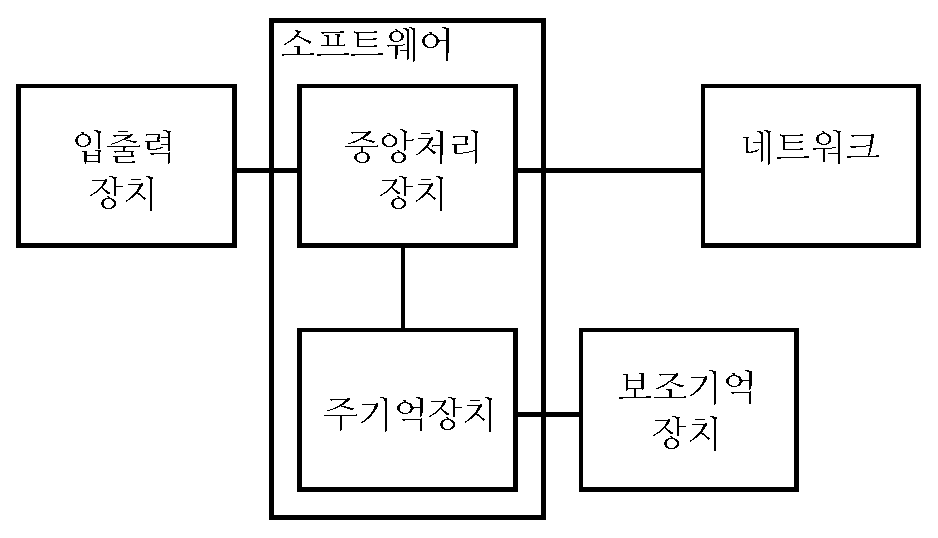
\includegraphics[height=2.50in]{figs2/arch3.eps}}
\afterfig

이번 장에서 {\bf 보조 기억장치(Secondary Memory)} 혹은 파일을 가지고 작업을 시작한다.
보조 기억장치는 전원이 꺼져도 지워지지 않는다.
혹은, USB 플래쉬 드라이브를 사용한 경우에는 프로그램으로부터 작성한 데이터는 시스템에서 제거되어 다른 시스템으로 전송될 수 있다.

우선 텍스트 편집기로 작성한 텍스트 파일을 읽고 쓰는 것에 초점을 맞출 것이다.
나중에 데이터베이스 소프트웨어를 통해서 읽고 쓰도록 설계된 바이너리 파일 데이터베이스를 가지고 어떻게 작업하는지를 살펴볼 것이다.

\section{파일 열기}
\index{파일 (file)!열기 (open)}
\index{열기 함수 (open function)}
\index{함수 (function)!열기 (open)}

하드 디스크 파일을 읽거나 쓸려고 할 때, 파일을 {\bf 열여야(open)} 한다.
파일을 열 때 각 파일 데이터가 어디에 저장되었는지를 알고 있는 운영체제와 커뮤니케이션 한다.
파일을 열 때, 운영체제에 파일이 존재하는지 확인하고 이름으로 파일을 찾도록 요청한다.     
이번 예제에서, 파이썬을 시작한 동일한 폴더에 저장된 {\tt mbox.txt} 파일을 연다.  
\url{www.py4inf.com/code/mbox.txt} 에서 파일을 다운로드할 수 있다.

\beforeverb
\begin{verbatim}
>>> fhand = open('mbox.txt')
>>> print fhand
<open file 'mbox.txt', mode 'r' at 0x1005088b0>
\end{verbatim}
\afterverb
%
\index{파일 핸들 (file handle)}

{\tt open}이 성공하면, 운영체제는 {\bf 파일 핸들(file handle)}을 반환한다.
{\bf 파일 핸들(file handle)}은 파일에 담겨진 실제 데이터는 아니고, 
대신에 데이터를 읽을 수 있도록 사용할 수 있는 ''핸들(handle)''이다.
요청한 파일이 존재하고, 파일을 읽을 수 있는 적절한 권한이 있다면 이제 핸들이 여러분에게 주어졌다.

\beforefig
\centerline{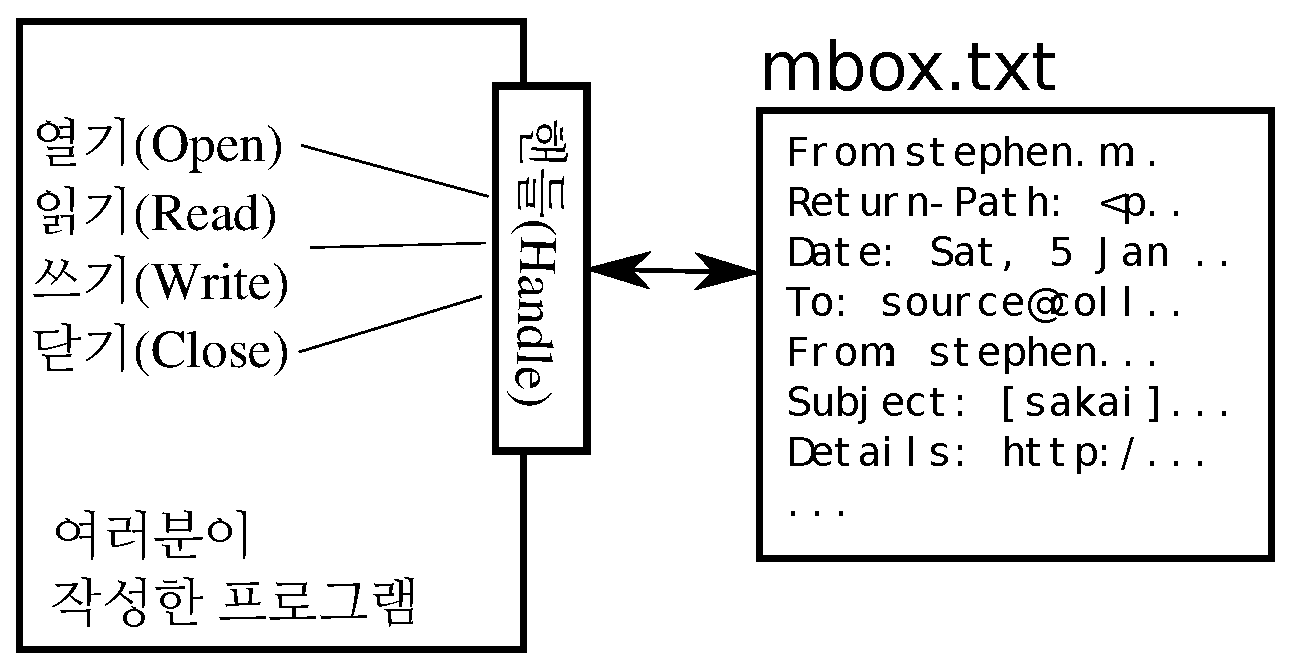
\includegraphics[height=1.75in]{figs2/handle.eps}}
\afterfig

파일이 존재하지 않는다면, {\tt open}은 역추적(traceback) 파일 열기 오류로 실패하고, 파일 콘텐츠에 접근할 핸들도 얻지 못한다.

\beforeverb
\begin{verbatim}
>>> fhand = open('stuff.txt')
Traceback (most recent call last):
  File "<stdin>", line 1, in <module>
IOError: [Errno 2] No such file or directory: 'stuff.txt'
\end{verbatim}
\afterverb
%

나중에 {\tt try}와 {\tt except}를 가지고, 존재하지 않는 파일을 열려고 하는 상황을 좀더 우아하게 처리할 것이다.

\section{텍스트 파일과 라인}

파이썬 문자열이 문자 순서(sequence)로 간주 되듯이 마찬가지로 텍스트 파일은 라인 순서(sequence)로 생각될 수 있다.
예를 들어, 다음은 오픈 소스 프로젝트 개발 팀에서 다양한 참여자들의 전자우편 활동을 기록한 텍스트 파일 샘플이다.

\beforeverb
\begin{alltt}
From stephen.marquard@uct.ac.za Sat Jan  5 09:14:16 2008
Return-Path: <postmaster@collab.sakaiproject.org>
Date: Sat, 5 Jan 2008 09:12:18 -0500
To: source@collab.sakaiproject.org
From: stephen.marquard@uct.ac.za
Subject: [sakai] svn commit: r39772 - content/branches/
Details: http://source.sakaiproject.org/viewsvn/?view=rev\&rev=39772
...
\end{alltt}
\afterverb

상호 의사소통한 전자우편 전체 파일은  \url{www.py4inf.com/code/mbox.txt} 에서 접근 가능하고, 
간략한 버젼 파일은 \url{www.py4inf.com/code/mbox-short.txt}에서 얻을 수 있다.
이들 파일은 다수 전자우편 메시지를 담고 있는 파일로 표준 포맷으로 되어 있다.
"From "으로 시작하는 라인은 메시지 본문과 구별되고, "From: "으로 시작하는 라인은 본문 메시지의 일부다.
더 자세한 정보는 \url{en.wikipedia.org/wiki/Mbox}에서 찾을 수 있다.

파일을 라인으로 쪼개기 위해서, {\bf 새줄(newline)} 문자로 불리는 "줄의 끝(end of the line)"을 표시하는 특수 문자가 있다.

\index{새줄 (newline)}

파이썬에서, 문자열 상수 역슬래쉬-n(\verb"\n")으로 {\bf 새줄(newline)} 문자를 표현한다.
두 문자처럼 보이지만, 사실은 단일 문자다. 인터프리터에 ''stuff''에 입력한 후 변수를 살펴보면, 문자열에 \verb"\n"가 있다.
하지만, {\tt print}문을 사용하여 문자열을 출력하면, 문자열이 새줄 문자에 의해서 두 줄로 쪼개지는 것을 볼 수 있다.

\beforeverb
\begin{verbatim}
>>> stuff = 'Hello\nWorld!'
>>> stuff
'Hello\nWorld!'
>>> print stuff
Hello
World!
>>> stuff = 'X\nY'
>>> print stuff
X
Y
>>> len(stuff)
3
\end{verbatim}
\afterverb
%

문자열 \verb"'X\nY'"의 길이는 \emph{3} 이다. 왜냐하면 새줄(newline) 문자도 한 문자이기 때문이다.

그래서, 파일 라인을 볼 때, 라인 끝을 표시하는 새줄(newline)로 불리는 눈에 보이지 않는 특수 문자가 각 줄의 끝에 있다고 \emph{상상}할 필요가 있다.

% \beforeverb
% \begin{alltt}
% From stephen.marquard@uct.ac.za Sat Jan  5 09:14:16 2008\verb"\n"\\
% Return-Path: <postmaster@collab.sakaiproject.org>\verb"\n"\\
% Date: Sat, 5 Jan 2008 09:12:18 -0500\verb"\n"\\
% To: source@collab.sakaiproject.org\verb"\n"\\
% From: stephen.marquard@uct.ac.za\verb"\n"\\
% Subject: [sakai] svn commit: r39772 - content/branches/\verb"\n"\\
% Details: http://source.sakaiproject.org/viewsvn/?view=rev\&rev=39772\verb"\n"\\
% ...
% \end{alltt}
% \afterverb

그래서, 새줄(newline) 문자는 파일에 있는 문자를 라인으로 분리한다.


\section{파일 읽어오기}

\index{파일 (file)!읽어 오기 (reading)}
\index{계수기 (counter)}

{\bf 파일 핸들(file handle)}이 파일 자료를 담고 있지 않지만, 
{\tt for} 루프를 사용하여 파일 각 라인을 읽고 라인수를 세는 것을 쉽게 구축할 수 있다.

\beforeverb
\begin{verbatim}
fhand = open('mbox.txt')
count = 0
for line in fhand:
    count = count + 1
print 'Line Count:', count

python open.py 
Line Count: 132045
\end{verbatim}
\afterverb
%

파일 핸들을 {\tt for} 루프 순서(sequence)로 사용할 수 있다. 
{\tt for} 루프는 단순히 파일 라인 수를 세고 전체 라인수를 출력한다.
{\tt for} 루프를 대략 일반어로 풀어 말하면, "파일 핸들로 표현되는 파일 각 라인마다, {\tt count} 변수에 1 씩 더한다"

{\tt open} 함수가 전체 파일을 바로 읽지 못하는 이유는 파일이 수 기가 바이트 파일 크기를 가질 수도 있기 때문이다.
{\tt open} 문장은 파일 크기에 관계없이 파일을 여는데 시간이 동일하게 걸린다. 
실질적으로 {\tt for} 루프가 파일로부터 자료를 읽어오는 역할을 한다.

{\tt for} 루프를 사용해서 이 같은 방식으로 파일을 읽어올 때, 새줄(newline) 문자를 사용해서 파일 자료를 라인 단위로 쪼갠다.
파이썬에서 새줄(newline) 문자까지 각 라인 단위로 읽고, 
{\tt for} 루프가 매번 반복할 때마다 {\tt line} 변수에 새줄(newline)을 마지막 문자로 포함한다.

{\tt for} 루프가 데이터를 한번에 한줄씩 읽어오기 때문에, 데이터를 저장할 주기억장치 저장공간을 소진하지 않고, 매우 큰 파일을 효과적으로 읽어서 라인을 셀 수 있다.
각 라인별로 읽고, 세고, 그리고 나서 폐기되기 때문에, 매우 적은 저장공간을 사용해서 어떤 크기의 파일도 상기 프로그램을 사용하여 라인을 셀 수 있다.

만약 주기억장치 크기에 비해서 상대적으로 작은 크기의 파일이라는 것을 안다면, 
전체 파일을 파일 핸들로 {\tt read} 메쏘드를 사용해서 하나의 문자열로 읽어올 수 있다.

\beforeverb
\begin{verbatim}
>>> fhand = open('mbox-short.txt')
>>> inp = fhand.read()
>>> print len(inp)
94626
>>> print inp[:20]
From stephen.marquar
\end{verbatim}
\afterverb
%

상기 예제에서, {\tt mbox-short.txt} 전체 파일 콘텐츠(94,626 문자)를 변수 {\tt inp}로 바로 읽었다.
문자열 슬라이싱을 사용해서 {\tt inp}에 저장된 문자열 자료 첫 20 문자를 출력한다.

파일이 이런 방식으로 읽혀질 때, 모든 라인과 새줄(newline)문자를 포함한 모든 문자는 변수 {\tt inp}에 대입된 매우 큰 문자열이다.
파일 데이터가 컴퓨터 주기억장치가 안정적으로 감당해 낼 수 있을때만, 
이런 형식의 {\tt open} 함수가 사용될 수 있다는 것을 기억하라.

만약 주기억장치가 감당해 낼 수 없는 매우 파일 크기가 크다면, {\tt for}나 {\tt while} 루프를 사용해서 파일을 쪼개서 읽는 프로그램을 작성해야 한다.

\section{파일 검색}

파일 데이터를 검색할 때, 흔한 패턴은 파일을 읽고, 대부분 라인은 건너뛰고, 특정 기준을 만족하는 라인만 처리하는 것이다.
간단한 검색 메카니즘을 구현하기 위해서 파일을 읽는 패턴과 문자열 {\bf 메쏘드}를 조합한다.

\index{필터 패턴 (filter pattern)}
\index{패턴 (pattern)!필터 (filter)}

예를 들어, 파일을 읽고, ``From:''으로 시작하는 라인만 출력하고자 한다면, 
{\bf startswith} 문자열 메쏘드를 사용해서 원하는 접두사로 시작하는 라인만을 선택한다.

\beforeverb
\begin{verbatim}
fhand = open('mbox-short.txt')
for line in fhand:
    if line.startswith('From:') :
        print line
\end{verbatim}
\afterverb
%

이 프로그램이 실행하면 다음 출력값을 얻는다.

\beforeverb
\begin{verbatim}
From: stephen.marquard@uct.ac.za

From: louis@media.berkeley.edu

From: zqian@umich.edu

From: rjlowe@iupui.edu
...
\end{verbatim}
\afterverb
%

''From:''으로만 시작하는 라인만 출력하기 때문에 출력값은 훌륭해 보인다.
하지만, 왜 여분으로 빈 라인이 보이는 걸까?
원인은 눈에 보이지 않는 {\bf 새줄(newline)} 문자 때문이다.
각 라인이 새줄(newline)로 끝나서 변수 {\bf line}에 새줄(newline)이 포함되고 
{\tt print}문이 추가로 새줄(newline)을 추가해서 결국 우리가 보기에는 두 줄 효과가 나타난다.

마지막 문자를 제외하고 모든 것을 출력하기 위해서 라인 슬라이싱(slicing)을 할수 있지만, 
좀더 간단한 접근법은 다음과 같이 문자열 오른쪽 끝에서부터 공백을 벗겨내는 {\bf rstrip} 메쏘드를 사용하는 것인다.

\beforeverb
\begin{verbatim}
fhand = open('mbox-short.txt')
for line in fhand:
    line = line.rstrip()
    if line.startswith('From:') :
        print line
\end{verbatim}
\afterverb
%

프로그램을 실행하면, 다음 출력값을 얻는다.

\beforeverb
\begin{verbatim}
From: stephen.marquard@uct.ac.za
From: louis@media.berkeley.edu
From: zqian@umich.edu
From: rjlowe@iupui.edu
From: zqian@umich.edu
From: rjlowe@iupui.edu
From: cwen@iupui.edu
...
\end{verbatim}
\afterverb
%

파일 처리 프로그램이 점점 더 복잡해짐에 따라 {\tt continue}를 사용해서 검색 루프(search loop)를 구조화할 필요가 있다.
검색 루프의 기본 아이디어는 ''흥미로운'' 라인을 집중적으로 찾고, ''흥미롭지 않은'' 라인은 효과적으로 건너뛰는 것이다.
그리고 나서 흥미로운 라인을 찾게되면, 그 라인에서 특정 연산을 수행하는 것이다.

다음과 같이 루프를 구성해서 흥미롭지 않은 라인은 건떠뛰는 패턴을 따르게 한다.

\beforeverb
\begin{verbatim}
fhand = open('mbox-short.txt')
for line in fhand:
    line = line.rstrip()
    # Skip 'uninteresting lines'
    if not line.startswith('From:') :
        continue
    # Process our 'interesting' line
    print line
\end{verbatim}
\afterverb
%

프로그램의 출력값은 동일하다. 
흥미롭지 않는 라인은 ''From:''으로 시작하지 않는 라인이라 {\tt continue}문을 사용해서 건너뛴다.
''흥미로운'' 라인 (즉, ''From:''으로 시작하는 라인)에 대해서는 연산처리를 수행한다. 

{\tt find} 문자열 메쏘드를 사용해서 검색 문자열이 라인 어디에 있는지를 찾아주는 텍스트 편집기 검색기능을 모사(simulation)할 수 있다.
{\tt find} 메쏘드는 다른 문자열 내부에 검색하는 문자열이 있는지 찾고, 문자열 위치를 반환하거나, 만약 문자열이 없다면 -1을 반환하기 때문에,
``@uct.ac.za''(남아프리카 케이프 타운 대학으로부터 왔다) 문자열을 포함하는 라인을 검색하기 위해 다음과 같이 루프를 작성한다.

\beforeverb
\begin{verbatim}
fhand = open('mbox-short.txt')
for line in fhand:
    line = line.rstrip()
    if line.find('@uct.ac.za') == -1 : 
        continue
    print line
\end{verbatim}
\afterverb
%
출력결과는 다음과 같다.

\beforeverb
\begin{verbatim}
From stephen.marquard@uct.ac.za Sat Jan  5 09:14:16 2008
X-Authentication-Warning: set sender to stephen.marquard@uct.ac.za using -f
From: stephen.marquard@uct.ac.za
Author: stephen.marquard@uct.ac.za
From david.horwitz@uct.ac.za Fri Jan  4 07:02:32 2008
X-Authentication-Warning: set sender to david.horwitz@uct.ac.za using -f
From: david.horwitz@uct.ac.za
Author: david.horwitz@uct.ac.za
...
\end{verbatim}
\afterverb
%

\section{사용자가 파일명을 선택하게 만들기}

매번 다른 파일을 처리할 때마다 파이썬 코드를 편집하고 싶지는 않다. 
매번 프로그램이 실행될 때마다, 파일명을 사용자가 입력하도록 만드는 것이 좀더 유용할 것이다. 
그래서 파이썬 코드를 바꾸지 않고, 다른 파일에 대해서도 동일한 프로그램을 사용하도록 만들자.

다음과 같이 \verb"raw_input"을 사용해서 사용자로부터 파일명을 읽어 프로그램을 실행하는 것이 단순하다.

\beforeverb
\begin{verbatim}
fname = raw_input('Enter the file name: ')
fhand = open(fname)
count = 0
for line in fhand:
    if line.startswith('Subject:') :
        count = count + 1
print 'There were', count, 'subject lines in', fname
\end{verbatim}
\afterverb
%

사용자로부터 파일명을 읽고 변수 {\tt fname}에 저장하고, 그 파일을 연다. 
이제 다른 파일에 대해서도 반복적으로 프로그램을 실행할 수 있다.

\beforeverb
\begin{verbatim}
python search6.py 
Enter the file name: mbox.txt
There were 1797 subject lines in mbox.txt

python search6.py 
Enter the file name: mbox-short.txt
There were 27 subject lines in mbox-short.txt
\end{verbatim}
\afterverb
%

다음 절을 엿보기 전에, 상기 프로그램을 살펴보고 자신에게 다음을 질문해 보자.
"여기서 어디가 잘못될 수 있는가?" 혹은 
"이 작고 멋진 프로그램에 트레이스백(traceback)을 남기고 바로 끝나게 하여,
결국 사용자 눈에는 좋지 않은 프로그램이라는 인상을 남길 수 있도록 우리의 친절한 사용자는 무엇을 할 수 있을까?

\section{{\tt try, except, open} 사용하기}

제가 여러분에게 엿보지 말라고 말씀드렸습니다. 이번이 마지막 기회입니다.
사용자가 파일명이 아닌 뭔가 다른 것을 입력하면 어떻게 될까요?

\beforeverb
\begin{verbatim}
python search6.py 
Enter the file name: missing.txt
Traceback (most recent call last):
  File "search6.py", line 2, in <module>
    fhand = open(fname)
IOError: [Errno 2] No such file or directory: 'missing.txt'

python search6.py 
Enter the file name: na na boo boo
Traceback (most recent call last):
  File "search6.py", line 2, in <module>
    fhand = open(fname)
IOError: [Errno 2] No such file or directory: 'na na boo boo'
\end{verbatim}
\afterverb
%

웃지마시구요, 사용자는 결국 여러분이 작성한 프로그램을 망가뜨리기 위해 고의든 악의를 가지든 가능한 모든 수단을 강구할 것입니다.
사실, 소프트웨어 개발팀의 중요한 부분은 {\bf 품질 보증(Quality Assurance, QA)}이라는 조직이다. 
품질보증 조직은 프로그래머가 만든 소프트웨어를 망가뜨리기 위해 가능한 말도 안 되는 것을 합니다.

\index{품질 보증 (Quality Assurance)}
\index{QA}

사용자가 소프트웨어를 제품으로 구매하거나, 주문형으로 개발하는 프로그램에 대해 월급을 지급하던지 관계없이 
품질보증 조직은 프로그램이 사용자에게 전달되기 전까지 프로그램 오류를 발견할 책임이 있다.
그래서 품질보증 조직은 프로그래머의 최고의 친구다.

\index{try 문장 (try statement)}
\index{문장 (statement)!try}
\index{open 함수 (open function)}
\index{함수 (function)!open}
\index{예외 (exception)!입출력 오류 (IOError)}
\index{입출력 오류 (IOError)}

프로그램 오류를 찾았기 때문에, {\tt try}/{\tt except} 구조를 사용해서 오류를 우아하게 고쳐봅시다.
{\tt open} 호출이 잘못될 수 있다고 가정하고, {\tt open} 호출이 실패할 때를 대비해서 다음과 같이 복구 코드를 추가한다.

\beforeverb
\begin{verbatim}
fname = raw_input('Enter the file name: ')
try:
    fhand = open(fname)
except:
    print 'File cannot be opened:', fname
    exit()

count = 0
for line in fhand:
    if line.startswith('Subject:') : 
        count = count + 1
print 'There were', count, 'subject lines in', fname
\end{verbatim}
\afterverb
%

{\tt exit}함수가 프로그램을 끝낸다. 
결코 돌아오지 않는 함수를 호출한 것이다.
이제 사용자 혹은 품질 보증 조직에서 올바르지 않거나 어처구니 없는 파일명을 입력했을 때, 
``catch''로 잡아서 우아하게 복구한다.

\beforeverb
\begin{verbatim}
python search7.py
Enter the file name: mbox.txt
There were 1797 subject lines in mbox.txt

python search7.py
Enter the file name: na na boo boo
File cannot be opened: na na boo boo
\end{verbatim}
\afterverb
%
\index{파이썬스러운 (Pythonic)}

파이썬 프로그램을 작성할 때 {\tt open} 호출을 보호하는 것은 {\tt try}, {\tt except}의 적절한 사용 예제가 된다.
''파이썬 방식(Python way)''으로 무언가를 작성할 때, ''파이썬스러운(Pythonic)''이라는 용어를 사용한다.
상기 파일을 여는 예제는 파이썬스러운 방식의 좋은 예가 된다고 말한다.

파이썬에 좀더 자신감이 생기게 되면, 다른 파이썬 프로그래머와 동일한 문제에 대해 
두 가지 동치하는 해답을 가지고 어떤 접근법이 좀더 "파이썬스러운지"에 대한 현답을 찾는데도 관여하게 된다.

"좀더 파이썬스럽게" 되는 이유는 프로그래밍이 엔지니어링적인 면과 예술적인 면을 동시에 가지고 있기 때문이다.
항상 무언가를 단지 작동하는 것에만 관심이 있지 않고, 프로그램으로 작성한 해결책이 좀더 우아하고, 다른 동료에 의해서 우아한 것으로 인정되기를 또한 원합니다.

\section{파일에 쓰기}

\index{파일 (file)!쓰기 (writing)}

파일에 쓰기 위해서는 두 번째 매개 변수로 \verb"'w'" 모드로 파일을 열어야 한다.

\beforeverb
\begin{verbatim}
>>> fout = open('output.txt', 'w')
>>> print fout
<open file 'output.txt', mode 'w' at 0xb7eb2410>
\end{verbatim}
\afterverb
%

파일이 이미 존재하는데 쓰기 모드에서 파일을 여는 것은 이전 데이터를 모두 지워버리고, 
깨끗한 파일 상태에서 다시 시작되니 주의가 필요하다. 
만약 파일이 존재하지 않는다면, 새로운 파일이 생성된다.

파일 핸들 객체의 {\tt write} 메쏘드는 데이터를 파일에 저장한다.

\beforeverb
\begin{verbatim}
>>> line1 = 'This here's the wattle,\n'
>>> fout.write(line1)
\end{verbatim}
\afterverb
%
\index{새줄 (newline)}

다시 한번, 파일 객체는 마지막 포인터가 어디에 있는지 위치를 추적해서, 
만약 {\tt write} 메쏘드를 다시 호출하게 되면, 새로운 데이터를 파일 끝에 추가한다.

라인을 끝내고 싶을 때, 명시적으로 새줄(newline) 문자를 삽입해서 파일에 쓰도록 라인 끝을 필히 관리해야 한다.

{\tt print}문은 자동적으로 새줄(newline)을 추가하지만, {\tt write} 메쏘드는 자동적으로 새줄(newline)을 추가하지는 않는다.

\beforeverb
\begin{verbatim}
>>> line2 = 'the emblem of our land.\n'
>>> fout.write(line2)
\end{verbatim}
\afterverb
%

파일 쓰기가 끝났을 때, 파일을 필히 닫아야 한다.
파일을 닫는 것은 데이터 마지막 비트까지 디스크에 물리적으로 쓰여져서, 
전원이 나가더라도 자료가 유실되지 않는 역할을 한다.

\beforeverb
\begin{verbatim}
>>> fout.close()
\end{verbatim}
\afterverb
%

파일 읽기로 연 파일을 닫을 수 있지만, 몇개 파일을 열어 놓았다면 약간 단정치 못하게 끝날 수 있습니다. 
왜냐하면 프로그램이 종료될 때 열린 모든 파일이 닫혀졌는지 파이썬이 확인하기 때문이다. 
파일에 쓰기를 할 때는, 파일을 명시적으로 닫아서 예기치 못한 일이 발생할 여지를 없애야 한다.

\index{close 메쏘드 (close method)}
\index{메쏘드 (method)!close}

\section{디버깅}

\index{디버깅 (debugging)}
\index{공백 (whitespace)}

파일을 읽고 쓸 때, 공백 때문에 종종 문제에 봉착한다.
이런 종류의 오류는 공백, 탭, 새줄(newline)이 눈에 보이지 않기 때문에 디버그하기도 쉽지 않다.

\beforeverb
\begin{verbatim}
>>> s = '1 2\t 3\n 4'
>>> print s
1 2	 3
 4
\end{verbatim}
\afterverb

\index{repr 함수 (repr function)}
\index{함수 (function)!repr}
\index{문자열 표현 (string representation)}

내장함수 {\tt repr}이 도움이 될 수 있다. 
인자로 임의 객체를 잡아 객체 문자열 표현으로 반환한다.
문자열 공백문자는 역슬래쉬 순서(sequence)로 나타냅니다.

\beforeverb
\begin{verbatim}
>>> print repr(s)
'1 2\t 3\n 4'
\end{verbatim}
\afterverb

디버깅에 도움이 될 수 있다.

여러분이 봉착하는 또 다른 문제는 다른 시스템에서는 라인 끝을 표기하기 위해서 다른 문자를 사용한다는 점이다.
어떤 시스템은 \verb"\n" 으로 새줄(newline)을 표기하고, 다른 시스템은 \verb"\r"으로 반환 문자(return character)를 사용한다.
둘다 모두 사용하는 시스템도 있다. 
파일을 다른 시스템으로 이식한다면, 이러한 불일치가 문제를 야기한다.

\index{라인 끝 문자 (end of line character)}

대부분의 시스템에는 A 포맷에서 B 포멧으로 변환하는 응용프로그램이 있다.
\url{wikipedia.org/wiki/Newline} 에서 응용프로그램을 찾을 수 있고, 좀더 많은 것을 읽을 수 있다.
물론, 여러분이 직접 프로그램을 작성할 수도 있다.

% TBD - Doesn't Python take care of this for us????

\section{용어정의}

\begin{description}

\item[잡기(catch):] {\tt try}와 {\tt except} 문을 사용해서 프로그램이 끝나는 예외 상황을 방지하는 것.
\index{잡기 (catch)}

\item[새줄(newline):] 라인의 끝을 표기 위한 파일이나 문자열에 사용되는 특수 문자.
\index{새줄 (newline)}

\item[파이썬스러운(Pythonic):] 파이썬에서 우아하게 작동하는 기술. ''try와 catch를 사용하는 것은 파일이 없는 경우를 복구하는 파이썬스러운 방식이다.''
\index{파이썬스러운 (Pythonic)}

\item[품질 보증(Quality Assurance, QA):] 소프트웨어 제품의 전반적인 품질을 보중하는데 집중하는 사람이나 조직.
품질 보증은 소프트웨어 제품을 시험하고, 제품이 시장에 출시되기 전에 문제를 확인하는데 관여한다.
\index{품질 보증 (Quality Assurance)}
\index{QA}

\item[텍스트 파일(text file):] 하드디스크 같은 영구 저장소에 저장된 일련의 문자 집합.
\index{텍스트 파일 (text file)}

\end{description}

\section{연습문제}

\begin{ex}
파일을 읽고 한줄씩 파일의 내용을 모두 대문자로 출력하는 프로그램을 작성하세요.
프로그램을 싱행하면 다음과 같이 보일 것입니다.

\beforeverb
\begin{verbatim}
python shout.py
Enter a file name: mbox-short.txt
FROM STEPHEN.MARQUARD@UCT.AC.ZA SAT JAN  5 09:14:16 2008
RETURN-PATH: <POSTMASTER@COLLAB.SAKAIPROJECT.ORG>
RECEIVED: FROM MURDER (MAIL.UMICH.EDU [141.211.14.90])
	 BY FRANKENSTEIN.MAIL.UMICH.EDU (CYRUS V2.3.8) WITH LMTPA;
	 SAT, 05 JAN 2008 09:14:16 -0500
\end{verbatim}
\afterverb
%
\url{www.py4inf.com/code/mbox-short.txt}에서 파일을 다운로드 받으세요.
\end{ex}

\begin{ex}

파일명을 입력받아, 파일을 읽고, 다음 형식의 라인을 찾는 프로그램을 작성하세요.

\beforeverb
\begin{alltt}
X-DSPAM-Confidence: {\bf 0.8475}
\end{alltt}
\afterverb

``X-DSPAM-Confidence:''로 시작하는 라인을 만나게 되면, 부동 소수점 숫자를 뽑아내기 위해 해당 라인을 별도로 보관하세요.
라인 수를 세고, 라인으로부터 스팸 신뢰값의 총계를 계산하세요. 
파일의 끝에 도달할 했을 때, 평균 스팸 신뢰도를 출력하세요.

\beforeverb
\begin{verbatim}
Enter the file name: mbox.txt
Average spam confidence: 0.894128046745

Enter the file name: mbox-short.txt
Average spam confidence: 0.750718518519
\end{verbatim}
\afterverb
%
{\tt mbox.txt}와 {\tt mbox-short.txt} 파일에 작성한 프로그램을 시험하세요.
\end{ex}

\begin{ex}

때때로, 프로그래머가 지루해지거나, 약간 재미를 목적으로, 프로그램에 무해한 {\bf 부활절 달걀}(Easter Egg, \url{en.wikipedia.org/wiki/Easter_egg_(media)})을 넣습니다.
사용자가 파일명을 입력하는 프로그램을 변형시켜, 'na na boo boo'로 파일명을 정확하게 입력했을 때, 재미있는 메시지를 출력하는 프로그램을 작성하세요.
파일이 존재하거나, 존재하지 않는 다른 모든 파일에 대해서도 정상적으로 작동해야 합니다. 
여기 프로그램을 실행한 견본이 있습니다.

\beforeverb
\begin{verbatim}
python egg.py 
Enter the file name: mbox.txt
There were 1797 subject lines in mbox.txt

python egg.py 
Enter the file name: missing.tyxt
File cannot be opened: missing.tyxt

python egg.py 
Enter the file name: na na boo boo
NA NA BOO BOO TO YOU - You have been punk'd!
\end{verbatim}
\afterverb
%

프로그램에 부활절 달걀을 넣도록 격려하지는 않습니다. 단지 연습입니다.

\end{ex}


% LaTeX source for ``Python for Informatics: Exploring Information''
% Copyright (c)  2010-  Charles R. Severance, All Rights Reserved

\chapter{리스트 (List)}

\index{리스트 (list)}
\index{자료형 (type)!리스트 (list)}

\section{리스트는 순서(sequence)다.}

문자열처럼, {\bf 리스트(list)}는 값의 순서(sequence)다. 
문자열에서, 값은 문자지만, 리스트에서는 임의 자료형(type)도 될 수 있다.
리스트 값은 {\bf 요소(elements)}나 때때로 {\bf 항목(items)}으로 불린다.

\index{요소 (element)}
\index{순서 (sequence)}
\index{항목 (item)}

신규 리스틀 생성하는 방법은 여러 가지가 있다. 
가장 간단한 방법은 꺾쇠 괄호(\verb"[" 와 \verb"]")로 요소를 감싸는 것이다.

\beforeverb
\begin{verbatim}
[10, 20, 30, 40]
['crunchy frog', 'ram bladder', 'lark vomit']
\end{verbatim}
\afterverb
%

첫번째 예제는 4개 정수 리스트다. 
두번째 예제는 3개 문자열 리스트다.
문자열 요소가 동일한 자료형(type)일 필요는 없다. 
다음 리스트는 문자열, 부동 소수점 숫자, 정수, (아!) 또 다른 리스트를 담고 있다.

\beforeverb
\begin{verbatim}
['spam', 2.0, 5, [10, 20]]
\end{verbatim}
\afterverb
%

또 다른 리스트 내부에 리스트가 {\bf 중첩(nested)}되어 있다.

\index{중첩 리스트 (nested list)}
\index{리스트 (list)!중첩 (nested)}

어떤 요소도 담고 있지 않는 리스트를 빈 리스트(empty list)라고 부르고, 빈 꺾쇠 괄호(''[]'')로 생성한다.

\index{빈 리스트 (empty list)}
\index{리스트 (list)!빈 (empty)}

예상했듯이, 리스트 값을 변수에 대입할 수 있다.

\beforeverb
\begin{verbatim}
>>> cheeses = ['Cheddar', 'Edam', 'Gouda']
>>> numbers = [17, 123]
>>> empty = []
>>> print cheeses, numbers, empty
['Cheddar', 'Edam', 'Gouda'] [17, 123] []
\end{verbatim}
\afterverb
%

\index{assignment}

\section{리스트는 변경가능하다.}

\index{리스트 (list)!요소 (element)}
\index{접근 (access)}
\index{인덱스 (index)}
\index{꺾쇠 연산자 (bracket operator)}
\index{연산자 (operator)!꺾쇠 (bracket)}

리스트 요소에 접근하는 구문은 문자열 문자에 접근하는 것과 동일한 꺾쇠 괄호 연산자다.
꺽쇠 괄호 내부 표현식은 인덱스를 명세한다. 기억할 것은 인덱스는 0 에서부터 시작한다는 것이다.

\beforeverb
\begin{verbatim}
>>> print cheeses[0]
Cheddar
\end{verbatim}
\afterverb
%

문자열과 달리, 리스트 항목 순서를 바꾸거나, 리스트에 새로운 항목을 다시 대입할 수 있기 때문에 리스트는 변경가능하다.
꺾쇠 괄호 연산자가 대입문 왼쪽편에 나타날 때, 새로 대입될 리스트 요소를 나타낸다.

\index{변경성 (mutability)}

\beforeverb
\begin{verbatim}
>>> numbers = [17, 123]
>>> numbers[1] = 5
>>> print numbers
[17, 5]
\end{verbatim}
\afterverb
%

리스트 {\tt numbers} 첫번째 요소는 123 값을 가지고 있었으나, 이제 5 값을 가진다.

\index{인덱스 (index)!0 에서 시작 (starting at zero)}
\index{0 (zero), 인덱스 시작점 (index starting at)}

리스트를 인덱스와 요소의 관계로 생각할 수 있다. 
이 관계를 {\bf 매핑(mapping)}이라고 부른다. 
각각의 인덱스는 요소 중 하나에 대응(''maps to'')된다.

\index{항목 대입 (item assignment)}
\index{대입 (assignment)!항목 (item)}

리스트 인덱스는 문자열 인덱스와 동일한 방식으로 동작한다.

\begin{itemize}

\item 어떠한 정수 표현식도 인덱스로 사용할 수 있다.

\item 존재하지 않는 요소를 읽거나 쓰려고 하면, {\tt 인덱스 오류 (IndexError)}가 발생한다.

\index{예외 (exception)!인덱스 오류 (IndexError)}
\index{인덱스 오류 (IndexError)}

\item 인덱스가 음의 값이면, 리스트 끝에서부터 역으로 센다.

\end{itemize}

\index{리스트 (list)!인덱스 (index)}

\index{리스트 (list)!소속 (membership)}
\index{소속 (membership)!리스트 (list)}
\index{in 연산자 (in operator)}
\index{연산자 (operator)!in}

{\tt in} 연산자도 또한 리스트에서 동작하니 사용할 수 있다.

\beforeverb
\begin{verbatim}
>>> cheeses = ['Cheddar', 'Edam', 'Gouda']
>>> 'Edam' in cheeses
True
>>> 'Brie' in cheeses
False
\end{verbatim}
\afterverb

\section{리스트 운행법}
\index{리스트 (list)!운행법 (traversal)}
\index{운행법 (traversal)!리스트 (list)}
\index{for 루프 (for loop)}
\index{루프 (loop)!for}
\index{문장 (statement)!for}

리스트 요소를 운행하는 가장 흔한 방법은 {\tt for}문을 사용하는 것이다.
문자열에서 사용한 것과 구문은 동일하다.

\beforeverb
\begin{verbatim}
for cheese in cheeses:
    print cheese
\end{verbatim}
\afterverb
%

리스트 요소를 읽기만 한다면 이것만으로도 잘 동작한다. 
하지만, 리스트 요소를 쓰거나, 갱신하는 경우, 인텍스가 필요하다. 
리스트 요소를 쓰거나 갱신하는 일반적인 방법은 {\tt range}와 {\tt len} 함수를 조합하는 것이다.

\index{루핑 (looping)!인덱스를 가지고 (with indices)}
\index{인덱스 (index)!루핑 (looping with)}

\beforeverb
\begin{verbatim}
for i in range(len(numbers)):
    numbers[i] = numbers[i] * 2
\end{verbatim}
\afterverb
%

상기 루프는 리스트를 운행하고 각 요소를 갱신한다. 
{\tt len} 함수는 리스트 요소 갯수를 반환한다.
{\tt range} 함수는 0 에서 $n-1$ 까지 리스트 인텍스를 반환한다. 
여기서, $n$은 리스트 길이다.
매번 루프가 반복될 때마다, {\tt i}는 다음 요소 인덱스를 얻는다. 
몸통 부문 대입문은 {\tt i}를 사용해서 요소의 이전 값을 읽고 새 값을 대입한다.

\index{항목 갱신 (item update)}
\index{갱신 (update)!항목 (item)}

빈 리스트에 대해서 {\tt for}문은 결코 몸통 부문을 실행하지 않는다.

\beforeverb
\begin{verbatim}
for x in empty:
    print 'This never happens.'
\end{verbatim}
\afterverb
%

리스트가 또 다른 리스트를 담을 수 있지만, 중첩된 리스트는 여전히 요소 하나로 간주된다. 
다음 리스트 길이는 4 이다.

\index{중첩 리스트 (nested list)}
\index{리스트 (list)!중첩 (nested)}

\beforeverb
\begin{verbatim}
['spam', 1, ['Brie', 'Roquefort', 'Pol le Veq'], [1, 2, 3]]
\end{verbatim}
\afterverb

\section{리스트 연산자}
\index{리스트 (list)!연산 (operation)}

{\tt +} 연산자는 리스트를 결합한다.

\index{연결 (concatenation)!리스트 (list)}
\index{리스트 (list)!연결 (concatenation)}

\beforeverb
\begin{verbatim}
>>> a = [1, 2, 3]
>>> b = [4, 5, 6]
>>> c = a + b
>>> print c
[1, 2, 3, 4, 5, 6]
\end{verbatim}
\afterverb
%

유사하게 {\tt *} 연산자는 주어진 횟수만큼 리스트를 반복한다.

\index{반복 (repetition)!리스트 (list)}
\index{리스트 (list)!반복 (repetition)}

\beforeverb
\begin{verbatim}
>>> [0] * 4
[0, 0, 0, 0]
>>> [1, 2, 3] * 3
[1, 2, 3, 1, 2, 3, 1, 2, 3]
\end{verbatim}
\afterverb
%

첫 예제는 {\tt [0]}을 4회 반복한다. 
두 번째 예제는 {\tt [1, 2, 3]} 리스트를 3회 반복한다.

\section{리스트 슬라이스(List slices)}

\index{슬라이스 연산자 (slice operator)}
\index{연산자 (operator)!슬라이스 (slice)}
\index{인덱스 (index)!슬라이스 (slice)}
\index{리스트 (list)!슬라이스 (slice)}
\index{슬라이스 (slice)!리스트 (list)}

슬라이스 연산자는 리스트에도 또한 동작한다.

\beforeverb
\begin{verbatim}
>>> t = ['a', 'b', 'c', 'd', 'e', 'f']
>>> t[1:3]
['b', 'c']
>>> t[:4]
['a', 'b', 'c', 'd']
>>> t[3:]
['d', 'e', 'f']
\end{verbatim}
\afterverb
%

첫 번째 인덱스를 생략하면, 슬라이스는 처음부터 시작한다. 
두 번째 인덱스를 생략하면, 슬라이스는 끝까지 간다.
그래서 양쪽의 인덱스를 생략하면, 슬라이스 결과는 전체 리스트를 복사한 것이 된다.

\index{리스트 (list)!복사 (copy)}
\index{슬라이스 (slice)!복사 (copy)}
\index{복사 (copy)!슬라이스 (slice)}

\beforeverb
\begin{verbatim}
>>> t[:]
['a', 'b', 'c', 'd', 'e', 'f']
\end{verbatim}
\afterverb
%

리스트는 변경이 가능하기 때문에 리스트를 접고, 돌리고, 훼손하는 연산을 수행하기 전에 복사본을 만들어 두는 것이 유용하다.

\index{변경성 (mutability)}

대입문 왼편의 슬라이스 연산자로 복수의 요소를 갱신할 수 있다.

\index{슬라이스 (slice)!갱신 (update)}
\index{갱신 (update)!슬라이스 (slice)}

\beforeverb
\begin{verbatim}
>>> t = ['a', 'b', 'c', 'd', 'e', 'f']
>>> t[1:3] = ['x', 'y']
>>> print t
['a', 'x', 'y', 'd', 'e', 'f']
\end{verbatim}
\afterverb
%

\section{리스트 메쏘드}

\index{리스트 (list)!메쏘드 (method)}
\index{메쏘드 (method), 리스트 (list)}

파이썬은 리스트에 연산하는 메쏘드를 제공한다. 
예를 들어, {\tt 덧붙이기 (append)} 메쏘드는 리스트 끝에 신규 요소를 추가한다.

\index{덧붙이기 메쏘드 (append method)}
\index{메쏘드 (method)!덧붙이기 (append)}

\beforeverb
\begin{verbatim}
>>> t = ['a', 'b', 'c']
>>> t.append('d')
>>> print t
['a', 'b', 'c', 'd']
\end{verbatim}
\afterverb
%
{\tt 확장 (extend)} 메쏘드는 인자로 리스트를 받아 모든 요소를 리스트에 덧붙인다.

\index{확장 메쏘드 (extend method)}
\index{메쏘드 (method)!확장 (extend)}

\beforeverb
\begin{verbatim}
>>> t1 = ['a', 'b', 'c']
>>> t2 = ['d', 'e']
>>> t1.extend(t2)
>>> print t1
['a', 'b', 'c', 'd', 'e']
\end{verbatim}
\afterverb
%

상기 예제는 {\tt t2} 리스트를 변경없이 그냥 둔다.

{\tt 정렬 (sort)} 메쏘드는 낮음에서 높음으로 리스트 요소를 정렬한다.

\index{정렬 메쏘드 (sort method)}
\index{메쏘드 (method)!정렬 (sort)}

\beforeverb
\begin{verbatim}
>>> t = ['d', 'c', 'e', 'b', 'a']
>>> t.sort()
>>> print t
['a', 'b', 'c', 'd', 'e']
\end{verbatim}
\afterverb
%

대부분의 리스트 메쏘드는 보이드(void)여서, 리스트를 변경하고 {\tt None}을 반환한다.
우연히 {\tt t = t.sort()} 이렇게 작성한다면, 결과에 실망할 것이다.

\index{void 메쏘드 (void method)}
\index{메쏘드 (method)!void}
\index{None 특수값 (None special value)}
\index{특수값 (special value)!None}

\section{요소 삭제}

\index{요소 삭제 (element deletion)}
\index{삭제 (deletion), 리스트 요소 (element of list)}

리스트 요소를 삭제하는 방법이 몇 가지 있다. 
리스트 요소 인덱스를 알고 있다면, {\tt 팝 (pop)} 메쏘드를 사용한다.

\index{팝 메쏘드 (pop method)}
\index{메쏘드 (method)!팝 (pop)}

\beforeverb
\begin{verbatim}
>>> t = ['a', 'b', 'c']
>>> x = t.pop(1)
>>> print t
['a', 'c']
>>> print x
b
\end{verbatim}
\afterverb
%

{\tt 팝(pop)} 메쏘드는 리스트를 변경하여  제거된 요소를 반환한다.
인덱스를 주지 않으면, 마지막 요소를 지우고 반환한다.

요소에서 제거된 값이 필요없다면, {\tt del} 연산자를 사용한다.

\index{del 연산자 (del operator)}
\index{연산자 (operator)!del}

\beforeverb
\begin{verbatim}
>>> t = ['a', 'b', 'c']
>>> del t[1]
>>> print t
['a', 'c']
\end{verbatim}
\afterverb
%

(인덱스가 아닌) 제거할 요소값을 알고 있다면, {\tt 제거 (remove)} 메쏘드를 사용한다.

\index{제거 메쏘드 (remove method)}
\index{메쏘드 (method)!제거 (remove)}

\beforeverb
\begin{verbatim}
>>> t = ['a', 'b', 'c']
>>> t.remove('b')
>>> print t
['a', 'c']
\end{verbatim}
\afterverb
%

{\tt 제거 (remove)} 메쏘드의 반환값은 {\tt None}이다.

\index{None 특수값 (None special value)}
\index{특수값 (special value)!None}

하나 이상의 요소를 제거하기 위해서, 슬라이스 인덱스(slice index)와 {\tt del}을 사용한다.

\beforeverb
\begin{verbatim}
>>> t = ['a', 'b', 'c', 'd', 'e', 'f']
>>> del t[1:5]
>>> print t
['a', 'f']
\end{verbatim}
\afterverb
%

마찬가지로, 슬라이스는 두 번째 인덱스를 포함하지 않는 두 번째 인덱스까지 모든 요소를 선택한다.

\section{리스트와 함수}

루프를 작성하지 않고도 리스트를 빠르게 살펴볼 수 있는 리스트에 적용할 수 있는 내장함수가 많이 있다.

\beforeverb
\begin{verbatim}
>>> nums = [3, 41, 12, 9, 74, 15]
>>> print len(nums)
6
>>> print max(nums)
74
>>> print min(nums)
3
>>> print sum(nums)
154
>>> print sum(nums)/len(nums)
25
\end{verbatim}
\afterverb
%

리스트 요소가 숫자일 때만, {\tt sum()} 함수는 동작한다. 
{\tt max()}, {\tt len()}, 등등 다른 함수는 문자열 리스트나, 비교 가능한 다른 자료형(type) 리스트에 사용될 수 있다.

리스트를 사용해서, 앞서 작성한 프로그램을 다시 작성해서 사용자가 입력한 숫자 목록 평균을 계산한다. 

우선 리스트 없이 평균을 계산하는 프로그램:

\beforeverb
\begin{verbatim}
total = 0
count = 0
while ( True ) :
    inp = raw_input('Enter a number: ')
    if inp == 'done' : break
    value = float(inp)
    total = total + value
    count = count + 1

average = total / count
print 'Average:', average
\end{verbatim}
\afterverb
%

상기 프로그램에서, {\tt count} 와 {\tt sum} 변수를 사용해서 반복적으로 사용자가 숫자를 입력하면 값을 저장하고, 
지금까지 사용자가 입력한 누적 합계를 계산한다.

단순하게, 사용자가 입력한 각 숫자를 기억하고 내장함수를 사용해서 프로그램 마지막에 합계와 갯수를 계산한다.

\beforeverb
\begin{verbatim}
numlist = list()
while ( True ) :
    inp = raw_input('Enter a number: ')
    if inp == 'done' : break
    value = float(inp)
    numlist.append(value)

average = sum(numlist) / len(numlist)
print 'Average:', average
\end{verbatim}
\afterverb
%

루프가 시작되기 전 빈 리스트를 생성하고, 매번 숫자를 입력할 때마다 숫자를 리스트에 추가한다.
프로그램 마지막에 간단하게 리스트 총합을 계산하고, 평균을 산출하기 위해서 입력한 숫자 개수로 나눈다.

\section{리스트와 문자열}

\index{리스트 (list)}
\index{문자열 (string)}
\index{순서 (sequence)}

문자열은 문자 순서(sequence)이고, 리스트는 값 순서(sequence)이다. 
하지만 리스트 문자는 문자열과 같지는 않다. 
문자열에서 리스트 문자로 변환하기 위해서, {\tt list}를 사용한다.

\index{리스트 (list)!함수 (function)}
\index{함수 (function)!리스트 (list)}

\beforeverb
\begin{verbatim}
>>> s = 'spam'
>>> t = list(s)
>>> print t
['s', 'p', 'a', 'm']
\end{verbatim}
\afterverb
%

{\tt list}는 내장함수 이름이기 때문에, 변수명으로 사용하는 것을 피해야 한다.
{\tt l}을 사용하면 {\tt 1} 처럼 보이기 때문에 피한다. 그래서, {\tt t}를 사용했다.

{\tt list} 함수는 문자열을 각각의 문자로 쪼갠다. 
문자열 단어로 쪼개려면, {\tt 분할 (split)} 메쏘드를 사용할 수 있다.

\index{분할 메쏘드 (split method)}
\index{메쏘드 (method)!분할 (split)}

\beforeverb
\begin{verbatim}
>>> s = 'pining for the fjords'
>>> t = s.split()
>>> print t
['pining', 'for', 'the', 'fjords']
>>> print t[2]
the
\end{verbatim}
\afterverb
%
{\tt 분할 (split)} 메쏘드를 사용해서 문자열을 리스트 토큰으로 쪼개면, 인덱스 연산자('[]')를 사용하여 리스트의 특정 단어를 볼 수 있다.

옵션 인자로 단어 경계로 어떤 문자를 사용할 것인지 지정하는데 사용되는 {\bf 구분자 (delimiter)}를 활용하여 {\tt 분할 (split)} 메쏘드를 호출한다.
다음 예제는 구분자로 하이픈('-')을 사용한 사례다.

\index{옵션 인자 (optional argument)}
\index{인자 (argument)!옵션 (optional)}
\index{구분자 (delimiter)}

\beforeverb
\begin{verbatim}
>>> s = 'spam-spam-spam'
>>> delimiter = '-'
>>> s.split(delimiter)
['spam', 'spam', 'spam']
\end{verbatim}
\afterverb
%

{\tt 합병 (join)} 메쏘드는 {\tt 분할 (split)} 메쏘드의 역이다. 
문자열 리스트를 받아 리스트 요소를 연결한다.
{\tt 합병 (join)}은 문자열 메쏘드여서, 구분자를 호출하여 매개 변수로 넘길 수 있다.

\index{합병 메쏘드 (join method)}
\index{메쏘드 (method)!합병 (join)}
\index{연결 (concatenation)}

\beforeverb
\begin{verbatim}
>>> t = ['pining', 'for', 'the', 'fjords']
>>> delimiter = ' '
>>> delimiter.join(t)
'pining for the fjords'
\end{verbatim}
\afterverb
%

상기의 경우, 구분자가 공백 문자여서 {\tt 결합 (join)} 메쏘드가 단어 사이에 공백을 넣는다.
공백없이 문자열을 결합하기 위해서, 구분자로 빈 문자열 \verb"''"을 사용한다.

\index{빈 문자열 (empty string)}
\index{문자열 (string)!빈 (empty)}

\section{라인 파싱하기(Parsing)}

파일을 읽을 때 통상, 단지 전체 라인을 출력하는 것 말고 뭔가 다른 것을 하고자 한다.
종종 ''흥미로운 라인을'' 찾아서 라인을 {\bf 파싱(parse)}하여 흥미로운 \emph{ 부분}을 찾고자 한다.
``From ''으로 시작하는 라인에서 요일을 찾고자 하면 어떨까?

\beforeverb
\begin{alltt}
From stephen.marquard@uct.ac.za {\bf Sat} Jan  5 09:14:16 2008
\end{alltt}
\afterverb

이런 종류의 문제에 직면했을 때, {\tt 분할 (split)} 메쏘드가 매우 효과적이다.
작은 프로그램을 작성하여 ''From ''으로 시작하는 라인을 찾고 {\tt 분할 (split)} 메쏘드로 파싱하고 라인의 흥미로운 부분을 출력한다. 

\beforeverb
\begin{verbatim}
fhand = open('mbox-short.txt')
for line in fhand:
    line = line.rstrip()
    if not line.startswith('From ') : continue
    words = line.split()
    print words[2]
\end{verbatim}
\afterverb
%

{\tt if} 문의 축약 형태를 사용하여 {\tt continue }문을 {\tt if}문과 동일한 라인에 놓았다.
{\tt if} 문 축약 형태는 {\tt continue }문을 들여쓰기를 다음 라인에 한 것과 동일하다.

프로그램은 다음을 출력한다.

\beforeverb
\begin{verbatim}
Sat
Fri
Fri
Fri
    ...
\end{verbatim}
\afterverb
%

나중에, 매우 정교한 기술에 대해서 학습해서 정확하게 검색하는 비트(bit) 수준 정보를 찾아 내기 위해서 작업할 라인을 선택하고, 어떻게 해당 라인을 뽑아낼 것이다. 

\section{객체와 값(value)}

\index{객체 (object)}
\index{값 (value)}

다음 대입문을 실행하면,

\beforeverb
\begin{verbatim}
a = 'banana'
b = 'banana'
\end{verbatim}
\afterverb
%

{\tt a} 와 {\tt b} 모두 문자열을 참조하지만, 두 변수가 \emph{동일한} 문자열을 참조하는지 알 수 없다.
두 가지 가능한 상태가 있다.

\index{에일리어싱 (aliasing)}

\beforefig
\centerline{\includegraphics{figs2/list1.eps}}
\afterfig

한 가지 경우는 {\tt a} 와 {\tt b}가 같은 값을 가지는 다른 두 객체를 참조하는 것이다. 
두 번째 경우는 같은 객체를 참조하는 것이다.

\index{is operator}
\index{operator!is}

두 변수가 동일한 객체를 참조하는지를 확인하기 위해서, {\tt is} 연산자가 사용된다.

\beforeverb
\begin{verbatim}
>>> a = 'banana'
>>> b = 'banana'
>>> a is b
True
\end{verbatim}
\afterverb
%

이 경우, 파이썬은 하나의 문자열 객체를 생성하고 {\tt a} 와 {\tt b} 모두 동일한 객체를 참조한다.

하지만, 리스트 두 개를 생성할 때, 객체가 두 개다.

\beforeverb
\begin{verbatim}
>>> a = [1, 2, 3]
>>> b = [1, 2, 3]
>>> a is b
False
\end{verbatim}
\afterverb
%

상기의 경우, 두 개의 리스트는 동등하다고 말할 수 있다. 
왜냐하면 동일한 요소를 가지고 있기 때문이다.
하지만, 같은 객체는 아니기 때문에 동일하지는 않다. 
두 개의 객체가 동일하다면, 두 객체는 또한 등등하다.
하지만, 동등하다고 해서 반듯이 동일하지는 않다.

\index{동등 (equivalence)}
\index{동일 (identity)}

지금까지 ''객체(object)''와 ''값(value)''을 구분 없이 사용했지만, 객체가 값을 가진다라고 말하는 것이 좀더 정확하다.
{\tt a = [1,2,3]} 을 실행하면, {\tt a} 는 특별한 순서 요소값을 갖는 리스트 객체로 참조한다. 
만약 또 다른 리스트가 동일한 요소를 가진다면, 그 리스트는 같은 값을 가진다고 말한다.

\index{객체 (object)}
\index{값 (value)}

\section{에일리어싱(Aliasing)}

\index{에일리어싱 (aliasing)}
\index{참조 (reference)!에일리어싱 (aliasing)}

{\tt a}가 객체를 참조하고, {\tt b = a}  대입하다면, 두 변수는 동일한 객체를 참조한다.

\beforeverb
\begin{verbatim}
>>> a = [1, 2, 3]
>>> b = a
>>> b is a
True
\end{verbatim}
\afterverb
%

객체와 변수의 연관짖는 것을 {\bf 참조(reference)}라고 한다. 
상기의 경우 동일한 객체에 두 개의 참조가 있다.

\index{참조 (reference)}

하나 이상의 참조를 가진 객체는 한개 이상의 이름을 갖게 되어서, 객체가 {\bf 에일리어스(aliased)} 되었다고 한다.

\index{변경성 (mutability)}

만약 에일리어스된 객체가 변경 가능하면, 변화의 여파는 다른 객체에도 파급된다.

\beforeverb
\begin{verbatim}
>>> b[0] = 17
>>> print a
[17, 2, 3]
\end{verbatim}
\afterverb
%

이와 같은 행동이 유용하기도 하지만, 오류를 발생시키기도 쉽다. 
일반적으로, 변경가능한 객체(mutable object)로 작업할 때 에일리어싱을 피하는 것이 안전하다.

\index{불변성 (immutability)}

문자열 같이 변경 불가능한 객체에 에일리어싱은 그렇게 문제가 되지 않는다. 

\beforeverb
\begin{verbatim}
a = 'banana'
b = 'banana'
\end{verbatim}
\afterverb
%

상기 예제에서, {\tt a} 와 {\tt b}가 동일한 문자열을 참조하든 참조하지 않든 거의 차이가 없다.

\section{리스트 인수}

\index{리스트 (list)!인자로 (as argument)}
\index{인자 (argument)}
\index{인자 (argument)!리스트 (list)}
\index{참조 (reference)}
\index{매개 변수 (parameter)}

리스트를 함수에 인자로 전달할 때, 함수는 리스트에 참조를 얻는다. 
만약 함수가 리스트 매개 변수를 변경한다면, 호출자는 변경된 것을 보게된다.
예를 들어, \verb"delete_head"는 리스트에서 첫 요소를 제거한다.

\beforeverb
\begin{verbatim}
def delete_head(t):
    del t[0]
\end{verbatim}
\afterverb
%

다음에 \verb"delete_head" 함수가 사용된 예제가 있다.

\beforeverb
\begin{verbatim}
>>> letters = ['a', 'b', 'c']
>>> delete_head(letters)
>>> print letters
['b', 'c']
\end{verbatim}
\afterverb
%

매개 변수 {\tt t}와 변수 {\tt letters}는 동일한 객체에 대한 에일리어스(aliases)다.

리스트를 변경하는 연산자와 신규 리스트를 생성하는 연산자를 구별하는 것이 중요하다.
예를 들어, {\tt 덧붙이기 (append)} 메쏘드는 리스트를 변경하지만, {\tt +} 연산자는 신규 리스트를 생성한다.

\index{덧붙이기 메쏘드 (append method)}
\index{메쏘드 (method)!덧붙이기 (append)}
\index{리스트 (list)!연결 (concatenation)}
\index{연결 (concatenation)!리스트 (list)}

\beforeverb
\begin{verbatim}
>>> t1 = [1, 2]
>>> t2 = t1.append(3)
>>> print t1
[1, 2, 3]
>>> print t2
None

>>> t3 = t1 + [3]
>>> print t3
[1, 2, 3]
>>> t2 is t3
False
\end{verbatim}
\afterverb

리스트를 변경하는 함수를 작성할 때, 이 차이는 매우 중요하다.
예를 들어, 다음 함수는 리스트의 머리 부문(head)을 삭제하지 않는다.

\beforeverb
\begin{verbatim}
def bad_delete_head(t):
    t = t[1:]              # 틀림(WRONG)!
\end{verbatim}
\afterverb

슬라이스 연산자는 새로운 리스트를 생성하고 대입문을 통해서 {\tt t}가 참조하게 하지만, 어떤 것도 인자로 전달된 리스트에는 영향도 주지 못한다.

\index{슬라이스 연산자 (slice operator)}
\index{연산자 (operator)!슬라이스 (slice)}

대안은 신규 리스트를 생성하고 반환하는 함수를 작성하는 것이다. 
예를 들어, {\tt tail}은 리스트의 첫 요소를 제외하고 모든 요소를 반환한다.

\beforeverb
\begin{verbatim}
def tail(t):
    return t[1:]
\end{verbatim}
\afterverb
%

상기 함수는 원 리시트를 변경하지는 않는다. 
다음에 사용 예시가 있다.

\beforeverb
\begin{verbatim}
>>> letters = ['a', 'b', 'c']
>>> rest = tail(letters)
>>> print rest
['b', 'c']
\end{verbatim}
\afterverb

\begin{ex}

리스트를 인자로 받아 리스트를 변경하여, 첫 번째 요소와 마지막 요소를 제거하고 {\tt None}을 반환하는 {\tt chop} 함수를 작성하게요.

그리고 나서, 리스트를 인자로 받아 처음과 마지막 요소를 제외한 나머지 요소를 새로운 리스트로 반환하는 {\tt middle} 함수를 작성하세요.

\end{ex}


\section{디버깅}
\index{디버깅 (debugging)}

부주의한 리스트 사용이나 변경가능한 객체를 사용하는 경우 디버깅을 오래 할 수 있다.
다음에 일반적인 함정 유형과 회피하는 방법을 소개한다.

\begin{enumerate}

\item 대부분의 리스트 메쏘드는 인자를 변경하고, {\tt None}을 반환한다. 이는 새로운 문자열을 반환하고 원 문자열은 그대로 두는 문자열의 경우와 정반대다.

다음과 같이 문자열 코드를 쓰는데 익숙해져 있다면,

\beforeverb
\begin{verbatim}
word = word.strip()
\end{verbatim}
\afterverb

다음과 같이 리스트 코드를 작성하고 싶은 유혹이 있을 것이다.

\beforeverb
\begin{verbatim}
t = t.sort()           # 틀림(WRONG)!
\end{verbatim}
\afterverb

\index{정렬 메쏘드 (sort method)}
\index{메쏘드 (method)!정렬 (sort)}

{\tt 정렬 (sort)} 메쏘드는 {\tt None}을 반환하기 때문에, 리스트 {\tt t}로 수행한 다음 연산은 실패한다.

리스트 메쏘드와 연산자를 사용하기 전에, 문서를 주의깊게 읽고, 인터랙티브 모드에서 시험하는 것을 권한다.
리스트가 문자열과 같은 다른 순서(sequence)와 공유하는 메쏘드와 연산자는 \url{docs.python.org/lib/typesseq.html} 에 문서화되어 있다.
변경가능한 순서(sequence)에만 적용되는 메쏘드와 연산자는 \url{docs.python.org/lib/typesseq-mutable.html}에 문서화되어 있다.

\item 관용구를 선택하고 고수하라.
\index{관용구 (idiom)}

리스트와 관련된 문제 일부는 리스트를 가지고 할 수 있는 것이 너무 많다는 것이다.
예를 들어, 리스트에서 요소를 제거하기 위해서, {\tt pop}, {\tt remove}, {\tt del}, 혹은 슬라이스 대입(slice assignment)도 사용할 수 있다.
요소를 추가하기 위해서 {\tt 덧붙이기 (append)} 메쏘드나 {\tt +} 연산자를 사용할 수 있다. 
하지만 다음이 맞다는 것을 잊지 마세요.

\beforeverb
\begin{verbatim}
t.append(x)
t = t + [x]
\end{verbatim}
\afterverb

하지만, 다음은 잘못됐다.

\beforeverb
\begin{verbatim}
t.append([x])          # 틀림(WRONG)!
t = t.append(x)        # 틀림(WRONG)!
t + [x]                # 틀림(WRONG)!
t = t + x              # 틀림(WRONG)!
\end{verbatim}
\afterverb

인터랙티브 모드에서 각각을 연습해 보고 제대로 이해하고 있는지 확인해 보세요.
마지막 한개만 실행 오류를 하고, 다른 세가지는 모두 작동하지만, 잘못된 것을 수행함을 주목하세요.

\item 에일리어싱을 회피하기 위해서 사본 만들기.

\index{에일리어싱 (aliasing)!회피하기 위한 복사 (copying to avoid)}
\index{복사 (copy)!에일리어싱 회피하기 (to avoid aliasing)}

인자를 변경하는 {\tt 정렬 (sort)}같은 메쏘드를 사용하지만, 원 리스트도 보관되길 원한다면, 사본을 만든다.

\beforeverb
\begin{verbatim}
orig = t[:]
t.sort()
\end{verbatim}
\afterverb

상기 예제에서 원 리스트는 그대로 둔 상태로 새로 정렬된 리스트를 반환하는 내장함수 {\tt sorted}를 사용할 수 있다.
하지만 이 경우에는, 변수명으로 {\tt sorted}를 사용하는 것을 피해야 한다!


\item 리스트, {\tt 분할 (split)}, 파일

파일을 읽고 파싱할 때, 프로그램이 중단될 수 있는 입력값을 마주할 수많은 기회가 있다.
그래서 파일을 훑어 ''건초더미에서 바늘''을 찾는 프로그램을 작성할 때 사용한 {\bf 가디언 패턴(guardian pattern)}을 다시 살펴보는 것은 좋은 생각이다.

파일 라인에서 요일을 찾는 프로그램을 다시 살펴보자.

\beforeverb
\begin{alltt}
From stephen.marquard@uct.ac.za {\bf Sat} Jan  5 09:14:16 2008
\end{alltt}
\afterverb

각 라인을 단어로 나누었기 때문에, {\tt startswith}를 사용하지 않고, 라인에 관심있는 단어가 있는지 살펴보기 위해서 단순하게 각 라인의 첫 단어를 살펴본다.
다음과 같이 {\tt continue} 문을 사용해서 ''From''이 없는 라인을 건너 뛴다. 

\beforeverb
\begin{verbatim}
fhand = open('mbox-short.txt')
for line in fhand:
    words = line.split()
    if words[0] != 'From' : continue
    print words[2]
\end{verbatim}
\afterverb
%

프로그램이 훨씬 간단하고, 파일 끝에 있는 새줄(newline)을 제거하기 위해 {\tt rstrip}을 사용할 필요도 없다.
하지만, 더 좋아졌는가?

\beforeverb
\begin{verbatim}
python search8.py 
Sat
Traceback (most recent call last):
  File "search8.py", line 5, in <module>
    if words[0] != 'From' : continue
IndexError: list index out of range
\end{verbatim}
\afterverb
%

작동하는 것 같지만, 첫줄에 Sat 를 출력하고 나서 역추적 오류(traceback error)로 프로그램이 정상 동작에 실패한다.
무엇이 잘못되었을까? 
어딘가 엉망이 된 데이터가 있어 우아하고, 총명하며, 매우 파이썬스러운 프로그램을 망가뜨린건가?

오랜 동안 프로그램을 응시하고 머리를 짜내거나, 다른 사람에게 도움을 요청할 수 있지만, 빠르고 현명한 접근법은 {\tt print}문을 추가하는 것이다.
{\tt print}문을 넣는 가장 좋은 장소는 프로그램이 동작하지 않는 라인 앞이 적절하고, 프로그램 실패를 야기할 것 같은 데이터를 출력한다.

이 접근법이 많은 라인을 출력하지만, 즉석에서 문제에 대해서 손에 잡히는 단서는 최소한 준다. 
그래서 {\tt words}를 출력하는 출력문을 5번째 라인 앞에 추가한다. 
''Debug:''를 접두어로 라인에 추가하여, 정상적인 출력과 디버그 출력을 구분한다.

\beforeverb
\begin{verbatim}
for line in fhand:
    words = line.split()
    print 'Debug:', words
    if words[0] != 'From' : continue
    print words[2]
\end{verbatim}
\afterverb
%

프로그램을 실행할 때, 많은 출력결과가 스크롤되어 화면 위로 지나간다. 
마지막에 디버그 결과물과 역추적(traceback)을 보고 역추적(traceback) 바로 앞에서 무슨 일이 생겼는지 알 수 있다.

\beforeverb
\begin{verbatim}
Debug: ['X-DSPAM-Confidence:', '0.8475']
Debug: ['X-DSPAM-Probability:', '0.0000']
Debug: []
Traceback (most recent call last):
  File "search9.py", line 6, in <module>
    if words[0] != 'From' : continue
IndexError: list index out of range
\end{verbatim}
\afterverb
%

각 디버그 라인은 리스트 단어를 출력하는데, 라인을 {\tt 분할 (split)}해서 단어로 만들 때 얻어진다.
프로그램이 실패할 때 리스트 단어는 비었다 '[]'. 
텍스트 편집기로 파일을 열어 살펴보면 그 지점은 다음과 같다.

\beforeverb
\begin{verbatim}
X-DSPAM-Result: Innocent
X-DSPAM-Processed: Sat Jan  5 09:14:16 2008
X-DSPAM-Confidence: 0.8475
X-DSPAM-Probability: 0.0000

Details: http://source.sakaiproject.org/viewsvn/?view=rev&rev=39772
\end{verbatim}
\afterverb
%

프로그램이 빈 라인을 만났을 때, 오류가 발생한다. 
물론, 빈 라인은 '0' 단어 (''zero words'')다.
프로그램을 작성할 때, 왜 이것을 생각하지 못했을까?
첫 단어(\verb"word[0]")가 ''From''과 일치하는지 코드가 점검할 때, ``인덱스 범위 오류(index out of range)''가 발생한다.

물론, 첫 단어가 없다면 첫 단어 점검을 회피하는 {\bf 가디언 코드(guardian code)}를 삽입하기 최적 장소이기는 하다.
코드를 보호하는 방법은 많다. 첫 단어를 살펴보기 전에 단어의 갯수를 확인하는 방법을 택한다.

\beforeverb
\begin{verbatim}
fhand = open('mbox-short.txt')
count = 0
for line in fhand:
    words = line.split()
    # print 'Debug:', words
    if len(words) == 0 : continue
    if words[0] != 'From' : continue
    print words[2]
\end{verbatim}
\afterverb
%

변경한 코드가 실패해서 다시 디버그할 경우를 대비해서, {\tt print}문을 제거하는 대신에 {\tt print}문을 주석 처리한다.
그리고 나서, 단어가 '0' 인지를 살펴보고 만약 '0' 이면, 파일 다음 라인으로 건너뛰도록 {\tt continue}문을 사용하는 {\bf 가디언 문장(guardian statement)}을 추가한다.

두 개 {\tt continue}문이 ''흥미롭고'' 좀더 처리가 필요한 라인 집합을 정제하도록 돕는 것으로 생각할 수 있다.
단어가 없는 라인은 ''흥미 없어서'' 다음 라인으로 건너뛴다. 첫 단어에 ''From''이 없는 라인도 ''흥미 없어서'' 건너뛴다.

변경된 프로그램이 성공적으로 실행되어서, 아마도 올바르게 작성된 것으로 보인다. 
{\bf 가디언 문장(guardian statement)}이 {\tt words[0]}가 정상작동할 것이라는 것을 확인해 주지만, 충분하지 않을 수도 있다.
프로그램을 작성할 때, ''무엇이 잘못 될 수 있을까?''를 항상 생각해야만 한다.

\begin{ex}
상기 프로그램의 어느 라인이 여전히 적절하게 보호되지 않은지를 생각해 보세요.
텍스트 파일을 구성해서 프로그램이 실패하도록 만들 수 있는지 살펴보세요.
그리고 나서, 프로그램을 변경해서 라인이 적절하게 보호되게 하고, 
새로운 텍스트 파일을 잘 다룰 수 있도록 시험하세요.

\end{ex}

\begin{ex}
두 {\tt if} 문 없이, 상기 예제의 {\tt 가디언 코드(guardian code)}를 다시 작성하세요.
대신에 단일 {\tt if}문과 {\tt and} 논리 연산자를 사용하는 복합 논리 표현식을 사용하세요.
\end{ex}


\end{enumerate}



\section{용어정의}

\begin{description}

\item[에일리어싱(aliasing):] 하나 혹은 그 이상의 변수가 동일한 객체를 참조하는 상황.
\index{에일리어싱 (aliasing)}

\item[구분자(delimiter):] 문자열이 어디서 분할되어져야 할지를 표기하기 위해서 사용되는 문자나 문자열.
\index{구분자 (delimiter)}

\item[요소(element):] 리스트 혹은 다른 순서(sequence) 값의 하나로 항목(item)이라고도 한다.
\index{요소 (element)}

\item[동등한(equivalent):] 같은 값을 가짐.
\index{동등한 (equivalent)}

\item[인덱스(index):] 리스트의 요소를 지칭하는 정수 값.
\index{인덱스 (index)}

\item[동일한(identical):] 동등을 함축하는 같은 객체임.
\index{동일한 (identical)}

\item[리스트(list):] 순서(sequence) 값.
\index{리스트 (list)}

\item[리스트 운행법(list traversal):] 리스트의 각 요소를 순차적으로 접근함.
\index{리스트 (list)!운행법 (traversal)}

\item[중첩 리스트(nested list):] 또 다른 리스트의 요소인 리스트.
\index{중첩 리스트 (nested list)}

\item[객체(object):] 변수가 참조할 수 있는 무엇. 객체는 자료형(type)과 값(value)을 가진다.
\index{객체 (object)}

\item[참조(reference):] 변수와 값의 연관.
\index{참조 (reference)}

\end{description}


\section{연습문제}

\begin{ex}


\url{www.py4inf.com/code/romeo.txt}에서 파일 사본을 다운로드 받으세요.
\index{로미오와 줄리엣 (Romeo and Juliet)}

{\tt romeo.txt} 파일을 열어, 한 줄씩 읽어들이는 프로그램을 작성하세요.
각 라인마다 {\tt 분할 (split)} 함수를 사용하여 라인을 단어 리스트로 쪼개세요.

각 단어마다, 단어가 이미 리스트에 존재하는지를 확인하세요. 
만약 단어가 리스트에 없다면, 리스트에 새 단어로 추가하세요.

프로그램이 완료되면, 알파벳 순으로 결과 단어를 정렬하고 출력하세요.

\begin{verbatim}
Enter file: romeo.txt
['Arise', 'But', 'It', 'Juliet', 'Who', 'already', 
'and', 'breaks', 'east', 'envious', 'fair', 'grief', 
'is', 'kill', 'light', 'moon', 'pale', 'sick', 'soft', 
'sun', 'the', 'through', 'what', 'window', 
'with', 'yonder']
\end{verbatim}
\end{ex}

\begin{ex}

전자우편 데이터를 읽어 들이는 프로그램을 작성하세요.
''From''으로 시작하는 라인을 발견했을 때, {\tt 분할 (split)} 함수를 사용하여 라인을 단어로 쪼개세요.
''From'' 라인의 두번째 단어, 누가 메시지를 보냈는지에 관심이 있다.

{\tt From stephen.marquard@uct.ac.za Sat Jan  5 09:14:16 2008 }

''From'' 라인을 파싱하여 각 ''From''라인의 두번째 단어를 출력한다.
그리고 나서, ''From:''이 아닌 ''From''라인 갯수를 세고, 끝에 갯수를 출력한다.

여기 몇 줄을 삭제한 출력 예시가 있다.

\beforeverb
\begin{verbatim}
python fromcount.py 
Enter a file name: mbox-short.txt
stephen.marquard@uct.ac.za
louis@media.berkeley.edu
zqian@umich.edu

[...some output removed...]

ray@media.berkeley.edu
cwen@iupui.edu
cwen@iupui.edu
cwen@iupui.edu
There were 27 lines in the file with From as the first word
\end{verbatim}
\afterverb
%
\end{ex}

\begin{ex}

사용자가 숫자 리스트를 입력하고, 입력한 숫자 중에 최대값과 최소값을 출력하고 사용자가 ''done''을 입력할 때 종료하는 프로그램을 다시 작성하세요.
사용자가 입력한 숫자를 리스트에 저장하고, {\tt max()} 과 {\tt min()} 함수를 사용하여 루프가 끝나면, 최대값과 최소값을 출력하는 프로그램을 작성하세요.

\beforeverb
\begin{verbatim}
Enter a number: 6
Enter a number: 2
Enter a number: 9
Enter a number: 3
Enter a number: 5
Enter a number: done
Maximum: 9.0
Minimum: 2.0
\end{verbatim}
\afterverb
%

\end{ex}


% LaTeX source for ``Python for Informatics: Exploring Information''
% Copyright (c)  2010-  Charles R. Severance, All Rights Reserved
% 한국어 번역 : 이광춘, 한정수

\chapter{딕셔너리(Dictionaries)}

\index{딕셔너리 (dictionary)}
\index{자료형 (type)!dict}
\index{키 (key)}
\index{키-값 페어 (key-value pair)}
\index{인덱스 (index)}

{\bf 딕셔너리(dictionary)}는 리스트 같지만 좀더 일반적이다. 
리스트에서 위치(인텍스)는 정수이지만, 딕셔너리에서는 인덱스는 임의 자료형(type)이 될 수 있다.

딕셔너리를 인덱스 집합({\bf 키(keys)}라고 부름)에서 값(value) 집합으로 사상(mapping)하는 것으로 생각할 수 있다. 
각각의 키는 값에 대응한다. 
키와 값을 연관시키는 것을 {\bf 키-값 페어(key-value pair)}라고 부르고, 종종 항목(item)으로도 부른다.

한 예제로, 영어 단어에서 스페인 단어에 매핑되는 사전을 만들 것이다. 
키와 값은 모두 문자열이다.

{\tt dict} 함수는 항목이 전혀 없는 사전을 신규로 생성한다. 
{\tt dict}는 내장함수명이어서, 변수명으로 사용하는 것을 피해야 한다.

\index{dict 함수 (dict function)}
\index{함수 (function)!dict}

\beforeverb
\begin{verbatim}
>>> eng2sp = dict()
>>> print eng2sp
{}
\end{verbatim}
\afterverb

구불구불한 괄호 \verb"{}"는 빈 딕셔너리를 나타낸다. 
딕셔너리에 항목을 추가하기 위해서 꺾쇠 괄호를 사용한다.

\index{구불구불한 괄호 (squiggly bracket)}
\index{꺾쇠 괄호 (bracket)!구불구불 (squiggly)}

\beforeverb
\begin{verbatim}
>>> eng2sp['one'] = 'uno'
\end{verbatim}
\afterverb
%

상기 라인은 키 {\tt 'one'}에서 값 \verb"'uno'"를 매핑하는 항목을 생성한다. 
딕셔너리를 다시 출력하면, 키와 값 사이에 콜론(:)을 가진 키-값 페어(key-value pair)를 볼 수 있다.

\beforeverb
\begin{verbatim}
>>> print eng2sp
{'one': 'uno'}
\end{verbatim}
\afterverb
%

출력 형식이 또한 입력 형식이다. 
예를 들어, 세개 항목을 가진 신규 딕셔너리를 생성할 수 있다.

\beforeverb
\begin{verbatim}
>>> eng2sp = {'one': 'uno', 'two': 'dos', 'three': 'tres'}
\end{verbatim}
\afterverb
%

{\tt eng2sp}을 출력하면, 놀랄 것이다.

\beforeverb
\begin{verbatim}
>>> print eng2sp
{'one': 'uno', 'three': 'tres', 'two': 'dos'}
\end{verbatim}
\afterverb
%

키-값 페어(key-value pair) 순서가 같지 않다. 
사실 동일한 사례를 여러분의 컴퓨터에서 입력하면, 다른 결과를 얻게 된다.
일반적으로, 딕셔너리 항목 순서는 예측 가능하지 않다.

딕셔너리 요소가 정수 인덱스로 색인되지 않아서 문제되지는 않는다.
대신에, 키를 사용해서 상응하는 값을 찾을 수 있다.

\beforeverb
\begin{verbatim}
>>> print eng2sp['two']
'dos'
\end{verbatim}
\afterverb
%

{\tt 'two'} 키는 항상 값 \verb"'dos'"에 상응되어서 딕셔너리 항목 순서는 문제가 되지 않는다.

만약 키가 딕셔너리에 존재하지 않으면, 예외 오류가 발생한다.

\index{예외 (exception)!키 오류 (KeyError)}
\index{키 오류 (KeyError)}

\beforeverb
\begin{verbatim}
>>> print eng2sp['four']
KeyError: 'four'
\end{verbatim}
\afterverb
%

{\tt len} 함수를 딕셔너리에 사용해서, 키-값 페어(key-value pair) 항목 개수를 반환한다.

\index{len 함수 (len function)}
\index{함수 (function)!len}

\beforeverb
\begin{verbatim}
>>> len(eng2sp)
3
\end{verbatim}
\afterverb
%

{\tt in} 연산자도 딕셔너리에 작동되는데, 어떤 것이 딕셔너리 \emph{키(key)}에 있는지 알려준다. (값(value)으로 나타내는 것은 충분히 좋지는 않다.)

\index{소속 (membership)!딕셔너리 (dictionary)}
\index{in 연산자 (in operator)}
\index{연산자 (operator)!in}

\beforeverb
\begin{verbatim}
>>> 'one' in eng2sp
True
>>> 'uno' in eng2sp
False
\end{verbatim}
\afterverb
%

딕셔너리에 무엇이 값으로 있는지 확인하기 위해서, {\tt values} 메쏘드를 해서 리스트로 값을 반환받고 나서 {\tt in} 연산자를 사용하여 확인한다.  

\index{values 메쏘드 (values method)}
\index{메쏘드 (method)!값 (values)}

\beforeverb
\begin{verbatim}
>>> vals = eng2sp.values()
>>> 'uno' in vals
True
\end{verbatim}
\afterverb
%

{\tt in} 연산자는 리스트와 딕셔너리에 각기 다른 알고리즘을 사용한다. 
리스트에 대해서 선형 검색 알고리즘을 사용한다.
리스트가 길어짐에 따라 검색 시간은 리스트 길이에 비례하여 길어진다. 
딕셔너리에 대해서 파이썬은 {\bf 해쉬 테이블(hash table)}로 불리는 놀라운 특성을 가진 알고리즘을 사용한다. 
얼마나 많은 항목이 딕셔너리에 있는지에 관계없이 {\tt in} 연산자는 대략 동일한 시간이 소요된다.
왜 해쉬 함수가 마술 같은지에 대해서는 설명하지 않지만, \url{wikipedia.org/wiki/Hash_table} 에서 좀더 많은 정보를 얻을 수 있다. 

\index{해쉬 테이블 (hash table)}

\begin{ex}
\label{wordlist2}

\index{집합 소속 (set membership)}
\index{소속 (membership)!집합 (set)}

{\tt words.txt} 단어를 읽어서 딕셔너리에 키로 저장하는 프로그램을 작성하세요.
값이 무엇이든지 상관없습니다. 
딕셔너리에 문자열을 확인하는 가장 빠른 방법으로 {\tt in} 연산자를 사용할 수 있습니다.

\end{ex}


\section{계수기(counter) 집합으로서 딕셔너리}
\label{histogram}

\index{계수기 (counter)}

문자열이 주어진 상태에서, 각 문자가 얼마나 나타나는지를 센다고 가정합시다.
몇 가지 방법이 아래에 있습니다.

\begin{enumerate}

\item 26개 변수를 알파벳 문자 각각에 대해 생성한다. 
그리고 나서 아마도 연쇄 조건문을 사용하여 문자열을 훑고 해당 계수기(counter)를 하나씩 증가한다.

\item 26개 요소를 가진 리스트를 생성한다. 
내장함수 {\tt ord}를 사용해서 각 문자를 숫자로 변환한다. 
리스트 안에 인덱스로 숫자를 사용해서 적당한 계수기(counter)를 증가한다.

\item 키(key)로 문자, 계수기(counter)로 해당 값(value)을 갖는 딕셔너리를 생성한다. 
처음 문자를 만나면, 딕셔너리에 항목으로 추가한다.
추가한 후에는 기존 항목 값을 증가한다.

\end{enumerate}

상기 3개 옵션은 동일한 연산을 수행하지만, 각각은 다른 방식으로 연산을 구현한다.

\index{구현 (implementation)}

{\bf 구현(implementation)}은 연산(computation)을 수행하는 방법이다. 
어떤 구현 방법이 다른 것 보다 낫다.
예를 들어, 딕셔너리 구현의 장점은 사전에 문자열에서 어떤 문자가 나타날지 몰라도 된다. 다만 나타날 문자에 대한 공간만 준비하면 된다는 것이다.

다음에 딕셔너리로 구현한 코드가 있다.

\beforeverb
\begin{verbatim}
word = 'brontosaurus'
d = dict()
for c in word:
    if c not in d:
        d[c] = 1
    else:
        d[c] = d[c] + 1
print d
\end{verbatim}
\afterverb
%

계수기(counter) 혹은 빈도에 대한 통계 용어인 {\bf 히스토그램(histogram)}을 효과적으로 계산해보자.

\index{히스토그램 (histogram)}
\index{빈도 (frequency)}
\index{운행법 (traversal)}

{\tt for} 루프는 문자열을 훑는다. 매번 루프를 반복할 때마다 딕셔너리에 문자 {\tt c}가 없다면, 키 {\tt c}와 초기값 1을 가진 새로운 항목을 생성한다.
문자 {\tt c}가 이미 딕셔너리에 존재한다면, {\tt d[c]}을 증가한다.

\index{히스토그램 (histogram)}

다음 프로그램 실행 결과가 있다.

\beforeverb
\begin{verbatim}
{'a': 1, 'b': 1, 'o': 2, 'n': 1, 's': 2, 'r': 2, 'u': 2, 't': 1}
\end{verbatim}
\afterverb
%

히스토그램은 문자 {\tt 'a'}, \verb"'b'"는 1회, \verb"'o'"는 2회 등등 나타남을 보여준다.

\index{get 메쏘드 (get method)}
\index{메소뜨 (method)!get}

딕셔너리에는 키와 디폴트(default) 값을 갖는 {\tt get} 메쏘드가 있다. 
딕셔너리에 키가 나타나면, {\tt get} 메쏘드는 해당 값을 반환하고, 해당 값이 없으면 디폴트 값을 반환한다. 예를 들어,

\beforeverb
\begin{verbatim}
>>> counts = { 'chuck' : 1 , 'annie' : 42, 'jan': 100}
>>> print counts.get('jan', 0)
100
>>> print counts.get('tim', 0)
0
\end{verbatim}
\afterverb
%

{\tt get} 메쏘드를 사용해서 상기 히스토그램 루프를 좀더 간결하게 작성할 수 있다.
{\tt get} 메쏘드는 딕셔너리에 키가 존재하지 않는 경우를 자동적으로 다루기 때문에, {\tt if}문을 없애 4줄을 1줄로 줄일 수 있다.

\beforeverb
\begin{verbatim}
word = 'brontosaurus'
d = dict()
for c in word:
    d[c] = d.get(c,0) + 1
print d
\end{verbatim}
\afterverb
%

계수기(counter) 루프를 단순화하려고 {\tt get}메쏘드를 사용하는 것은 파이썬에서 흔히 사용되는 ''숙어(idiom)''가 되고, 책 후반부까지 많이 사용할 것이다.
시간을 가지고서 잠시 {\tt if} 문과 {\tt in} 연산자를 사용한 루프와 {\tt get}메쏘드를 사용한 루프를 비교해 보세요.
동일한 연산을 수행하지만, 하나가 더 간결한다.

\index{숙어 (idiom)}

\section{딕셔너리와 파일}

딕셔너리의 흔한 사용법 중의 하나는 텍스트로 작성된 파일에 단어 빈도를 세는 것이다. 
\url{http://shakespeare.mit.edu/Tragedy/romeoandjuliet/romeo_juliet.2.2.html} 사이트 덕분에 
\emph{로미오와 쥴리엣(Romeo and Juliet)} 텍스트 파일에서 시작합시다.

처음 연습으로 구두점이 없는 짧고 간략한 텍스트 버젼을 사용한다. 
나중에 구두점이 포함된 전체 텍스트로 작업할 것이다.

\beforeverb
\begin{verbatim}
But soft what light through yonder window breaks
It is the east and Juliet is the sun
Arise fair sun and kill the envious moon
Who is already sick and pale with grief
\end{verbatim}
\afterverb
%

파일 라인을 읽고, 각 라인을 단어 리스트로 쪼개고, 루프를 돌려 사전을 이용하여 각 단어의 빈도수를 세는 파이썬 프로그램을 작성한다.

\index{중첩 루프 (nested loops)}
\index{루프 (loop)!중첩 (nested)}

두 개의 {\tt for} 루프를 사용한다. 
외곽 루프는 파일 라인을 읽고, 내부 루프는 특정 라인의 단어 각각에 대해 반복한다.
하나의 루프는 \emph{외곽} 루프가 되고, 또 다른 루프는 \emph{내부} 루프가 되어서 {\bf 중첩 루프(nested loops)}라고 불리는 패턴 사례다.

외곽 루프가 한번 반복을 할 때마다 내부 루프는 모든 반복을 수행하기 때문에 내부 루프는 ''좀더 빨리'' 반복을 수행하고 외곽 루프는 
좀더 천천히 반복을 수행하는 것으로 생각할 수 있다.

\index{로미오와 쥴리엣 (Romeo and Juliet)}

두 중첩 루프의 조합이 입력 파일의 모든 라인에 있는 모든 단어의 빈도를 계수(count)하도록 보증합니다.

\beforeverb
\begin{verbatim}
fname = raw_input('Enter the file name: ')
try:
    fhand = open(fname)
except:
    print 'File cannot be opened:', fname
    exit()

counts = dict()
for line in fhand:
    words = line.split()
    for word in words:
        if word not in counts:
            counts[word] = 1
        else:
            counts[word] += 1

print counts
\end{verbatim}
\afterverb
%

프로그램을 실행하면, 정렬되지 않은 해쉬 순서로 모든 단어의 빈도수를 출력합니다.
{\tt romeo.txt} 파일은 \url{www.py4inf.com/code/romeo.txt}에서 다운로드 가능하다.

\beforeverb
\begin{verbatim}
python count1.py 
Enter the file name: romeo.txt
{'and': 3, 'envious': 1, 'already': 1, 'fair': 1, 
'is': 3, 'through': 1, 'pale': 1, 'yonder': 1, 
'what': 1, 'sun': 2, 'Who': 1, 'But': 1, 'moon': 1, 
'window': 1, 'sick': 1, 'east': 1, 'breaks': 1, 
'grief': 1, 'with': 1, 'light': 1, 'It': 1, 'Arise': 1, 
'kill': 1, 'the': 3, 'soft': 1, 'Juliet': 1}
\end{verbatim}
\afterverb
%

가장 높은 빈도 단어와 빈도수를 찾기 위해서 딕셔너리를 훑는 것이 불편하다. 
좀더 도움이 되는 출력결과를 만들려고 파이썬 코드를 추가하자.

\section{반복과 딕셔너리}

\index{딕셔너리 (dictionary)!루핑 (looping with)}
\index{루핑 (looping)!딕셔너리 (with dictionaries)}
\index{운행법 (traversal)}

{\tt for}문에 순서(sequence)로서 딕셔너리를 사용한다면, 딕셔너리 키를 훑는다. 
루프는 각 키와 해당 값을 출력한다.

\beforeverb
\begin{verbatim}
counts = { 'chuck' : 1 , 'annie' : 42, 'jan': 100}
for key in counts:
    print key, counts[key]
\end{verbatim}
\afterverb
%

출력은 다음과 같다.

\beforeverb
\begin{verbatim}
jan 100
chuck 1
annie 42
\end{verbatim}
\afterverb
%

다시 한번, 키는 특별한 순서가 없다.

\index{숙어 (idiom)}

이 패턴을 사용해서 앞서 기술한 다양한 루프 숙어를 구현한다.
예를 들어, 딕셔너리에서 10 보다 큰 값을 가진 항목을 모두 찾고자 한다면, 다음과 같이 코드를 작성한다.

\beforeverb
\begin{verbatim}
counts = { 'chuck' : 1 , 'annie' : 42, 'jan': 100}
for key in counts:
    if counts[key] > 10 :
        print key, counts[key]
\end{verbatim}
\afterverb
%

{\tt for} 루프는 딕셔너리 {\em 키(keys)}를 반복한다. 
그래서, 인덱스 연산자를 사용해서 각 키에 상응하는 {\em 값(value)}을 가져와야 한다.
여기 출력값이 있다.

\beforeverb
\begin{verbatim}
jan 100
annie 42
\end{verbatim}
\afterverb
%

10 이상 값만 가진 항목만 볼 수 있다.

\index{keys 메쏘드 (keys method)}
\index{메쏘드 (method)!keys}

알파벳 순으로 키를 출력하고자 한다면, 딕셔너리 객체의 {\tt keys} 메쏘드를 사용해서 딕셔너리 키 리스트를 생성한다.
그리고 나서 리스트를 정렬하고, 정렬된 리스트를 루프 돌리고, 아래와 같이 정렬된 순서로 키/값 페어(key/value pair)를 출력한다.

\beforeverb
\begin{verbatim}
counts = { 'chuck' : 1 , 'annie' : 42, 'jan': 100}
lst = counts.keys()
print lst
lst.sort()
for key in lst:
    print key, counts[key]
\end{verbatim}
\afterverb
%

다음에 출력결과가 있다.

\beforeverb
\begin{verbatim}
['jan', 'chuck', 'annie']
annie 42
chuck 1
jan 100
\end{verbatim}
\afterverb
%

처음에 {\tt keys} 메쏘드로부터 얻은 정렬되지 않은 키 리스트가 있고, 
그리고 나서 {\tt for} 루프로 정렬된 키/값 페어(key/value pair)가 있다.

\section{고급 텍스트 파싱}

\index{로미오와 쥴리엣 (Romeo and Juliet)}

{\tt romeo.txt} 파일을 사용한 상기 예제에서, 수작업으로 모든 구두점을 제거해서 가능한 단순하게 만들었다.
실제 텍스트는 아래 보여지는 것처럼 많은 구두점이 있다.

\beforeverb
\begin{verbatim}
But, soft! what light through yonder window breaks?
It is the east, and Juliet is the sun.
Arise, fair sun, and kill the envious moon,
Who is already sick and pale with grief,
\end{verbatim}
\afterverb
%

파이썬 {\tt split} 함수는 공백을 찾고 공백으로 구분되는 토큰으로 단어를 처리하기 때문에, 
``soft!'' 와 ``soft''는 다른 단어로 처리되고 각 단어에 대해서 별도 딕셔너리 항목을 생성한다.

파일에 대문자가 있어서, ``who''와 ``Who''를 다른 단어, 다른 빈도수를 가진 것으로 처리한다.

{\tt lower}, {\tt punctuation}, {\tt translate} 문자열 메쏘드를 사용해서 상기 문제를 해결할 수 있다.
{\tt translate} 메쏘드가 가장 적합하다. 
{\tt translate} 메쏘드에 대한 문서가 다음에 있다.

\verb"string.translate(s, table[, deletechars])"

\emph{(만약 존재한다면) deletechars 에 있는 모든 문자를 삭제한다.
그리고 나서 순서수(ordinal)로 색인된 각 문자를 번역하는 256-문자열 테이블(table)을 사용해서 문자를 번역한다.
만약 테이블이 None 이면, 문자 삭제 단계만 수행된다. }

{\tt table}을 명세하지는 않을 것이고, {\tt deletechars} 매개변수를 사용해서 모든 구두점을 삭제할 것이다.
파이썬이 ''구두점''으로 간주하는 문자 리스트를 출력하게 할 것이다.

\beforeverb
\begin{verbatim}
>>> import string
>>> string.punctuation
'!"#$%&\'()*+,-./:;<=>?@[\\]^_`{|}~'
\end{verbatim}
\afterverb
%

프로그램을 다음과 같은 수정을 한다.

\beforeverb
\begin{verbatim}
import string                                          # 신규 코드

fname = raw_input('Enter the file name: ')
try:
    fhand = open(fname)
except:
    print 'File cannot be opened:', fname
    exit()

counts = dict()
for line in fhand:
    line = line.translate(None, string.punctuation)    # 신규 코드
    line = line.lower()                                # 신규 코드
    words = line.split()
    for word in words:
        if word not in counts:
            counts[word] = 1
        else:
            counts[word] += 1

print counts
\end{verbatim}
\afterverb
%

{\tt translate} 메쏘드를 사용해서 모든 구두점을 제거했고, {\tt lower} 메쏘드를 사용해서 라인을 소문자로 수정했다.
나머지 프로그램은 변경된게 없다. 
파이썬 2.5 이전 버젼에는 {\tt translate} 메쏘드가 첫 매개변수로 {\tt None}을 받지 않아서
{\tt translate} 메쏘드를 호출하기 위해서 다음 코드를 사용하세요.

\beforeverb
\begin{verbatim}
print a.translate(string.maketrans(' ',' '), string.punctuation
\end{verbatim}
\afterverb
%

"파이썬 예술(Art of Python)'' 혹은 ``파이썬스럽게 생각하기(Thinking Pythonically)''를 배우는 일부분은
파이썬은 흔한 자료 분석 문제에 대해서 내장 기능을 가지고 있는 것을 깨닫는 것이다.
시간이 지남에 따라, 충분한 예제 코드를 보고 충분한 문서를 읽는다. 
작업을 편하게 할 수 있게 이미 다른 사람이 작성한 코드가 존재하는지를 살펴보기 위해서 어디를 찾아봐야 하는지도 알게 될 것이다.

다음은 출력결과의 축약 버젼이다.

\beforeverb
\begin{verbatim}
Enter the file name: romeo-full.txt
{'swearst': 1, 'all': 6, 'afeard': 1, 'leave': 2, 'these': 2, 
'kinsmen': 2, 'what': 11, 'thinkst': 1, 'love': 24, 'cloak': 1, 
a': 24, 'orchard': 2, 'light': 5, 'lovers': 2, 'romeo': 40, 
'maiden': 1, 'whiteupturned': 1, 'juliet': 32, 'gentleman': 1, 
'it': 22, 'leans': 1, 'canst': 1, 'having': 1, ...}
\end{verbatim}
\afterverb
%

출력결과는 여전히 다루기 힘들어 보입니다. 
파이썬을 사용해서 정확히 찾고자는 하는 것을 찾았으나 파이썬 {\bf 튜플(tuples)}에 대해서 학습할 필요성을 느껴진다.
튜플을 학습할 때, 다시 이 예제를 살펴볼 것이다.

\section{디버깅}
\index{디버깅 (debugging)}

점점 더 큰 데이터로 작업함에 따라, 수작업으로 데이터를 확인하거나 출력을 통해서 디버깅을 하는 것이 어려울 수 있다.
큰 데이터를 디버깅하는 몇가지 방법이 있다.

\begin{description}

\item[입력값을 줄여라(Scale down the input):]]
가능하면, 데이터 크기를 줄여라. 예를 들어, 프로그램이 텍스트 파일을 읽는다면, 첫 10줄로 시작하거나, 찾을 수 있는 작은 예제로 시작하라.
데이터 파일을 편집하거나, 프로그램을 수정해서 첫 {\tt n} 라인만 읽도록 프로그램을 변경하라.

오류가 있다면, {\tt n}을 줄여서 오류를 재현하는 가장 작은 값으로 만들어라.
그리고 나서, 오류를 찾고 수정해 나감에 따라 점진적으로 늘려나가라.

\item[요약값과 자료형을 확인하라(Check summaries and types):] 
전체 데이터를 출력하고 검증하는 대신에 데이터를 요약하여 출력하는 것을 생각하라: 예를 들어, 딕셔너리 항목의 숫자 혹은 리스트 숫자의 총계

실행 오류(runtime errors)의 일반적인 원인은 올바른 자료형(right type)이 아니기 때문이다. 
이런 종류의 오류를 디버깅하기 위해서, 종종 값의 자료형을 출력하는 것으로 충분하다.

\item[자가 진단 작성(Write self-checks):]

종종 오류를 자동적으로 검출하는 코드를 작성한다. 
예를 들어, 리스트 숫자의 평균을 계산한다면, 결과값은 리스트의 가장 큰 값보다 클 수 없고, 가장 작은 값보다 작을 수 없다는 것을 확인할 수 있다. 
''완전히 비상식적인'' 결과를 탐지하기 때문에 ''건전성 검사(sanity check)''라고 부른다.

\index{건전성 검사 (sanity check)}
\index{일치성 검사 (consistency check)}

또 다른 검사법은 두가지 다른 연산의 결과를 비교해서 일치하는지 살펴보는 것이다. 
''일치성 검사(consistency check)''라고 부른다.

\item[고급 출력(Pretty print the output):] 디버깅 출력결과를 서식화하는 것은 오류 발견을 용이하게 한다.

\end{description}

다시 한번, 발판(scaffolding)을 만드는데 들인 시간이 디버깅에 소비되는 시간을 줄일 수 있다.

\index{발판 (scaffolding)}

\section{용어정의}

\begin{description}

\item[딕셔너리(dictionary):] 키(key)에서 해당 값으로 매핑(mapping)
\index{딕셔너리 (dictionary)}

\item[해쉬테이블(hashtable):] 파이썬 딕셔너리를 구현하기 위해 사용된 알고리즘
\index{해쉬테이블 (hashtable)}

\item[해쉬 함수(hash function):] 키에 대한 위치를 계산하기 위해서 해쉬테이블에서 사용되는 함수
\index{해쉬 함수 (hash function)}

\item[히스토그램(histogram):] 계수기(counter) 집합.
\index{히스토그램 (histogram)}

\item[구현(implementation):] 연산(computation)을 수행하는 방법
\index{구현 (implementation)}

\item[항목(item):] 키-값 페어(key-value pair)에 대한 또 다른 이름.
\index{항목 (item)!딕셔너리 (dictionary)}

\item[키(key):] 키-값 페어(key-value pair)의 첫번째 부분으로 딕셔너리에 나타나는 객체.
\index{키 (key)}

\item[키-값 페어(key-value pair):] 키에서 값으로 매핑 표현.
\index{키-값 페어 (key-value pair)}

\item[룩업(lookup):] 키를 가지고 해당 값을 찾는 딕셔너리 연산.
\index{룩업 (lookup)}

\item[중첩 루프(nested loops):] 루프 ''내부''에 하나 혹은 그 이상의 루프가 있음. 
외곽 루프가 1회 실행될 때, 내부 루프는 전체 반복을 완료함.
\index{중첩 루프 (nested loops)}
\index{루프 (loop)!중첩 (nested)}

\item[값(value):] 키-값 페어(key-value pair)의 두번째 부분으로 딕셔너리에 나타나는 객체. 
앞에서 사용한 단어 ''값(value)'' 보다 더 구체적이다.
\index{값 (value)}

\end{description}

\section{연습문제}

\begin{ex}

커밋(commit)이 무슨 요일에 수행되었는지에 따라 전자우편 메세지를 구분하는 프로그램을 작성하세요.
''From''으로 시작하는 라인을 찾고, 3번째 단어를 찾아서 요일별 횟수를 계수(count)하여 저장하세요.
프로그램 끝에 딕셔너리 내용을 출력하세요. (순서는 문제가 되지 않습니다.)

\beforeverb
\begin{verbatim}
Sample Line:
From stephen.marquard@uct.ac.za Sat Jan  5 09:14:16 2008

Sample Execution:
python dow.py
Enter a file name: mbox-short.txt
{'Fri': 20, 'Thu': 6, 'Sat': 1}
\end{verbatim}
\afterverb
\end{ex}

\begin{ex}
전자우편 로그(log)를 읽고, 히스토그램을 생성하는 프로그램을 작성하세요.
딕셔너리를 사용해서 전자우편 주소별로 얼마나 많은 전자우편이 왔는지를 계수(count)하고 딕셔너리를 출력합니다.

\beforeverb
\begin{verbatim}
Enter file name: mbox-short.txt
{'gopal.ramasammycook@gmail.com': 1, 'louis@media.berkeley.edu': 3, 
'cwen@iupui.edu': 5, 'antranig@caret.cam.ac.uk': 1, 
'rjlowe@iupui.edu': 2, 'gsilver@umich.edu': 3, 
'david.horwitz@uct.ac.za': 4, 'wagnermr@iupui.edu': 1, 
'zqian@umich.edu': 4, 'stephen.marquard@uct.ac.za': 2, 
'ray@media.berkeley.edu': 1}
\end{verbatim}
\afterverb
\end{ex}

\begin{ex}

상기 프로그램에 누가 가장 많은 전자우편 메시지를 가졌는지 알아내는 코드를 추가하세요.

결국, 모든 데이터를 읽고, 딕셔너리를 생성한다. 
최대 루프(장~\ref{maximumloop} 참조)를 사용해서 딕셔너리를 훑어서 누가 가장 많은 전자우편 메시지를 갖는지, 
그리고 그 사람이 얼마나 많은 메시지를 갖는지 출력한다.

% (see Section~\ref{maximumloop})
%\ref{최대값과 최소값 루프}

\beforeverb
\begin{verbatim}
Enter a file name: mbox-short.txt
cwen@iupui.edu 5

Enter a file name: mbox.txt
zqian@umich.edu 195
\end{verbatim}
\afterverb
\end{ex}

\begin{ex}
다음 프로그램은 주소 대신에 도메인 이름을 기록한다. 
누가 메일을 보냈는지 대신(즉, 전체 전자우편 주소) 메시지가 어디에서부터 왔는지 출처를 기록한다.
프로그램 마지막에 딕셔너리 내용을 출력한다.

\beforeverb
\begin{verbatim}
python schoolcount.py
Enter a file name: mbox-short.txt
{'media.berkeley.edu': 4, 'uct.ac.za': 6, 'umich.edu': 7, 
'gmail.com': 1, 'caret.cam.ac.uk': 1, 'iupui.edu': 8}
\end{verbatim}
\afterverb
\end{ex}


% LaTeX source for ``Python for Informatics: Exploring Information''
% Copyright (c)  2010-  Charles R. Severance, All Rights Reserved

\chapter{튜플(Tuples)}
\label{tuplechap}

\section{튜플은 불변이다.}

\index{튜플 (tuple)}
\index{자료형 (type)!튜플 (tuple)}
\index{순서 (sequence)}

튜플(tuple)\footnote{재미난 사실: 단어 ''튜플(tuple)''은 가변 길이 (한배, 두배, 세배, 네배, 다섯배, 여섯배, 일곱배 등) 숫자열에 
붙여진 이름에서 유래한다.}은 리스트와 마찬가지로 순서(sequence) 값이다. 
튜플에 저장된 값은 임의 자료형(type)이 될 수 있고, 정수로 색인 된다.
중요한 차이점은 튜플은 {\bf 불변(immutable)}하다는 것이다.
튜플은 또한 {\bf 비교 가능(comparable)}하고 {\bf 해쉬형(hashable)}이다.
따라서, 리스트 값을 정렬할 수 있고, 파이썬 딕셔너리 키 값으로 튜플을 사용할 수 있다.

\index{가변성 (mutability)}
\index{해쉬형의(hashable)}
\index{비교 가능 (comparable)}
\index{불변성 (immutability)}

구문론적으로, 튜플은 콤마로 구분되는 리스트 값이다.

\beforeverb
\begin{verbatim}
>>> t = 'a', 'b', 'c', 'd', 'e'
\end{verbatim}
\afterverb
%

꼭 필요하지는 않지만, 파이썬 코드를 봤을 때, 가독성을 높여 튜플을 빠르게 알아볼 수 있도록 괄호로 튜플을 감싸는 것이 일반적이다.

\index{괄호 (parentheses)!튜플 (tuples in)}

\beforeverb
\begin{verbatim}
>>> t = ('a', 'b', 'c', 'd', 'e')
\end{verbatim}
\afterverb
%

단일 요소를 가진 튜플을 생성하기 위해서 마지막 콤마를 포함해야 한다.

\index{싱글톤 (singleton)}
\index{튜플 (tuple)!싱글톤 (singleton)}

\beforeverb
\begin{verbatim}
>>> t1 = ('a',)
>>> type(t1)
<type 'tuple'>
\end{verbatim}
\afterverb
%

콤마가 없는 경우 파이썬에서는 \verb"('a')"을 괄호를 가진 문자열 표현으로 간주하여 문자열로 평가한다.

\beforeverb
\begin{verbatim}
>>> t2 = ('a')
>>> type(t2)
<type 'str'>
\end{verbatim}
\afterverb
%

튜플을 구축하는 다른 방법은 내장함수 {\tt tuple}을 사용하는 것이다. 
인자가 없는 경우, 빈 튜플을 생성한다.

\index{튜플 함수 (tuple function)}
\index{함수 (function)!튜플 (tuple)}

\beforeverb
\begin{verbatim}
>>> t = tuple()
>>> print t
()
\end{verbatim}
\afterverb
%

만약 인자가 문자열, 리스트 혹은 튜플 같은 순서(sequence)인 경우, 
{\tt tuple}에 호출한 결과는 요소 순서(sequence)를 가진 튜플이 된다.

\beforeverb
\begin{verbatim}
>>> t = tuple('lupins')
>>> print t
('l', 'u', 'p', 'i', 'n', 's')
\end{verbatim}
\afterverb
%

{\tt 튜플(tuple)}이 생성자 이름이기 때문에 변수명으로 튜플 사용을 피해야 한다.

대부분의 리스트 연산자는 튜플에서도 사용 가능하다. 
꺾쇠 연산자가 요소를 색인한다.

\index{꺾쇠 연산자 (bracket operator)}
\index{연산자 (operator)!꺾쇠 (bracket)}

\beforeverb
\begin{verbatim}
>>> t = ('a', 'b', 'c', 'd', 'e')
>>> print t[0]
'a'
\end{verbatim}
\afterverb
%

그리고, 슬라이스 연산자(slice operator)는 요소 범위를 선택한다.

\index{슬라이스 연산자 (slice operator)}
\index{연산자 (operator)!슬라이스 (slice)}
\index{튜플 (tuple)!슬라이스 (slice)}
\index{슬라이스 (slice)!튜플 (tuple)}

\beforeverb
\begin{verbatim}
>>> print t[1:3]
('b', 'c')
\end{verbatim}
\afterverb
%

하지만, 튜플 요소 중 하나를 변경하고 하면, 오류가 발생한다.

\index{예외 (exception)!자료형 오류 (TypeError)}
\index{자료형 오류 (TypeError)}
\index{항목 대입 (item assignment)}
\index{대입 (assignment)!항목 (item)}

\beforeverb
\begin{verbatim}
>>> t[0] = 'A'
TypeError: object doesn't support item assignment
\end{verbatim}
\afterverb
%

튜플 요소를 변경할 수는 없지만, 튜플을 다른 튜플로 교체는 할 수 있다.

\beforeverb
\begin{verbatim}
>>> t = ('A',) + t[1:]
>>> print t
('A', 'b', 'c', 'd', 'e')
\end{verbatim}
\afterverb
%

\section{튜플 비교하기}

\index{비교 (comparison)!튜플 (tuple)}
\index{튜플 (tuple)!비교 (comparison)}
\index{정렬 메쏘드 (sort method)}
\index{메쏘드 (method)!정렬 (sort)}

비교 연산자는 튜플과 다른 순서(sequence)와 함께 쓸 수 있다. 
파이썬은 각 순서(sequence)에서 비교를 첫 요소부터 시작한다.
만약 두 요소가 같다면, 다음 요소 비교를 진행하며 서로 다른 요소를 찾을 때까지 계속한다. 
후속 요소가 아무리 큰 값이라고 하더라도 비교 고려대상에서 제외된다.

\beforeverb
\begin{verbatim}
>>> (0, 1, 2) < (0, 3, 4)
True
>>> (0, 1, 2000000) < (0, 3, 4)
True
\end{verbatim}
\afterverb
%

{\tt 정렬 (sort)} 함수도 동일한 방식으로 동작한다.
첫 요소를 먼저 정렬하지만, 동일한 경우 두 번째 요소를 정렬하고, 그 후속 요소를 동일한 방식으로 정렬한다.

이 기능이 다음 {\bf DSU}라고 불리는 패턴이 된다.

\begin{description}

\item[데코레이트 (Decorate)] : 순서(sequence)에서 요소 앞에 하나 혹은 그 이상의 키를 가진 튜플 리스트를 구축해서 순서(sequence)를 장식한다.

\item[정렬 (Sort)] : 파이썬 내장 함수 {\tt sort}를 사용한 튜플 리스트를 정렬한다.

\item[언데코레이트 (Undecorate)] : 순서(sequence)의 정렬된 요소만 추출하여 장식을 지웁니다.

\end{description}

\label{DSU}
\index{DSU 패턴 (DSU pattern)}
\index{패턴 (pattern)!DSU}
\index{decorate-sort-undecorate pattern}
\index{패턴 (pattern)!decorate-sort-undecorate}
\index{로미오와 쥴리엣 (Romeo and Juliet)}

예를 들어, 단어 리스트가 있고 가장 긴 단어부터 가장 짧은 단어 순으로 정렬한다고 가정하자.

\beforeverb
\begin{verbatim}
txt = 'but soft what light in yonder window breaks'
words = txt.split()
t = list()
for word in words:
   t.append((len(word), word))

t.sort(reverse=True)

res = list()
for length, word in t:
    res.append(word)

print res
\end{verbatim}
\afterverb
%

첫번째 루프는 튜플 리스트를 생성하고, 각 튜플은 단어 앞에 길이 정보를 가진다.

{\tt 정렬(sort)}함수는 첫번째 요소, 길이를 우선 비교하고, 동률일 경우에만 두 번째 요소를 고려한다.
{\tt 정렬(sort)} 함수의 인자 {\tt reverse=True}는 내림차순으로 정렬한다는 의미다.

\index{예약어 인자 (keyword argument)}
\index{인자 (argument)!예약어 (keyword)}
\index{운행법 (traversal)}

두 번째 루프는 튜플 리스트를 운행하여 훑고, 길이에 따라 내림차순으로 단어 리스트를 생성한다.
그래서, 5 문자 단어는 역 알파벳 순으로 정렬되어 있다. 
다음 리스트에서 ``what''이 ``soft'' 보다 앞에 나타난다.

프로그램의 출력은 다음과 같다.

%
\beforeverb
\begin{verbatim}
['yonder', 'window', 'breaks', 'light', 'what', 
'soft', 'but', 'in']
\end{verbatim}
\afterverb
%

물론, 파이썬 리스트로 변환하여 내림차순으로 정렬된 문장은 시적인 의미를 많이 잃어버렸다.

\section{ 튜플 대입(Tuple Assignment)}
\label{tuple assignment}

\index{튜플 (tuple)!대입 (assignment)}
\index{대입 (assignment)!튜플 (tuple)}
\index{교환 패턴 (swap pattern)}
\index{패턴 (pattern)!교환 (swap)}

파이썬 언어의 독특한 구문론적인 기능중의 하나는 대입문의 왼편에 튜플을 놓을 수 있다는 것이다. 
왼편이 순서(sequence)인 경우 한번에 하나 이상의 변수에 대입할 수 있다.

다음 예제에서, 순서(sequence)인 두개 요소를 갖는 리스트가 있다. 
하나의 문장으로 순서(sequence)의 첫번째와 두번째 요소를 변수 {\tt x}와 {\tt y}에 대입한다. 

\beforeverb
\begin{verbatim}
>>> m = [ 'have', 'fun' ]
>>> x, y = m
>>> x
'have'
>>> y
'fun'
>>> 
\end{verbatim}
\afterverb
%

마술이 아니다. 파이썬은 \emph{대략} 튜플 대입 구문을 다음과 같이 해석한다.\footnote{파이썬은 구문을 문자 그대로 해석하지는 않는다.
예를 들어, 동일한 것을 딕셔너리로 작성한다면, 기대한 것처럼 동작하지는 않는다.}

\beforeverb
\begin{verbatim}
>>> m = [ 'have', 'fun' ]
>>> x = m[0]
>>> y = m[1]
>>> x
'have'
>>> y
'fun'
>>> 
\end{verbatim}
\afterverb

스타일적으로 대입문 왼편에 튜플을 사용할 때, 괄호를 생략한다. 
하지만 다음은 동일하게 적합한 구문이다.

\beforeverb
\begin{verbatim}
>>> m = [ 'have', 'fun' ]
>>> (x, y) = m
>>> x
'have'
>>> y
'fun'
>>> 
\end{verbatim}
\afterverb
%

튜플 대입문을 사용하는 특히 똑똑한 응용사례는 단일 문장으로 두 변수 값을 {\bf 교환(swap)}하는 것이다.

\beforeverb
\begin{verbatim}
>>> a, b = b, a
\end{verbatim}
\afterverb
%

양쪽 문장이 모두 튜플이지만, 왼편은 튜플 변수이고 오른편은 튜플 표현식이다.
오른편 각각의 값이 왼편 해당 변수에 대입된다. 
대입이 이루어지기 전에 오른편의 모든 표현식이 평가된다.

왼편의 변수 갯수와 오른편의 값의 갯수는 동일해야 한다.

\index{예외 (exception)!값 오류 (ValueError)}
\index{값 오류 (ValueError)}

\beforeverb
\begin{verbatim}
>>> a, b = 1, 2, 3
ValueError: too many values to unpack
\end{verbatim}
\afterverb
%

좀더 일반적으로, 오른편은 임의 순서(문자열, 리스트 혹은 튜플)가 될 수 있다.
예를 들어, 전자우편 주소를 사용자 이름과 도메인으로 분할하기 위해서 다음과 같이 프로그램을 작성할 수 있다.

\index{분할 메쏘드 (split method)}
\index{메쏘드 (method)!분할 (split)}
\index{전자우편 주소 (email address)}

\beforeverb
\begin{verbatim}
>>> addr = 'monty@python.org'
>>> uname, domain = addr.split('@')
\end{verbatim}
\afterverb
%

{\tt 분할 (split)} 함수로부터 반환되는 값은 두개 요소를 가진 리스트다. 
첫번째 요소는 {\tt uname}에 두번째 요소는 {\tt domain}에 대입된다.

\beforeverb
\begin{verbatim}
>>> print uname
monty
>>> print domain
python.org
\end{verbatim}
\afterverb
%

\section{딕셔너리와 튜플}

\index{딕셔너리 (dictionary)}
\index{항목 메쏘드 (items method)}
\index{메쏘드 (method)!항목 (items)}
\index{키-값 페어 (key-value pair)}

딕셔너리에는 튜플 리스트를 반환하는 {\tt items} 메쏘드가 있다. 
각 튜플은 키-값 페어(key-value pair)다.\footnote{파이썬 3.0으로 가면서 살짝 달라졌다.}

\beforeverb
\begin{verbatim}
>>> d = {'a':10, 'b':1, 'c':22}
>>> t = d.items()
>>> print t
[('a', 10), ('c', 22), ('b', 1)]
\end{verbatim}
\afterverb
%

딕셔너리로부터 기대했듯이, 항목은 특별한 순서가 없다.

하지만 튜플 리스트는 리스트여서 비교가 가능하기 때문에, 튜플 리스트를 정렬할 수 있다.
딕셔너리를 튜플 리스트로 변환하는 것이 키로 정렬된 딕셔너리 내용을 출력할 수 있게 한다.

\beforeverb
\begin{verbatim}
>>> d = {'a':10, 'b':1, 'c':22}
>>> t = d.items()
>>> t
[('a', 10), ('c', 22), ('b', 1)]
>>> t.sort()
>>> t
[('a', 10), ('b', 1), ('c', 22)]
\end{verbatim}
\afterverb
%

새로운 리스트는 키 값으로 오름차순 알파벳 순으로 정렬된다.

\section{딕셔너리로 다중 대입}

\index{운행 (traverse)!사전 (dictionary)}
\index{사전 (dictionary)!운행 (traversal)}

{\tt items} 함수, 튜플 대입, {\tt for}문을 조합해서, 
단일 루프로 딕셔너리의 키와 값을 운행하여 훑는 멋진 코드 패턴을 만들 수 있다.

\beforeverb
\begin{verbatim}
for key, val in d.items():
    print val, key
\end{verbatim}
\afterverb
%

상기 루프에는 두개의 {\bf 반복 변수(iteration variables)}가 있다.
{\tt items} 함수가 튜플 리스트를 반환하고, {\tt key, val}는 튜플 대입하여 딕셔너리에 있는 각각의 키-값 페어(key-value pair)를 성공적으로 반복한다.

매번 루프를 반복할 때마다, {\tt key}와 {\tt value}는 딕셔너리(여전히 해쉬 순으로 되어 있음)의 다음 키-값 페어(key-value pair)로 진행한다.

루프의 출력결과는 다음과 같다.

\beforeverb
\begin{verbatim}
10 a
22 c
1 b
\end{verbatim}
\afterverb
%

다시 한번 해쉬 키 순서다. (즉, 특별한 순서가 없다.)

두 기술을 조합하면, 딕셔너리 내용을 키-값 페어(key-value pair)에 저장된 \emph{값}의 순서로 정렬하여 출력할 수 있다.

이것을 수행하기 위해서, 각 튜플이 {\tt (value, key)} 형태인 튜플 리스트를 작성한다. 
{\tt items} 메쏘드를 사용하여 리스트 {\tt (key, value)} 튜플을 만든다. 
하지만 이번에는 키가 아닌 값으로 정렬한다.
키-값(key-value) 튜플 리스트를 생성하면, 역순으로 리스트를 정렬하고 새로운 정렬 리스트를 출력하는 것은 쉽다.

\beforeverb
\begin{verbatim}
>>> d = {'a':10, 'b':1, 'c':22}
>>> l = list()
>>> for key, val in d.items() :
...     l.append( (val, key) )
... 
>>> l
[(10, 'a'), (22, 'c'), (1, 'b')]
>>> l.sort(reverse=True)
>>> l
[(22, 'c'), (10, 'a'), (1, 'b')]
>>> 
\end{verbatim}
\afterverb
%

조심스럽게 각 튜플 첫번째 요소로 값(value)을 갖는 튜플 리스트를 생성했다. 
튜플 리스트를 정렬하여 값으로 정렬된 딕셔너리가 생성되었다.

\section{가장 빈도수가 높은 단어}

\index{로미오와 쥴리엣 (Romeo and Juliet)}

\emph{로미오와 쥴리엣 2장 2막} 텍스트 파일로 다시 돌아와서, 텍스트에서 가장 빈도수가 높은 단어를 10개를 출력하기 위해서
상기 학습한 기법을 사용하여 프로그램을 보강해보자.

\beforeverb
\begin{verbatim}
import string
fhand = open('romeo-full.txt')
counts = dict()
for line in fhand:
    line = line.translate(None, string.punctuation)
    line = line.lower()
    words = line.split()
    for word in words:
        if word not in counts:
            counts[word] = 1
        else:
            counts[word] += 1

# Sort the dictionary by value
lst = list()
for key, val in counts.items():
    lst.append( (val, key) )

lst.sort(reverse=True)

for key, val in lst[:10] :
    print key, val
\end{verbatim}
\afterverb
%

파일을 읽고 각 단어를 문서의 단어 빈도수에 매핑(사상)하여 딕셔너리를 계산하는 프로그램 첫 부분은 바뀌지 않는다.
하지만, {\tt counts} 를 단순히 출력하는 대신에 {\tt (val, key)} 튜플 리스트를 생성하고 역순으로 리스트를 정렬한다.

값이 첫 위치에 있기 때문에, 비교 목적으로 값을 사용한다. 
만약 동일한 값을 가진 튜플이 하나이상 존재한다면, 두번째 요소(키, key)를 살펴본다.
그래서 값이 동일한 경우 키의 알파벳 순으로 추가 정렬된다.

마지막에 다중 대입 반복을 수행하는 멋진 {\tt for} 루프를 작성한다. 
그리고, 리스트 슬라이스({\tt lst[:10]})를 통해 가장 빈도수가 높은 상위 10개 단어를 출력한다.

이제 단어 빈도 분석을 위해서 작성한 프로그램의 마지막 출력결과는 원하는 바를 완수한 것처럼 보인다.

\beforeverb
\begin{verbatim}
61 i
42 and
40 romeo
34 to
34 the
32 thou
32 juliet
30 that
29 my
24 thee
\end{verbatim}
\afterverb
%

복잡한 데이터 파싱과 분석 작업이 이해하기 쉬운 19줄 파이썬 프로그램으로 수행된 사실이 왜 파이썬이 정보 탐색 언어로서 좋은 선택인지 보여준다.

\section{ 딕셔너리 키로 튜플 사용하기}

\index{튜플 (tuple)!딕셔너리 키 (as key in dictionary)}
\index{해쉬형(hashable)}

튜플은 {\bf 해쉬형(hashable)}이고, 리스트는 그렇지 못하기 때문에, 만약 딕셔너리에 사용할 {\bf 복합(composite)}키를 생성하려면, 키로 튜플을 사용해야 한다.

만약 성(last-name)과 이름(first-name)을 가지고 전화번호에 사상(매핑, mapping)하는 전화번호부를 생성하려고 하면, 복합키와 마주친다.
변수 {\tt last}, {\tt first}, {\tt number}을 정의했다고 가정하면, 다음과 같이 딕셔너리 대입문을 작성할 수 있다.

\beforeverb
\begin{verbatim}
directory[last,first] = number
\end{verbatim}
\afterverb
%

꺾쇠 괄호 표현은 튜플이다. 
딕셔너리를 훑기 위해서 {\tt for} 루프에 튜플 대입을 사용한다.

\index{튜플 (tuple)!꺾쇠 (in brackets)}

\beforeverb
\begin{verbatim}
for last, first in directory:
    print first, last, directory[last,first]
\end{verbatim}
\afterverb
%

상기 루프가 튜플인 {\tt directory}에 키를 훑는다. 
각 튜플 요소를 {\tt last}, {\tt first}에 대입하고 나서, 이름과 해당 전화번호를 출력한다.

\section{순서(sequence) : 문자열, 리스트, 튜플}
\index{순서 (sequence)}

여기서 리스트 튜플에 초점을 맞추었지만, 이장의 거의 모든 예제가 또한 리스트의 리스트, 튜플의 튜플, 리스트 튜플에도 동작한다.
가능한 모든 조합을 열거하는 것을 피하기 위해서, 순서의 순서(sequences of sequences)에 대해서 논의하는 것이 때로는 쉽다.

대부분의 문맥에서 다른 종류의 순서(문자열, 리스트, 튜플)는 상호 호환해서 사용될 수 있다. 
그런데 왜 그리고 어떻게 다른 것보다 이것을 선택해야 될까?

\index{문자열 (string)}
\index{리스트 (list)}
\index{튜플 (tuple)}
\index{변경성 (mutability)}
\index{불변성 (immutability)}

명확한 것부터 시작하자.
문자열은 요소가 문자여야 하기 때문에 다른 순서(sequence)보다 제약이 따른다.
또한 문자열은 불변(immutable)이다. 
새로운 문자열을 생성하는 것과 반대로, 문자열에 있는 문자를 변경하고자 한다면, 
대신에 문자 리스트를 사용하는 것을 생각할 수 있다.

리스트는 튜플보다 좀더 일반적으로 사용된다. 
이유는 대체로 변경가능(mutable)하기 때문이다.
하지만, 다음 몇가지 경우에 튜플이 좀더 선호된다.

\begin{enumerate}

\item {\tt return} 문처럼 어떤 맥락에서, 리스트보다 튜플을 생성하는 것이 구문론적으로 더 간략하다.
다른 맥락에서는 리스트가 더 선호될 수 있다.

\item 딕셔너리 키로서 순서(sequence)를 사용하려면, 튜플이나 문자열같은 불변 자료형(immutable type)을 사용해야 한다.

\item 함수에 인자로 순서(sequence)를 전달하려면, 튜플을 사용하는 것이 에일리어싱(aliasing)으로 생기는 예기치 못한 행동에 대한 가능성을 줄여 준다.

\end{enumerate}

튜플은 불변(immutable)이어서, 기존 리스트를 변경하는 {\tt sort}, {\tt reverse} 같은 메쏘드를 제공하지는 않는다.
하지만, 파이썬이 제공하는 내장함수 {\tt sorted}, {\tt reversed} 를 통해서, 매개 변수로 임의 순서(sequence)를 전달 받아서, 같은 요소를 다른 순서로 정렬된 새로운 리스트를 반환한다.

\index{정렬 함수 (sorted function)}
\index{함수 (function)!정렬 (sorted)}
\index{역 함수 (reversed function)}
\index{함수 (function)!역 (reversed)}

\section{디버깅}

\index{디버깅 (debugging)}
\index{자료 구조 (data structure)}
\index{모양 오류 (shape error)}
\index{오류 (error)!모양 (shape)}

리스트, 딕셔너리, 튜플은 {\bf 자료 구조(data structures)}로 일반적으로 알려져 있다.
이번장에서 리스트 튜플, 키로 튜플, 값으로 리스트를 담고 있는 딕셔너리 같은 복합 자료 구조를 보기 시작했다.
복합 자료 구조는 유용하지만, 저자가 작명한 {\bf 모양 오류(shape errors)}라고 불리는 오류에 노출되어 있다.
즉, 자료 구조가 잘못된 자료형(type), 크기, 구성일 경우 오류가 발생한다. 
혹은 코드를 작성하고, 자료의 모양이 생각나지 않는 경우도 오류의 원인이 된다.

예를 들어, 정수 하나를 가진 리스트를 기대하고, (리스트가 아닌) 일반 정수를 넘긴다면, 작동하지 않는다.

프로그램을 디버깅할 때, 정말 어려운 버그를 잡으려고 작업을 한다면, 다음 네가지를 시도할 수 있다.

\begin{description}

\item[코드 읽기(reading):] 
코드를 면밀히 조사하고, 스스로에게 다시 읽어 주고, 코드가 자신이 작성한 의도를 담고 있는지  점검하라.

\item[실행(running):] 
변경해서 다른 버젼을 실행해서 실험하라. 
종종, 프로그램이 적절한 곳에 적절한 것을 보여준다면, 문제가 명확하다. 
발판(scaffolding)을 만들기 위해서 때때로 시간을 들일 필요도 있다.

\item[반추(ruminating):] 
생각의 시간을 갖자. 
어떤 종류의 오류인가: 구문, 실행, 의미론(semantic). 
오류 메시지로부터 혹은 프로그램 출력결과로부터 무슨 정보를 얻을 수 있는가?
어떤 종류 오류가 지금 보고 있는 문제를 만들었을까? 
문제가 나타나기 전에, 마지막으로 변경한 것은 무엇인가?

\item[퇴각(retreating):]
어느 시점에선가, 최선은 물러서서, 최근의 변경을 다시 원복하는 것이다. 
잘 동작하고 이해하는 프로그램으로 다시 돌아가서, 다시 프로그램을 작성한다.
\end{description}

초보 프로그래머는 종종 이들 활동 중 하나에 사로잡혀 다른 것을 잊곤 한다. 
활동 각각은 고유한 실패 방식과 함께 온다.

\index{인쇄 오류 (typographical error)}

예를 들어, 프로그램을 정독하는 것은 문제가 인쇄상의 오류에 있다면 도움이 되지만, 문제가 개념상 오해에 뿌리를 두고 있다면 그다지 도움이 되지 못한다. 
만약 작성한 프로그램을 이해하지 못한다면, 100번 읽을 수는 있지만, 오류를 발견할 수는 없다.
왜냐하면, 오류는 여러분 머리에 있기 때문입니다.

\index{실험 디버깅 (experimental debugging)}

만약 작고 간단한 테스트를 진행한다면, 실험을 수행하는 것이 도움이 될 수 있다.
하지만, 코드를 읽지 않거나, 생각없이 실험을 수행한다면, 프로그램이 작동될 때까지 무작위 변경하여 개발하는 ''랜덤 워크 프로그램(random walk programming)'' 패턴에 빠질 수 있다. 
말할 필요없이 랜덤 워크 프로그래밍은 시간이 오래 걸린다.

\index{랜덤 워크 프로그래밍 (random walk programming)}
\index{개발 계획 (development plan)!랜덤 워크 프로그래밍 (random walk programming)}

생각할 시간을 가져야 한다. 
디버깅은 실험 과학 같은 것이다. 
문제가 무엇인지에 대한 최소한 한 가지 가설을 가져야 한다.
만약 두개 혹은 그 이상의 가능성이 있다면, 이러한 가능성 중에서 하나라도 줄일 수 있는 테스트를 생각해야 한다.

휴식 시간을 가지는 것은 생각하는데 도움이 된다. 
대화를 하는 것도 도움이 된다.
문제를 다른 사람 혹은 자신에게도 설명할 수 있다면, 질문을 마치기도 전에 답을 종종 발견할 수 있다.

하지만, 오류가 너무 많고 수정하려는 코드가 매우 크고, 복잡하다면 최고의 디버깅 기술도 무용지물이다.
가끔, 최선의 선택은 퇴각하는 것이다. 
작동하고 이해하는 곳까지 후퇴해서 프로그램을 간략화하라.

초보 프로그래머는 종종 퇴각하기를 꺼려한다. 
왜냐하면, 설사 잘못되었지만, 한줄 코드를 지울 수 없기 때문이다.
삭제하지 않는 것이 기분을 좋게 한다면, 다시 작성하기 전에 프로그램을 다른 파일에 복사하라.
그리고 나서, 한번에 조금씩 붙여넣어라. 

정말 어려운 버그(hard bug)를 발견하고 고치는 것은 코드 읽기, 실행, 반추, 때때로 퇴각을 요구한다.
만약 이들 활동 중 하나도 먹히지 않는다면, 다른 것들을 시도해 보세요.

\section{용어정의}

\begin{description}

\item[비교가능한(comparable):] 동일한 자료형의 다른 값과 비교하여 큰지, 작은지, 혹은 같은지를 확인하기 위해서 확인할 수 있는 자료형(type).
비교가능한(comparable) 자료형은 리스트에 넣어서 정렬할 수 있다.
\index{비교가능한 (comparable)}

\item[자료 구조(data structure):] 연관된 값의 집합, 종종 리스트, 딕셔너리, 튜플 등으로 조직화된다.
\index{자료 구조 (data structure)}

\item[DSU:] ``decorate-sort-undecorate,''의 약어로 리스트 튜플을 생성, 정렬, 결과 일부 추출을 포함하는 패턴.
\index{DSU 패턴 (DSU pattern)}

\item[모음(gather):] 가변-길이 인자 튜플을 조합하는 연산.
\index{모음 (gather)}

\item[해쉬형(hashable):] 해쉬 함수를 가진 자료형(type). 
정수, 소수점, 문자열 같은 불변형은 해쉬형이다. 
리스트나 딕셔너리 처럼 변경가능한 형은 해쉬형이 아니다.
\index{해쉬형 (hashable)}

\item[스캐터(scatter):] 순서(sequence)를 리스트 인자로 다루는 연산.
\index{스캐터(scatter)}

\item[(자료 구조의) 모양 (shape (of a data structure)):] 자료 구조의 자료형(type), 크기, 구성을 요약.
\index{모양 (shape)}

\item[싱글톤(singleton):] 단일 요소를 가진 리스트 (혹은 다른 순서(sequence)).
\index{싱글톤 (singleton)}

\item[튜플(tuple):] 불변 요소들의 순서 (sequence).
\index{튜플 (tuple)}

\item[튜플 대입(tuple assignment):] 오른편 순서(sequence)와 왼편 튜플 변수를 대입.
오른편이 평가되고나서 각 요소들은 왼편의 변수에 대입된다.
\index{튜플 대입 (tuple assignment)}
\index{대입 (assignment)!튜플 (tuple)}

\end{description}


\section{연습문제}

\begin{ex}
앞서 작성한 프로그램을 다음과 같이 수정하세요.
''From''라인을 읽고 파싱하여 라인에서 주소를 뽑아내세요.
딕셔너리를 사용하여 각 사람으로부터 메시지 숫자를 계수(count)한다.

모든 데이터를 읽은 후에 가장 많은 커밋(commit)을 한 사람을 출력하세요.
딕셔너리로부터 리스트 (count, email) 튜플을 생성하고 역순으로 리스트를 정렬한 후에 가장 많은 커밋을 한 사람을 출력하세요.

\beforeverb
\begin{verbatim}
Sample Line:
From stephen.marquard@uct.ac.za Sat Jan  5 09:14:16 2008

Enter a file name: mbox-short.txt
cwen@iupui.edu 5

Enter a file name: mbox.txt
zqian@umich.edu 195
\end{verbatim}
\afterverb
\end{ex}
\begin{ex}

이번 프로그램은 각 메시지에 대한 하루 중 시간의 분포를 계수(count)한다.
''From'' 라인으로부터 시간 문자열을 찾고 콜론(:) 문자를 사용하여 문자열을 쪼개서 시간을 추출합니다.
각 시간별로 계수(count)를 누적하고 아래에 보여지듯이 시간 단위로 정렬하여 한 라인에 한시간씩 계수(count)를 출력합니다.

\beforeverb
\begin{verbatim}
Sample Execution:
python timeofday.py
Enter a file name: mbox-short.txt
04 3
06 1
07 1
09 2
10 3
11 6
14 1
15 2
16 4
17 2
18 1
19 1
\end{verbatim}
\afterverb
\end{ex}


\begin{ex}
파일을 읽고, 빈도(frequencey)에 따라 내림차순으로 {\em 문자(letters)}를 출력하는 프로그램을 작성하세요.
작성한 프로그램은 모든 입력을 소문자로 변환하고 a-z 문자만 계수(count)한다. 
공백, 숫자, 문장기호 a-z를 제외한 다른 어떤 것도 계수하지 않습니다.
다른 언어로 구성된 텍스트 샘플을 구해서 언어마다 문자 빈도가 어떻게 변하는지 살펴보세요.
결과를 \url{wikipedia.org/wiki/Letter_frequencies} 표와 비교하세요.

\index{문자 빈도 (letter frequency)}
\index{빈도 (frequency)!문자 (letter)}

\end{ex}


\input{11-regex}
% The contents of this file is 
% Copyright (c) 2009-  Charles R. Severance, All Righs Reserved
% 한국어 번역 : 이광춘, 한정수

\chapter{네트워크 프로그램}
지금까지 책의 많은 예제는 파일을 읽고 파일의 정보를 찾는데 집중했지만, 
다양한 많은 정보의 원천이 인터넷에 있다.

이번 장에서는 웹브라우져로 가장하고 HTTP 프로토콜(HyperText Transport Protocol,HTTP)을 사용하여 웹페이지를 검색할 것이다. 
웹페이지 데이터를 읽고 파싱할 것이다.

\section{하이퍼 텍스트 전송 프로토콜(HyperText Transport Protocol - HTTP)}
웹에 동력을 공급하는 네트워크 프로토콜은 실제로 매우 단순하다.
파이썬에는 {\tt 소켓 (sockets)}이라고 불리는 내장 지원 모듈이 있다. 
파이썬 프로그램에서 소켓 모듈을 통해서 네트워크 연결을 하고, 데이터 검색을 매우 용이하게 한다.

{\bf 소켓(socket)}은 단일 소켓으로 두 프로그램 사이에 양방향 연결을 제공한다는 점을 제외하고 파일과 매우 유사하다.
동일한 소켓에 읽거나 쓸 수 있다. 
소켓에 무언가를 쓰게 되면, 소켓의 다른 끝에 있는 응용프로그램에 전송된다. 
소켓으로부터 읽게 되면, 다른 응용 프로그램이 전송한 데이터를 받게 된다.

하지만, 소켓의 다른쪽 끝에 프로그램이 어떠한 데이터도 전송하지 않았는데 소켓을 읽으려고 하면, 단지 앉아서 기다리기만 한다.
만약 어떠한 것도 보내지 않고 양쪽 소켓 끝의 프로그램 모두 기다리기만 한다면, 모두 매우 오랜 시간동안 기다리게 될 것이다.

인터넷으로 통신하는 프로그램의 중요한 부분은 특정 종류의 프로토콜을 공유하는 것이다.
프로토콜(protocol)은 정교한 규칙의 집합으로 누가 메시지를 먼저 보내고, 메세지로 무엇을 하며, 메시지에 대한 응답은 무엇이고, 다음에 누가 메세지를 보내고 등등을 포함한다.
이런 관점에서 소켓 끝의 두 응용프로그램이 함께 춤을 추고 있으니, 다른 사람 발을 밟지 않도록 확인해야 한다.

네트워크 프로토콜을 기술하는 문서가 많이 있다. 
하이퍼텍스트 전송 프로토콜(HyperText Transport Protocol)은 다음 문서에 기술되어 있다.

\url{http://www.w3.org/Protocols/rfc2616/rfc2616.txt}

매우 상세한 176 페이지나 되는 장문의 복잡한 문서다. 
흥미롭다면 시간을 가지고 읽어보기 바란다. 
RFC2616에 36 페이지를 읽어보면, GET 요청(request)에 대한 구문을 발견하게 된다. 
꼼꼼히 읽게 되면, 웹서버에 문서를 요청하기 하기 위해서, 80 포트로 {\tt www.py4inf.com} 서버에 
연결을 하고 나서 다음 양식 한 라인을 전송한다.

{\tt GET http://www.py4inf.com/code/romeo.txt HTTP/1.0 }

두번째 매개변수는 요청하는 웹페이지가 된다. 
그리고 또한 빈 라인도 전송한다. 
웹서버는 문서에 대한 헤더 정보와 빈 라인 그리고 문서 본문으로 응답한다.


\section{세상에서 가장 간단한 웹 브라우져(Web Browser)}
아마도 HTTP 프로토콜이 어떻게 작동하는지 알아보는 가장 간단한 방법은 매우 간단한 파이썬 프로그램을 작성하는 것이다.
웹서버에 접속하고 HTTP 프로토콜 규칙에 따라 문서를 요청하고 서버가 다시 보내주는 결과를 보여주는 것이다.

\beforeverb
\begin{verbatim}
import socket

mysock = socket.socket(socket.AF_INET, socket.SOCK_STREAM)
mysock.connect(('www.py4inf.com', 80))
mysock.send('GET http://www.py4inf.com/code/romeo.txt HTTP/1.0\n\n')

while True:
    data = mysock.recv(512)
    if ( len(data) < 1 ) :
        break
    print data

mysock.close()
\end{verbatim}
\afterverb
%

처음에 프로그램은 \url{www.py4inf.com} 서버에 80 포트로 연결한다.
''웹 브라우져'' 역할로 작성된 프로그램이 하기 때문에 HTTP 프로토콜은 GET 명령어를 공백 라인과 함께 보낸다.

\beforefig
\centerline{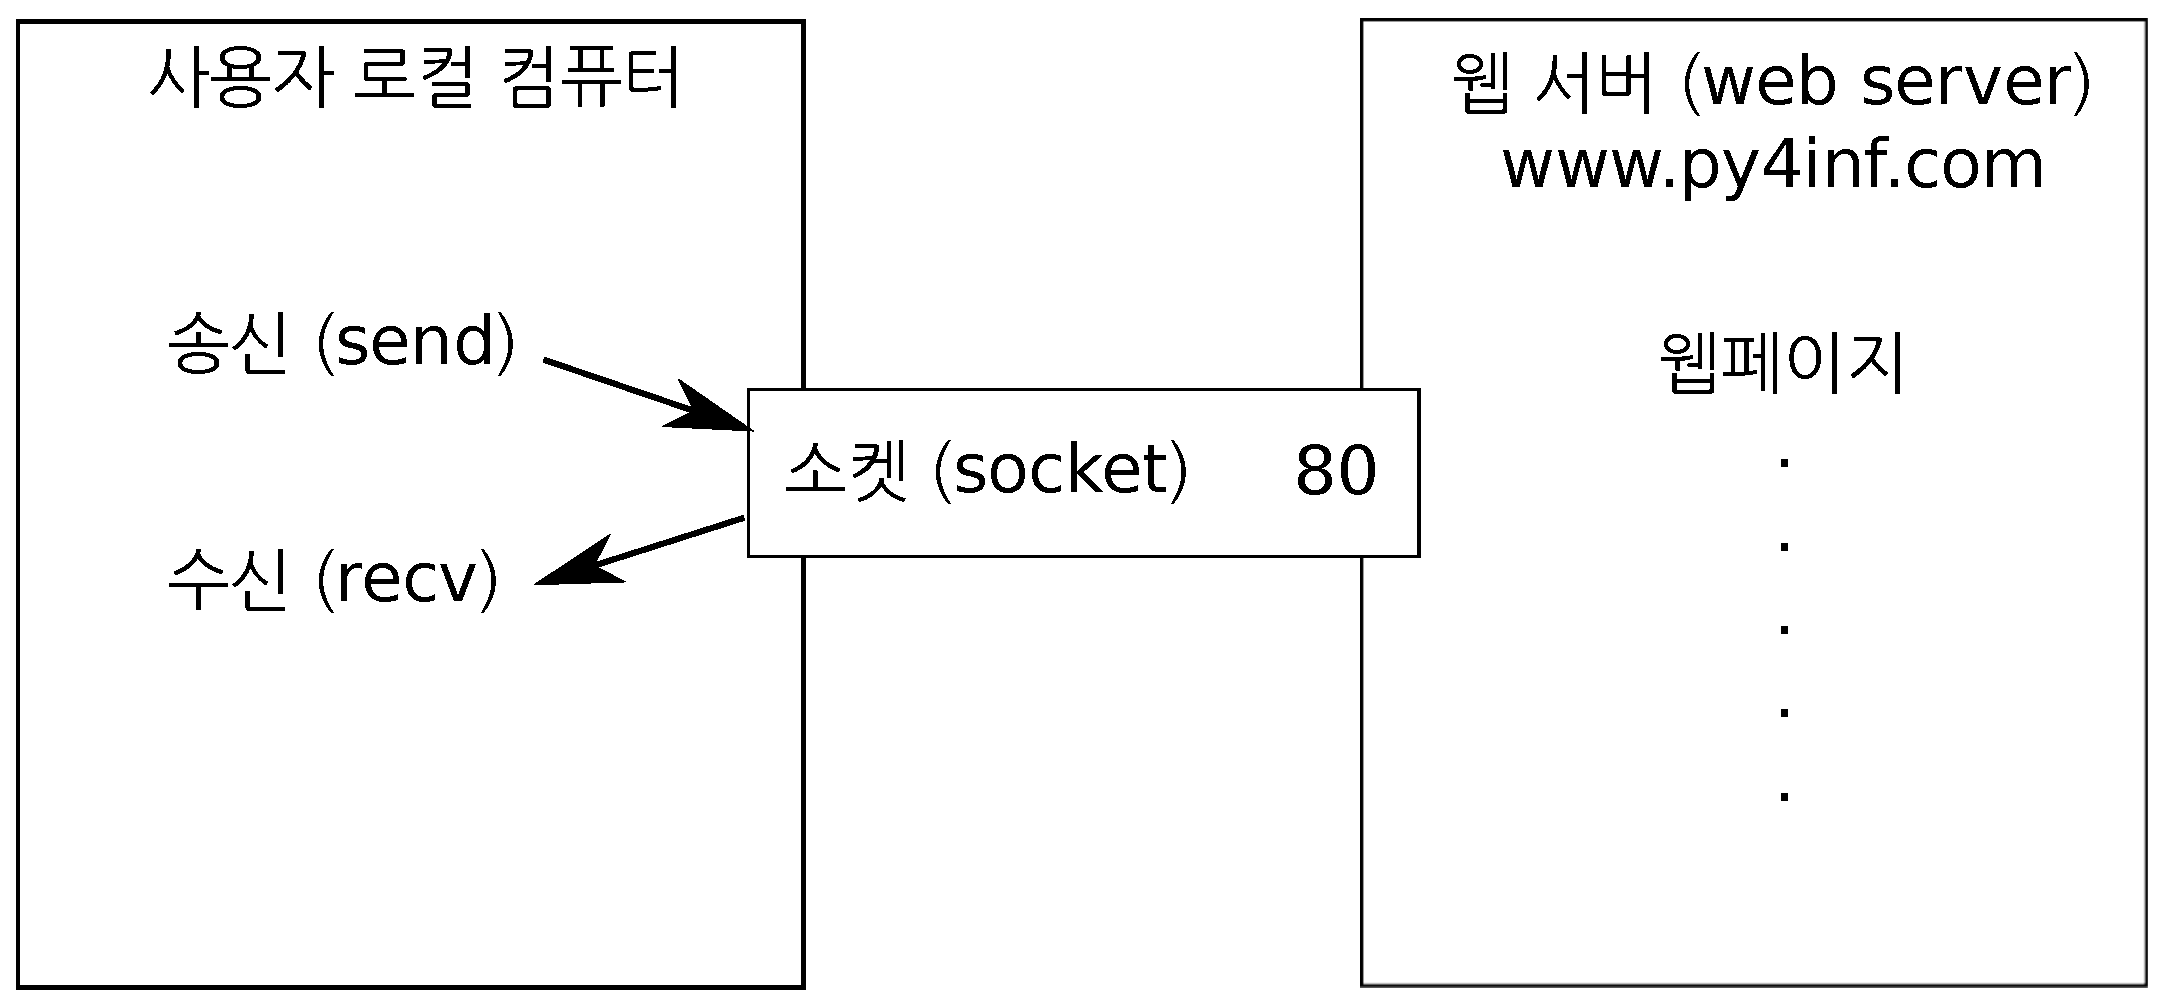
\includegraphics[height=1.50in]{figs2/socket.eps}}
\afterfig

공백 라인을 보내자 마자, 512 문자 덩어리의 데이터를 소켓에서 받아 더 이상 읽을 데이터가 없을 때까지(즉, recv()이 빈 문자열을 반환한다.) 데이터를 출력하는 루프를 작성한다.

프로그램 실행결과 다음을 얻을 수 있다.

\beforeverb
\begin{verbatim}
HTTP/1.1 200 OK
Date: Sun, 14 Mar 2010 23:52:41 GMT
Server: Apache
Last-Modified: Tue, 29 Dec 2009 01:31:22 GMT
ETag: "143c1b33-a7-4b395bea"
Accept-Ranges: bytes
Content-Length: 167
Connection: close
Content-Type: text/plain

But soft what light through yonder window breaks
It is the east and Juliet is the sun
Arise fair sun and kill the envious moon
Who is already sick and pale with grief
\end{verbatim}
\afterverb
%

출력결과는 웹서버가 문서를 기술하기 위해서 보내는 헤더(header)로 시작한다.
예를 들어, {\tt Content-Type } 헤더는 문서가 일반 텍스트 문서({\tt text/plain})임을 표기한다.

서버가 헤더를 보낸 후에, 빈 라인을 추가해서 헤더 끝임을 표기하고 나서 실제 파일{\tt romeo.txt}을 보낸다.

이 예제를 통해서 소켓을 통해서 저수준(low-level) 네트워크 연결을 어떻게 하는지 확인할 수 있다.
소켓을 사용해서 웹서버, 메일 서버 혹은 다른 종류의 서버와 통신할 수 있다.
필요한 것은 프로토콜을 기술하는 문서를 찾고 프로토콜에 따라 데이터를 주고 받는 코드를 작성하는 것이다.

하지만, 가장 흔히 사용하는 프로토콜은 HTTP (즉, 웹) 프로토콜이기 때문에, 
파이썬에는 HTTP 프로토컬을 지원하기 위해 특별히 설계된 라이브러리가 있다.
이것을 통해서 웹상에서 데이터나 문서를 검색을 쉽게 할 수 있다.

\section{HTTP를 통해서 이미지 가져오기}

\index{urllib!이미지 (image)}
\index{이미지 (image)!jpg}
\index{jpg}

상기 예제에서는 파일에 새줄(newline)이 있는 일반 텍스트 파일을 가져왔다. 
그리고 나서, 프로그램을 실행해서 데이터를 단순히 화면에 복사했다.
HTTP를 사용하여 이미지를 가져오도록 비슷하게 프로그램을 작성할 수 있다. 
프로그램 실행 시에 화면에 데이터를 복사하는 대신에,
데이터를 문자열로 누적하고, 다음과 같이 헤더를 잘라내고 나서 파일에 이미지 데이터를 저장한다. 

\beforeverb
\begin{verbatim}
import socket
import time

mysock = socket.socket(socket.AF_INET, socket.SOCK_STREAM)
mysock.connect(('www.py4inf.com', 80))
mysock.send('GET http://www.py4inf.com/cover.jpg HTTP/1.0\n\n')


count = 0
picture = "";
while True:
    data = mysock.recv(5120)
    if ( len(data) < 1 ) : break
    # time.sleep(0.25)
    count = count + len(data)
    print len(data),count
    picture = picture + data

mysock.close()

# Look for the end of the header (2 CRLF)
pos = picture.find("\r\n\r\n");
print 'Header length',pos
print picture[:pos]

# Skip past the header and save the picture data
picture = picture[pos+4:]
fhand = open("stuff.jpg","wb")
fhand.write(picture);
fhand.close()
\end{verbatim}
\afterverb
%

프로그램을 실행하면, 다음과 같은 출력을 생성한다.

\beforeverb
\begin{verbatim}
$ python urljpeg.py 
2920 2920
1460 4380
1460 5840
1460 7300
...
1460 62780
1460 64240
2920 67160
1460 68620
1681 70301
Header length 240
HTTP/1.1 200 OK
Date: Sat, 02 Nov 2013 02:15:07 GMT
Server: Apache
Last-Modified: Sat, 02 Nov 2013 02:01:26 GMT
ETag: "19c141-111a9-4ea280f8354b8"
Accept-Ranges: bytes
Content-Length: 70057
Connection: close
Content-Type: image/jpeg
\end{verbatim}
\afterverb
%
상기 url에 대해서, {\tt Content-Type } 헤더가 문서 본문이 이미지({\tt image/jpeg})를 나타내는 것을 볼 수 있다.
프로그램이 완료되면, 이미지 뷰어로 {\tt stuff.jpg} 파일을 열어서 이미지 데이터를 볼 수 있다.

프로그램을 실행하면, {\tt recv()} 메쏘드를 호출할 때 마다 5120 문자는 전달받지 못하는 것을 볼 수 있다.
{\tt recv()} 호출하는 순간마다 웹서버에서 네트워크로 전송되는 가능한 많은 문자를 받을 뿐이다. 
매번 5120 문자까지 요청하지만, 1460 혹은 2920 문자만 전송받는다. 

결과값은 네트워크 속도에 따라 달라질 수 있다. 
{\tt recv()} 메쏘드 마지막 호출에는 스트림 마지막인 1681 바이트만 받았고,
{\tt recv()} 다음 호출에는 0 길이 문자열을 전송받아서, 서버가 소켓 마지막에 {\tt close()} 메쏘드를 호출하고 
더이상의 데이터가 없다는 신호를 준다.

\index{시간 (time)}
\index{정지 시간 (time.sleep)}

주석 처리한 {\tt time.sleep()}을 풀어줌으로써 {\tt recv()} 연속 호출을 늦출 수 있다.
이런 방식으로 매번 호출 후에 0.25초 기다리게 한다.
그래서, 사용자가 {\tt recv()} 메쏘드를 호출하기 전에 서버가 먼저 도착할 수 있어서 더 많은 데이터를 보낼 수가 있다.
정지 시간을 넣어서 프로그램을 다시 실행하면 다음과 같다.

\beforeverb
\begin{verbatim}
$ python urljpeg.py 
1460 1460
5120 6580
5120 11700
...
5120 62900
5120 68020
2281 70301
Header length 240
HTTP/1.1 200 OK
Date: Sat, 02 Nov 2013 02:22:04 GMT
Server: Apache
Last-Modified: Sat, 02 Nov 2013 02:01:26 GMT
ETag: "19c141-111a9-4ea280f8354b8"
Accept-Ranges: bytes
Content-Length: 70057
Connection: close
Content-Type: image/jpeg
\end{verbatim}
\afterverb
%

{\tt recv()} 메쏘드 호출의 처음과 마지막을 제외하고, 매번 새로운 데이터를 요청할 때마다 이제 5120 문자가 전송된다.

서버 {\tt send()} 요청과 응용프로그램 {\tt recv()} 요청 사이에 버퍼가 있다.
프로그램에 지연을 넣어 실행하게 될 때, 어느 지점엔가 서버가 소켓 버퍼를 채우고 응용프로그램이 버퍼를 비울 때까지 잠시 멈춰야 된다. 
송신하는 응용프로그램 혹은 수신하는 응용프로그램을 멈추게 하는 행위를 ''흐름 제어(flow control)''이라고 한다.

\index{흐름 제어 (flow control)}

\section{{\tt urllib} 사용하여 웹페이지 가져오기}

수작업으로 소켓 라이브러리를 사용하여 HTTP로 데이터를 주고 받을 수 있지만,
{\tt urllib} 라이브러리를 사용하여 파이썬에서 동일한 작업을 수행하는 좀더 간편한 방식이 있다.

{\tt urllib}을 사용하여 파일처럼 웹페이지를 다룰 수가 있다.
단순하게 어느 웹페이지를 가져올 것인지만 지정하면 {\tt urllib} 라이브러리가 모든 HTTP 프로토콜과 헤더관련 사항을 처리해 준다.

웹에서 {\tt romeo.txt} 파일을 읽도록 {\tt urllib}를 사용하여 작성한 상응 코드는 다음과 같다.

\beforeverb
\begin{verbatim}
import urllib

fhand = urllib.urlopen('http://www.py4inf.com/code/romeo.txt')
for line in fhand:
   print line.strip()
\end{verbatim}
\afterverb
%

{\tt urllib.urlopen}을 사용하여 웹페이지를 열게 되면, 파일처럼 다룰 수 있고 {\tt for} 루프를 사용하여 데이터를 읽을 수 있다.

프로그램을 실행하면, 파일 내용 출력결과만을 볼 수 있다. 
헤더정보는 여전히 전송되었지만, {\tt urllib} 코드가 헤더를 받아 내부적으로 처리하고, 사용자에게는 단지 데이터만 반환한다.

\beforeverb
\begin{verbatim}
But soft what light through yonder window breaks
It is the east and Juliet is the sun
Arise fair sun and kill the envious moon
Who is already sick and pale with grief
\end{verbatim}
\afterverb
%

예제로, {\tt romeo.txt} 데이터를 가져와서 파일의 각 단어 빈도를 계산하는 프로그램을 다음과 같이 작성할 수 있다.

\beforeverb
\begin{verbatim}
import urllib

counts = dict()
fhand = urllib.urlopen('http://www.py4inf.com/code/romeo.txt')
for line in fhand:
    words = line.split()
    for word in words:
        counts[word] = counts.get(word,0) + 1   
print counts
\end{verbatim}
\afterverb
%

다시 한번, 웹페이지를 열게 되면, 로컬 파일처럼 웹페이지를 읽을 수 있다.

\section{HTML 파싱과 웹 스크래핑}

\index{웹 (web)!스크래핑 (scraping)}
\index{HTML 피싱 (parsing HTML)}

파이썬 {\tt urllib} 활용하는 일반적인 사례는 웹 {\bf 스크래핑(scraping)}이다.
웹 스크래핑은 웹브라우저를 가장한 프로그램을 작성하는 것이다.
웹페이지를 가져와서, 패턴을 찾아 페이지 내부의 데이터를 꼼꼼히 조사한다.
예로, 구글같은 검색엔진은 웹 페이지의 소스를 조사해서 다른 페이지로 가는 링크를 추출하고, 그 해당 페이지를 가져와서 링크 추출하는 작업을 반복한다.
이러한 기법으로 구글은 웹상의 거의 모든 페이지를 {\bf 거미(spiders)}줄처럼 연결한다.

구글은 또한 발견한 웹페이지에서 특정 페이지로 연결되는 링크 빈도를 사용하여 얼마나 중요한 페이지인지를 측정하고 
검색결과에 페이지가 얼마나 높은 순위로 노출되어야 하는지 평가한다.

\section{정규 표현식 사용 HTML 파싱하기}

HTML을 파싱하는 간단한 방식은 정규 표현식을 사용하여 특정한 패턴과 매칭되는 부속 문자열을 반복적으로 찾아 추출하는 것이다.

여기 간단한 웹페이지가 있다.

\beforeverb
\begin{verbatim}
<h1>The First Page</h1>
<p>
If you like, you can switch to the
<a href="http://www.dr-chuck.com/page2.htm">
Second Page</a>.
</p>
\end{verbatim}
\afterverb
%

모양 좋은 정규표현식을 구성해서 다음과 같이 상기 웹페이지에서 링크를 매칭하고 추출할 수 있다.

\beforeverb
\begin{verbatim}
href="http://.+?"
\end{verbatim}
\afterverb
%


작성된 정규 표현식은 ``href="http://''로 시작하고, 하나 이상의 문자를 ``.+?'' 가지고 큰 따옴표를 가진 문자열을 찾는다.
``.+?''에 물음표가 갖는 의미는 매칭이 ''욕심쟁이(greedy)'' 방식보다 ''비욕심쟁이(non-greedy)'' 방식으로 수행됨을 나타낸다. 
비욕심쟁이(non-greedy) 매칭방식은 가능한 \emph{가장 적게} 매칭되는 문자열을 찾는 방식이고, 욕심 방식은 가능한 \emph{가장 크게} 매칭되는 문자열을 찾는 방식이다.

\index{욕심쟁이 (greedy)}
\index{비욕심쟁이 (non-greedy)}

추출하고자 하는 문자열이 매칭된 문자열의 어느 부분인지를 표기하기 위해서 정규 표현식에 괄호를 추가하여 다음과 같이 프로그램을 작성한다.

\index{정규 표현식 (regex)!괄호 (parentheses)}
\index{괄호 (parentheses)!정규 표현식 (regular expression)}

\beforeverb
\begin{verbatim}
import urllib
import re

url = raw_input('Enter - ')
html = urllib.urlopen(url).read()
links = re.findall('href="(http://.*?)"', html)
for link in links:
    print link
\end{verbatim}
\afterverb
%

{\tt findall} 정규 표현식 메쏘드는 정규 표현식과 매칭되는 모든 문자열 리스트를 추출하여 큰 따옴표 사이에 링크 텍스트만을 반환한다.

프로그램을 실행하면, 다음 출력을 얻게된다.

\beforeverb
\begin{verbatim}
python urlregex.py 
Enter - http://www.dr-chuck.com/page1.htm
http://www.dr-chuck.com/page2.htm

python urlregex.py 
Enter - http://www.py4inf.com/book.htm
http://www.greenteapress.com/thinkpython/thinkpython.html
http://allendowney.com/
http://www.py4inf.com/code
http://www.lib.umich.edu/espresso-book-machine
http://www.py4inf.com/py4inf-slides.zip
\end{verbatim}
\afterverb
%

정규 표현식은 HTML이 예측가능하고 잘 구성된 경우에 멋지게 작동한다.
하지만, ''망가진'' HTML 페이지가 많아서, 정규 표현식만을 사용하는 솔류션은 유효한 링크를 놓치거나 잘못된 데이터만 찾고 끝날 수 있다.

이 문제는 강건한 HTML 파싱 라이브러리를 사용해서 해결될 수 있다.

\section{BeautifulSoup 사용한 HTML 파싱}
\index{뷰티풀수프 (BeautifulSoup)}

HTML을 파싱하여 페이지에서 데이터를 추출할 수 있는 파이썬 라이브러리는 많이 있다.
라이브러리 각각은 강점과 약점이 있어서 사용자 필요에 따라 취사선택한다.

예로, 간단하게 HTML 입력을 파싱하여 {\bf BeautifulSoup} 라이브러리를 사용하여 링크를 추출할 것이다.
다음 웹사이트에서 BeautifulSoup 코드를 다운로드 받아 설치할 수 있다.

\url{www.crummy.com}

BeautifulSoup 라이브러리를 다운로드 받아 ''설치''하거나 {\tt BeautifulSoup.py} 파일을 응용프로그램과 동일한 폴더에 저장한다.

HTML이 XML 처럼 보이고 몇몇 페이지는 XML로 되도록 꼼꼼하게 구축되었지만, 
일반적으로 대부분의 HTML이 깨져서 XML 파서가 HTML 전체 페이지를 잘못 구성된 것으로 간주하고 받아들이지 않는다.
BeautifulSoup 라이브러리는 결점 많은 HTML 페이지에 내성이 있어서 사용자가 필요로하는 데이터를 쉽게 추출할 수 있게 한다.

{\tt urllib}를 사용하여 페이지를 읽어들이고, {\tt BeautifulSoup}를 사용해서 앵커 태그 ({\tt a})로부터 {\tt href} 속성을  추출한다.

\index{뷰티풀수프 (BeautifulSoup)}
\index{HTML}
\index{파싱 (parsing)!HTML}

\beforeverb
\begin{verbatim}
import urllib
from BeautifulSoup import *

url = raw_input('Enter - ')
html = urllib.urlopen(url).read()
soup = BeautifulSoup(html)

# Retrieve all of the anchor tags
tags = soup('a')
for tag in tags:
   print tag.get('href', None)
\end{verbatim}
\afterverb
%

프로그램이 웹 주소를 입력받고, 웹페이지를 열고, 데이터를 읽어서 BeautifulSoup 파서에 전달하고,
그리고 나서 모든 앵커 태그를 불러와서 각 태그별로 {\tt href} 속성을 출력한다.

프로그램을 실행하면, 아래와 같다.

\beforeverb
\begin{verbatim}
python urllinks.py 
Enter - http://www.dr-chuck.com/page1.htm
http://www.dr-chuck.com/page2.htm

python urllinks.py 
Enter - http://www.py4inf.com/book.htm
http://www.greenteapress.com/thinkpython/thinkpython.html
http://allendowney.com/
http://www.si502.com/
http://www.lib.umich.edu/espresso-book-machine
http://www.py4inf.com/code
http://www.pythonlearn.com/
\end{verbatim}
\afterverb
%

BeautifulSoup을 사용하여 다음과 같이 각 태그별로 다양한 부분을 뽑아낼 수 있다.

\beforeverb
\begin{verbatim}
import urllib
from BeautifulSoup import *

url = raw_input('Enter - ')
html = urllib.urlopen(url).read()
soup = BeautifulSoup(html)

# Retrieve all of the anchor tags
tags = soup('a')
for tag in tags:
   # Look at the parts of a tag
   print 'TAG:',tag
   print 'URL:',tag.get('href', None)
   print 'Content:',tag.contents[0]
   print 'Attrs:',tag.attrs
\end{verbatim}
\afterverb
%

상기 프로그램은 다음을 출력합니다.

\beforeverb
\begin{verbatim}
python urllink2.py 
Enter - http://www.dr-chuck.com/page1.htm
TAG: <a href="http://www.dr-chuck.com/page2.htm">
Second Page</a>
URL: http://www.dr-chuck.com/page2.htm
Content: [u'\nSecond Page']
Attrs: [(u'href', u'http://www.dr-chuck.com/page2.htm')]
\end{verbatim}
\afterverb
%

HTML을 파싱하는데 BeautifulSoup이 가진 강력한 기능을 예제로 보여줬다.
좀더 자세한 사항은 \url{www.crummy.com} 에서 문서와 예제를 살펴보세요.

\section{urllib을 사용하여 바이너리 파일 읽기}

이미지나 비디오 같은 텍스트가 아닌 (혹은 바이너리) 파일을 가져올 때가 종종 있다.
일반적으로 이런 파일 데이터를 출력하는 것은 유용하지 않다. 
하지만, {\tt urllib}을 사용하여, 하드 디스크 로컬 파일에 URL 사본을 쉽게 만들 수 있다.

\index{바이너리 파일 (binary file)}

이 패턴은 URL을 열고, {\tt read}를 사용해서 문서 전체 내용을 다운로드하여 문자열 변수({\tt img})에 다운로드하고,
그리고 나서 다음과 같이 정보를 로컬 파일에 쓴다.

\beforeverb
\begin{verbatim}
img = urllib.urlopen('http://www.py4inf.com/cover.jpg').read()
fhand = open('cover.jpg', 'w')
fhand.write(img)
fhand.close()
\end{verbatim}
\afterverb
%

작성된 프로그램은 네트워크로 모든 데이터를 한번에 읽어서 컴퓨터 주기억장치 {\tt img} 변수에 저장하고,
{\tt cover.jpg} 파일을 열어 디스크에 데이터를 쓴다. 
이 방식은 파일 크기가 사용자 컴퓨터의 메모리 크기보다 작다면 정상적으로 작동한다.

하지만, 오디오 혹은 비디오 파일 대용량이면, 상기 프로그램은 멈추거나 사용자 컴퓨터 메모리가 부족할 때 극단적으로 느려질 수 있다.
메모리 부족을 회피하기 위해서, 데이터를 블럭 혹은 버퍼로 가져와서, 다음 블럭을 가져오기 전에 디스크에 각각의 블럭을 쓴다.
이런 방식으로 사용자가 가진 모든 메모리를 사용하지 않고 어떠한 크기 파일도 읽어올 수 있다.

\beforeverb
\begin{verbatim}
import urllib

img = urllib.urlopen('http://www.py4inf.com/cover.jpg')
fhand = open('cover.jpg', 'w')
size = 0
while True:
    info = img.read(100000)
    if len(info) < 1 : break
    size = size + len(info)
    fhand.write(info)

print size,'characters copied.'
fhand.close()
\end{verbatim}
\afterverb
%

상기 예제에서, 한번에 100,000 문자만 읽어 오고, 웹에서 다음 100,000 문자를 가져오기 전에 {\tt cover.jpg} 파일에 읽어온 문자를 쓴다.

프로그램 실행 결과는 다음과 같다.

\beforeverb
\begin{verbatim}
python curl2.py 
568248 characters copied.
\end{verbatim}
\afterverb
%

UNIX 혹은 매킨토시 컴퓨터를 가지고 있다면, 다음과 같이 상기 동작을 수행하는 명령어가 운영체제 자체에 내장되어 있다.

\index{curl}

\beforeverb
\begin{verbatim}
curl -O http://www.py4inf.com/cover.jpg
\end{verbatim}
\afterverb
%

{\tt curl}은 ``copy URL''의 단축 명령어로 두 예제는 {\tt curl} 명령어와 비슷한 기능을 구현해서, 
\url{www.py4inf.com/code} 사이트에 {\tt curl1.py}, {\tt curl2.py} 이름으로 올라가 있다.
동일한 작업을 좀더 효과적으로 수행하는 {\tt curl3.py} 샘플 프로그램도 있어서 실무적으로 작성하는 프로그램에 이런한 패턴을 이용하여 구현할 수 잇다.

\section{용어정의}

\begin{description}

\item[BeautifulSoup:] 파이썬 라이브러리로 HTML 문서를 파싱하고 
브라우저가 일반적으로 생략하는 HTML의 불완전한 부분을 보정하여 HTML 문서에서 데이터를 추출한다.
\url{www.crummy.com} 사이트에서 BeautifulSoup 코드를 다운로드 받을 수 있다.
\index{뷰티풀수프 (BeautifulSoup)}

\item[포트(port):] 서버에 소켓 연결을 만들 때, 사용자가 무슨 응용프로그램을 연결하는지 나타내는 숫자.
예로, 웹 트래픽은 통상 80 포트, 전자우편은 25 포트를 사용한다.
\index{포트 (port)}

\item[스크래핑(scraping):] 프로그램이 웹브라우저를 가장하여 웹페이지를 가져와서 웹 페이지의 내용을 검색한다.
종종 프로그램이 한 페이지의 링크를 따라 다른 페이지를 찾게 된다. 그래서, 웹페이지 네트워크 혹은 소셜 네트워크 전체를 훑을 수 있다.
\index{스크래핑 (scraping}

\item[소켓(socket):] 두 응용프로그램 사이 네트워크 연결. 두 응용프로그램은 양 방향으로 데이터를 주고 받는다.
\index{소켓 (socket)}

\item[스파이더(spider):] 검색 색인을 구축하기 위해서 한 웹페이지를 검색하고, 그 웹페이지에 링크된 모든 페이지 검색을 반복하여
인터넷에 있는 거의 모든 웹페이지를 가져오기 위해서 사용되는 검색엔진 행동.
\index{스파이더 (spider)}

\end{description}

\section{연습문제}

\begin{ex}
소켓 프로그램 {\tt socket1.py}을 변경하여 임의 웹페이지를 읽을 수 있도록 URL을 사용자가 입력하도록 바꾸세요.
{\tt split('/')}을 사용하여 URL을 컴포턴트로 쪼개서 소켓 {\tt connect} 호출에 대해 호스트 명을 추출할 수 있다.
사용자가 적절하지 못한 형식 혹은 존재하지 않는 URL을 입력하는 경우를 처리할 있도록 {\tt try}, {\tt except}를 사용하여 오류 검사기능을 추가하세요.
\end{ex}

\begin{ex}
소켓 프로그램을 변경하여 전송받은 문자를 계수(count)하고 3000 문자를 출력한 후에 그이상 텍스트 출력을 멈추게 하세요.
프로그램은 전체 문서를 가져와야 하고, 전체 문자를 계수(count)하고, 문서 마지막에 문자 계수(count)결과를 출력해야 합니다.
\end{ex}

\begin{ex}
{\tt urllib}을 사용하여 이전 예제를 반복하세요. (1) 사용자가 입력한 URL에서 문서 가져오기
(2) 3000 문자까지 화면에 보여주기 (3) 문서의 전체 문자 계수(count)하기.
이 연습문제에서 헤더에 대해서는 걱정하지 말고, 단지 문서 본문에서 첫 3000 문자만 화면에 출력하세요.
\end{ex}

\begin{ex} {\tt urllinks.py} 프로그램을 변경하여 가져온 HTML 문서에서 문단 (p) 태그를 추출하고
프로그램의 출력물로 문단을 계수(count)하고 화면에 출력하세요. 
문단 텍스트를 화면에 출력하지 말고 단지 숫자만 셉니다.
작성한 프로그램을 작은 웹페이지 뿐만 아니라 조금 큰 웹 페이지에도 테스트해 보세요.
\end{ex}

\begin{ex}
(고급) 소켓 프로그램을 변경하여 헤더와 빈 라인 다음에 데이터만 보여지게 하세요.
{\tt recv}는 라인이 아니라 문자(새줄(newline)과 모든 문자)를 전송받는다는 것을 기억하세요.
\end{ex}



\input{13-web}
% The contents of this file is 
% Copyright (c) 2009-  Charles R. Severance, All Righs Reserved

\chapter{데이터베이스와 SQL(Structured Query Language) 사용하기}

\section{데이터베이스가 뭔가요?}
\index{데이터베이스 (database)}

{\bf 데이터베이스(database)}는 데이터를 저장하기 위한 목적으로 조직된 파일이다. 
대부분의 데이터베이스는 키(key)와 값(value)를 매핑한다는 의미에서 딕셔너리처럼 조직되었다.
가장 큰 차이점은 데이터베이스는 디스크(혹은 다른 영구 저장소)에 위치하고 있어서, 프로그램 종료 후에도 정보가 계속 저장된다.
데이터베이스가 영구 저장소에 저장되어서, 컴퓨터 주기억장치(memory) 크기에 제한받는 딕셔너리보다 훨씬 더 많은 정보를 저장할 수 있다.

\index{데이터베이스 (database)!인덱스 (indexes)}

딕셔너리처럼, 데이터베이스 소프트웨어는 엄청난 양의 데이터 조차도 매우 빠르게 삽입하고 접근하도록 설계되었다.
컴퓨터가 특정 항목으로 빠르게 찾아갈 수 있도록 데이터베이스에 {\bf 인덱스(indexes)}를 추가한다.
데이터베이스 소프트웨어는 인덱스를 구축하여 성능을 보장한다.

다양한 목적에 맞춰 서로 다른 많은 데이터베이스 시스템이 개발되어 사용되고 있다. 
Oracle, MySQL, Microsoft SQL Server, PostgreSQL, SQLite이 여기에 포함된다. 
이 책에서는 SQLite를 집중해서 살펴볼 것이다. 
왜냐하면 매우 일반적인 데이터베이스이며 파이썬에 이미 내장되어 있기 때문이다.
응용프로그램 내부에서 데이터베이스 기능을 제공하도록 SQLite가 다른 응용프로그램 내부에 \emph{내장(embedded)}되도록 설계되었다.
예를 들어, 다른 많은 소프트웨어 제품이 그렇듯이, 파이어폭스 브라우져도 SQLite를 사용한다.

\url{http://sqlite.org/}

이번 장에서 기술하는 트위터 스파이더링 응용프로그램처럼 정보과학(Informatics)에서 마주치는 몇몇 데이터 조작 문제에 SQLite가 적합하다.


\section{데이터베이스 개념}
처음 데이터베이스를 볼때 드는 생각은 마치 엑셀같은 다중 시트를 지닌 스프레드쉬트(spreadsheet)같다는 것이다.
데이터베이스에서 주요 데이터 구조물은 {\bf 테이블(tables)}, {\bf 행(rows)}, and {\bf 열(columns)}이 된다. 

\beforefig
\centerline{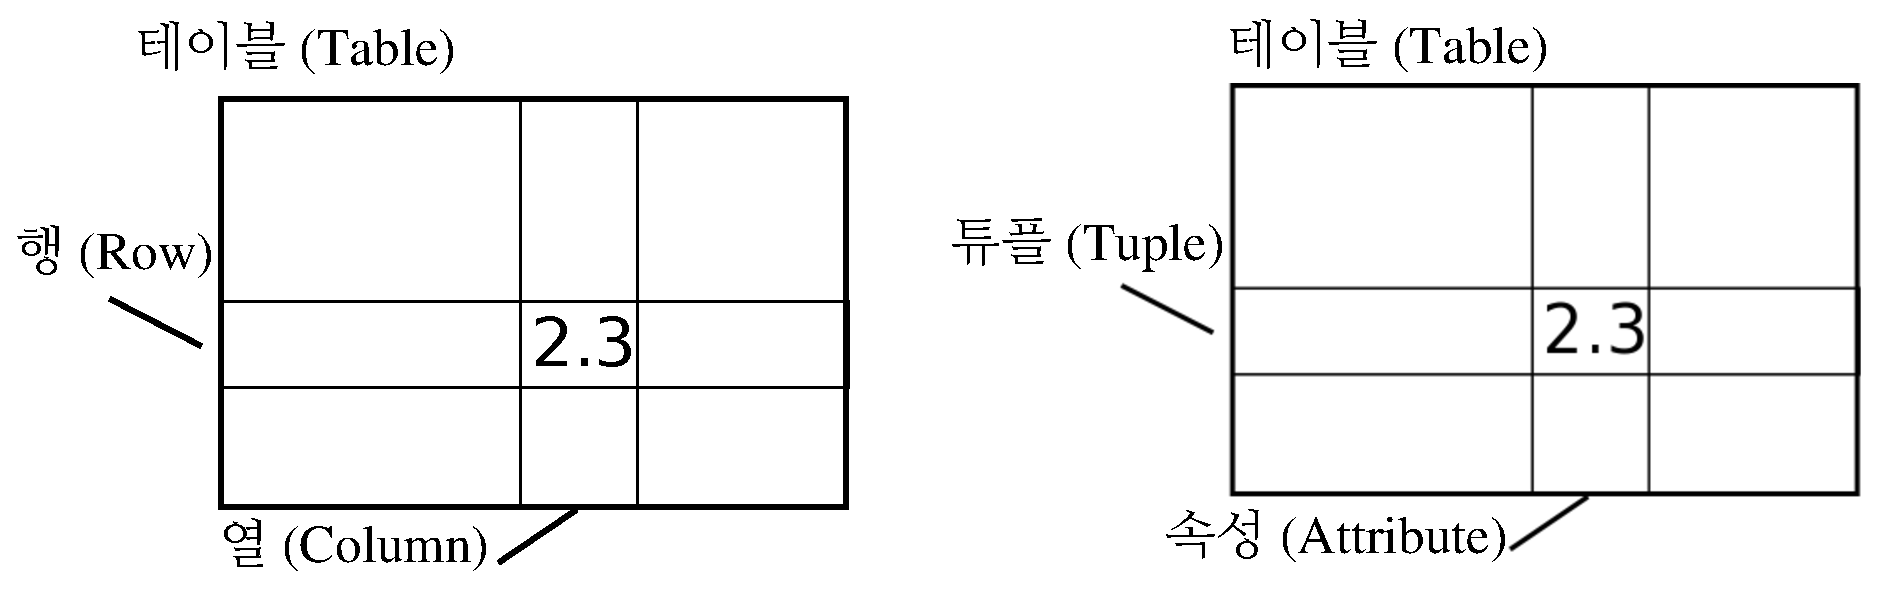
\includegraphics[height=1.50in]{figs2/relational.eps}}
\afterfig

관계형 데이터베이스의 기술적인 면을 설명하면 테이블, 행, 열의 개념은 
{\bf 관계(relation)}, {\bf 튜플(tuple)}, and {\bf 속성(attribute)} 각각 형식적으로 매칭된다.
이번 장에서는 조금 덜 형식 용어를 사용한다.

\section{파이어폭스 애드온 SQLite 매니저}
SQLite 데이터베이스 파일에 있는 데이터를 다루기 위해서 이번장에서 주로 파이썬 사용에 집중을 하지만, 
다음 웹사이트에서 무료로 이용 가능한 {\bf SQLite 데이터베이스 매니저(SQLite Database Manager)}로 불리는 
파이어폭스 애드온(add-on)을 사용해서 좀더 쉽게 많은 작업을 수행할 수 있다.

\url{https://addons.mozilla.org/en-us/firefox/addon/sqlite-manager/}

브라우져를 사용해서 쉽게 테이블을 생성하고, 데이터를 삽입, 편집하고 데이터베이스 데이터에 대해 간단한 SQL 질의를 실행할 수 있다.

이러한 점에서 데이터베이스 매니저는 텍스트 파일을 작업할 때 사용하는 텍스트 편집기와 유사하다.
텍스트 파일에 하나 혹은 몇개 작업만 수행하고자 하면, 텍스트 편집기에서 파일을 열어 필요한 수정작업을 하고 닫으면 된다.
텍스트 파일에 작업할 사항이 많은 경우는 종종 간단한 파이썬 프로그램을 작성하여 수행한다.
데이터베이스로 작업할 때도 동일한 패턴이 발견된다. 
간단한 작업은 데이터베이스 매니저를 통해서 수행하고,
좀더 복잡한 작업은 파이썬으로 수행하는 것이 더 편리하다.


\section{데이터베이스 테이블 생성하기}

데이터베이스는 파이썬 리스트 혹은 딕셔너리보다 좀더 명확히 정의된 구조를 요구한다.\footnote{
실질적으로 SQLite는 열에 저장되는 데이터 형식에 대해서 좀더 많은 유연성을 부여하지만,
이번 장에서는 데이터 형식을 엄격하게 적용해서 MySQL 같은 다른 관계형 데이터베이스 시스템에도 동일한 개념이 적용되게 한다.}.  

데이터베이스에 {\bf 테이블(table)}을 생성할 때, {\bf 열(column)}의 명칭과 각 {\bf 열(column)}에 저장하는 테이터 형식을 사전에 정의해야 한다. 
데이터베이스 소프트웨어가 각 열의 데이터 형식을 인식하게 되면, 데이터 형식에 따라 데이터를 저장하고 찾아오는 방법을 가장 효율적인 방식을 선택할 수 있다.

다음 url에서 SQLite에서 지원되는 다양한 데이터 형식을 살펴볼 수 있다.

\url{http://www.sqlite.org/datatypes.html}

처음에는 데이터 구조를 사전에 정의하는 것이 불편하게 보이지만, 대용량의 데이터가 데이터베이스에 포함되더라도 데이터의 빠른 접근을 보장하는 잇점이 있다.

데이터베이스 파일과 데이터베이스에 두개의 열을 가진 {\tt Tracks} 이름의 테이블을 생성하는 코드는 다음과 같다.

\index{sqlite3 module}
\index{module!sqlite3}
\beforeverb
\begin{verbatim}
import sqlite3

conn = sqlite3.connect('music.sqlite3')
cur = conn.cursor()

cur.execute('DROP TABLE IF EXISTS Tracks ')
cur.execute('CREATE TABLE Tracks (title TEXT, plays INTEGER)')

conn.close()
\end{verbatim}
\afterverb
%

\index{연결 함수 (connect function)}
\index{함수 (function)!연결 (connect)}
\index{커서 함수 (cursor function)}
\index{함수 (function)!커서 (cursor)}

{\tt 연결 (connect)} 연산은 현재 디렉토리 {\tt music.sqlite3} 파일에 저장된 데이터베이스에 ''연결(connection)''한다.
파일이 존재하지 않으면, 자동 생성된다. 
''연결(connection)''이라고 부르는 이유는 때때로 데이터베이스가 응용프로그램이 실행되는 서버로부터
분리된 ''데이터베이스 서버(database server)''에 저장되기 때문이다.
지금 간단한 예제 파일의 경우에 데이터베이스가 로컬 파일 형태로 파이썬 코드 마찬가지로 동일한 디렉토리에 있다.

파일을 다루는 파일 핸들(file handle)처럼 데이터베이스에 저장된 파일에 연산을 수행하기 위해서 {\bf 커서(cursor)}를 사용한다.
{\tt cursor()}를 호출하는 것은 개념적으로 텍스트 파일을 다룰 때 {\tt open()}을 호출하는 것과 개념적으로 매우 유사하다.

\beforefig
\centerline{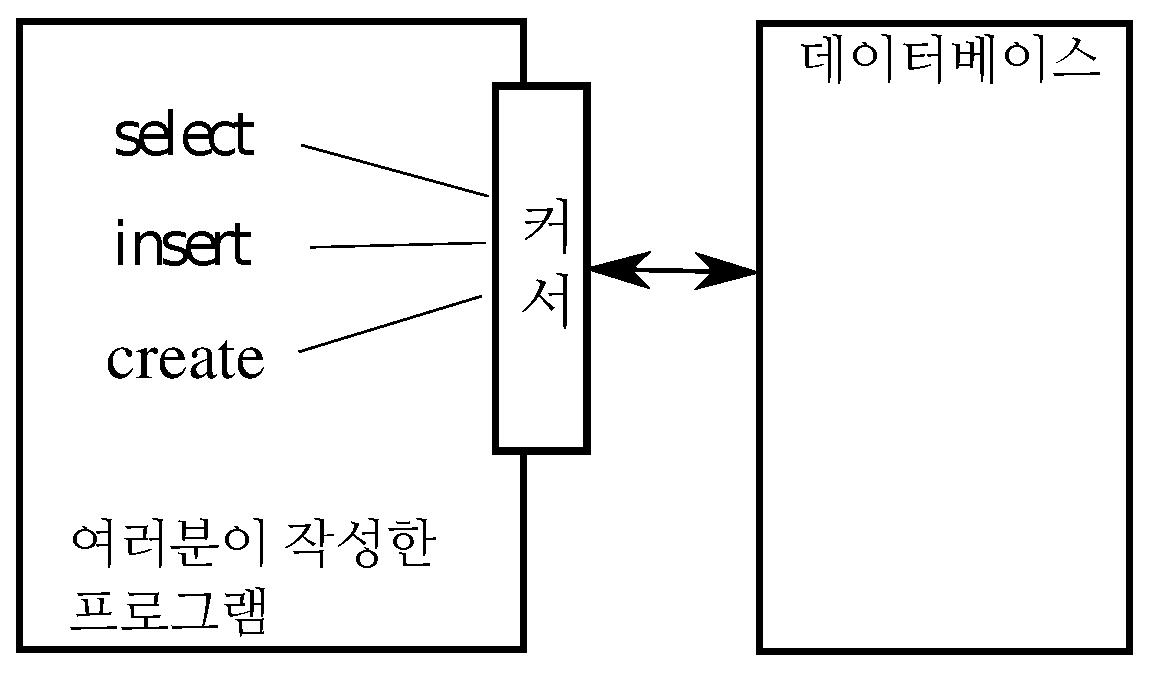
\includegraphics[height=1.50in]{figs2/cursor.eps}}
\afterfig

커서가 생성되면, {\tt execute()} 메쏘드를 사용하여 데이터베이스 콘텐츠에 명령어 실행을 할 수 있다.

데이터베이스 명령어는 특별한 언어로 표현된다.
단일 데이터베이스 언어를 학습하도록 서로 다른 많은 데이터베이스 업체 사이에서 표준화되었다.

데이터베이스 언어를 {\bf SQL(Structured Query Language 구조적 질의 언어)}로 부른다.

\url{http://en.wikipedia.org/wiki/SQL}

상기 예제에서, 데이터베이스에 두개의 SQL 명령어를 실행했다. 
관습적으로 데이터베이스 키워드는 대문자로 표기한다.
테이블명이나 열의 명칭처럼 사용자가 추가한 명령어 부분은 소문자로 표기한다.

첫 SQL 명령어는 만약 존재한다면 데이터베이스에서 {\tt Tracks} 테이블을 삭제한다.
동일한 프로그램을 실행해서 오류 없이 반복적으로 {\tt Tracks} 테이블을 생성하도록하는 패턴이다.
{\tt DROP TABLE} 명령어는 데이터베이스 테이블 및 테이블 콘텐츠 전부를 삭제하니 주의한다. (즉, ''실행취소(undo)''가 없다.)

\beforeverb
\begin{verbatim}
cur.execute('DROP TABLE IF EXISTS Tracks ')
\end{verbatim}
\afterverb
%

두번째 명령어는 {\tt title} 문자형 열과 {\tt plays} 정수형 열을 가진 {\tt Tracks}으로 명명된 테이블을 생성한다.

\beforeverb
\begin{verbatim}
cur.execute('CREATE TABLE Tracks (title TEXT, plays INTEGER)')
\end{verbatim}
\afterverb
%

이제 {\tt Tracks}으로 명명된 테이블을 생성했으니, SQL {\tt INSERT} 연산을 통해 테이블에 데이터를 넣을 수 있다.
다시 한번, 데이터베이스에 연결하여 {\tt 커서(cursor)}를 얻어 작업을 시작한다. 
그리고 나서 커서를 사용해서 SQL 명령어를 수행한다.

SQL {\tt INSERT} 명령어는 어느 테이블을 사용할지 특정한다.
그리고 나서 {\tt (title, plays) } 포함할 필드 목록과 테이블 새로운 행에 저장될 {\tt VALUES} 나열해서 신규 행을 정의를 마친다.
실제 값이 {\tt execute()} 호출의 두번째 매개변수로 튜플{\tt ( 'My Way', 15 ) }로 넘겨는 것을 표기하기 위해서 값을 물음표 {\tt (?, ?)}로 명기한다.

\beforeverb
\begin{verbatim}
import sqlite3

conn = sqlite3.connect('music.sqlite3')
cur = conn.cursor()

cur.execute('INSERT INTO Tracks (title, plays) VALUES ( ?, ? )', 
    ( 'Thunderstruck', 20 ) )
cur.execute('INSERT INTO Tracks (title, plays) VALUES ( ?, ? )', 
    ( 'My Way', 15 ) )
conn.commit()

print 'Tracks:'
cur.execute('SELECT title, plays FROM Tracks')
for row in cur :
   print row

cur.execute('DELETE FROM Tracks WHERE plays < 100')
conn.commit()

cur.close()
\end{verbatim}
\afterverb
%

먼저 테이블에 두개 열을 {\tt 삽입(INSERT)}하고 {\tt commit()} 명령어를 사용하여 데이터가 데이터베이스에 저장되도록 했다.

\beforefig
\centerline{\includegraphics[height=1.00in]{figs2/tracks.eps}}
\afterfig

그리고 나서, {\tt SELECT} 명령어를 사용하여 테이블에 방금 전에 삽입한 행을 불러왔다.
{\tt SELECT} 명령어에서 데이터를 어느 열{\tt (title, plays)}에서, 어느 테이블{\tt Tracks}에서 을 가져올지 명세한다.
{\tt SELECT} 명령문을 수행한 후에, 커서는 {\tt for}문 반복을 수행하는 것과 같다.
효율성을 위해서, 커서가 {\tt SELECT} 명령문을 수행할 때 데이터베이스에서 모든 데이터를 읽지 않는다. 
대신에 {\tt for}문에서 행을 반복해서 가져하듯이 요청시에만 데이터를 읽어온다.

프로그램 실행결과는 다음과 같다.

\beforeverb
\begin{verbatim}
Tracks:
(u'Thunderstruck', 20)
(u'My Way', 15)
\end{verbatim}
\afterverb
%
\index{유니코드 (Unicode)}

{\tt for} 루프가 행을 두개를 읽어왔다. 
각각의 행은 {\tt title}로 첫번째 값을,{\tt plays}로 두번째 값을 갖는 파이썬 튜플이다. 
title 문자열이 u'로 시작한다고 걱정하지 마라.
해당 문자열은 라틴 문자가 아닌 다국어를 저장할 수 있는 {\bf 유니코드(Unicode)} 문자열을 나타내는 것이다.

프로그램 마지막에 SQL 명령어를 실행 사용해서 방금전에 생성한 행을 모두 {\tt 삭제(DELETE)}했기 때문에 
프로그램을 반복해서 실행할 수 있다. 
{\tt 삭제(DELETE)} 명령어는 {\tt WHERE} 문을 사용하여 선택 조건을 표현할 수 있다.
따라서 명령문에 조건을 충족하는 행에만 명령문을 적용한다.
이번 예제에서 기준이 모든 행에 적용되어 테이블에 아무 것도 없게 된다.
따라서 프로그램을 반복적으로 실행할 수 있다.
{\tt 삭제(DELETE)}를 실행한 후에 {\tt commit()}을 호출하여 데이터베이스에서 데이터를 완전히 제거했다.

\section{SQL(Structured Query Language) 요약}

지금까지, 파이썬 예제를 통해서 SQL(Structured Query Language)을 사용했고, SQL 명령어에 대한 기본을 다루었다.
이번 장에서는 SQL 언어를 보고 SQL 구문 개요를 살펴본다.

대단히 많은 데이터베이스 업체가 존재하기 때문에 호환성의 문제로 SQL(Structured Query Language)이 표준화되었다.
그래서, 여러 업체가 개발한  데이터베이스 시스템 사이에 호환하는 방식으로 커뮤니케이션 가능하다.

관계형 데이터베이스는 테이블, 행과 열로 구성된다. 
열(column)은 일반적으로 텍스트, 숫자, 혹은 날짜 자료형을 갖는다.
테이블을 생성할 때, 열의 명칭과 자료형을 지정한다.

\beforeverb
\begin{verbatim}
CREATE TABLE Tracks (title TEXT, plays INTEGER)
\end{verbatim}
\afterverb
%

테이블에 행을 삽입하기 위해서 SQL {\tt INSERT} 명령어를 사용한다.

\beforeverb
\begin{verbatim}
INSERT INTO Tracks (title, plays) VALUES ('My Way', 15)
\end{verbatim}
\afterverb
%

{\tt INSERT} 문장은 테이블 이름을 명기한다.
그리고 나서 새로운 행에 놓고자 하는 열/필드 리스트를 명시한다.
그리고 나서 키워드 {\tt VALUES}와 각 필드 별로 해당하는 값을 넣는다.

SQL {\tt SELECT} 명령어는 데이터베이스에서 행과 열을 가져오기 위해 사용된다.
{\tt SELECT} 명령문은 가져오고자 하는 행과 {\tt WHERE}절을 사용하여 어느 행을 가져올지 지정한다.
선택 사항으로 {\tt ORDER BY} 절을 이용하여 반환되는 행을 정렬할 수도 있다.

\beforeverb
\begin{verbatim}
SELECT * FROM Tracks WHERE title = 'My Way'
\end{verbatim}
\afterverb
%

\verb"*" 을 사용하여 {\tt WHERE} 절에 매칭되는 각 행의 모든 열을 데이터베이스에서 가져온다.

주목할 점은 파이썬과 달리 SQL {\tt WHERE} 절은 등식을 시험하기 위해서 두개의 등치 기호 대신에 단일 등치 기호를 사용한다.
{\tt WHERE}에서 인정되는 다른 논리 연산자는 
\verb"<",
\verb">",
\verb"<=",
\verb">=",
\verb"!=" 이고, 논리 표현식을 생성하는데 {\tt AND}, {\tt OR}, 괄호를 사용한다.

다음과 같이 반환되는 행이 필드값 중 하나에 따라 정렬할 수도 있다.

\beforeverb
\begin{verbatim}
SELECT title,plays FROM Tracks ORDER BY title
\end{verbatim}
\afterverb
%

행을 제거하기 위해서, SQL {\tt DELETE} 문장에 {\tt WHERE} 절이 필요하다.
{\tt WHERE} 절이 어느 행을 삭제할지 결정한다.

\beforeverb
\begin{verbatim}
DELETE FROM Tracks WHERE title = 'My Way'
\end{verbatim}
\afterverb
%

다음과 같이 SQL {\tt UPDATE} 문장을 사용해서 테이블에 하나 이상의 행 내에 있는 하나 이상의 열을 {\tt 갱신(UPDATE)}할 수 있다.

\beforeverb
\begin{verbatim}
UPDATE Tracks SET plays = 16 WHERE title = 'My Way'
\end{verbatim}
\afterverb
%

{\tt UPDATE} 문장은 먼저 테이블을 명시한다.
그리고 나서, {\tt SET} 키워드 다음에 변경할 필드 리스트 와 값을 명시한다.
그리고 선택사항으로 갱신될 행을 {\tt WHERE}절에 지정한다. 
단일 {\tt UPDATE} 문장은 {\tt WHERE}절에서 매칭되는 모든 행을 갱신한다. 
혹은 만약 {\tt WHERE}절이 지정되지 않으면,테이블 모든 행에 대해서 {\tt 갱신(UPDATE)}을 한다.

네가지 기본 SQL 명령문(INSERT, SELECT, UPDATE, DELETE)은 데이터를 생성하고 유지 관리하는데 필요한 기본적인 4가지 작업을 가능케 한다.

\section{데이터베이스를 사용한 트위터 스파이더링(Spidering)}

이번장에서 트위커 계정을 조사하고 데이터베이스를 생성하는 간단한 스파이더링 프로그램을 작성합니다.
\emph{주의: 프로그램을 실행할 때 매우 주의하세요. 여러분의 트위터 계정 접속이 차단될 정도로 너무 많은 데이터를 가져오거나 
장시간 프로그램을 실행하지 마세요.}

임의 스파이더링 프로그램이 가지는 문제점 중의 하나는 종종 중단되거나 여러번 재시작할 필요가 생긴다는 것이다.
이로 사유로 지금까지 가져온 데이터를 잃을 수도 있다는 것이다.
데이터 가져오기온 처음 시점에서 항상 다시 시작하고 싶지는 않다.
그래서 데이터를 가져오면 저장하길 원한다.
프로그램이 자동으로 백업작업을 수행해서 중단된 곳에서부터 다시 가져오는 작업을 했으면 한다.

출발은 한 사람의 트위터 친구와 상태 정보를 가져오는 것에서 시작한다.
그리고, 친구 리스트를 반복하고, 향후에 가져올 수 있도록 친구 각각을 데이터베이스에 추가한다.
한 사람의 트위터 친구를 처리한 후에, 테이터베이스를 확인하고 친구의 친구 한명을 가져온다. 
이것을 반복적으로 수행하고, ''방문하지 않는(unvisited)'' 친구를 선택하고,친구의 리스트를 가져온다.
그리고 향후 방문을 위해서 현재 리스트에서 보지 않은 친구를 추가한다.

''인기도(popularity)''를 측정하도록 데이터베이스에 특정 친구를 얼마나 자주 봤는지를 기록한다.

알고 있는 계정 리스트를 저장함으로써, 혹은 계정을 가져왔는 혹은 그렇지 않은지, 그리고 계정이 컴퓨터 하드디스크 데이터베이스에서 얼마나 인기있는지에 따라
원하는 만큼 프로그램을 멈추거나 다시 시작할 수 있다.

% TODO: Add a reference to the right spot
프로그램이 약간 복잡하다. 
트위터 API를 사용한 책의 앞선 예제에서 가져온 코드에 기반하여 작성되었다.

다음이 트위터 스파이더링 응용프로그램 소스코드다.

\beforeverb
\begin{verbatim}
import urllib
import twurl
import json
import sqlite3

TWITTER_URL = 'https://api.twitter.com/1.1/friends/list.json'

conn = sqlite3.connect('spider.sqlite3')
cur = conn.cursor()

cur.execute('''
CREATE TABLE IF NOT EXISTS Twitter 
(name TEXT, retrieved INTEGER, friends INTEGER)''')

while True:
    acct = raw_input('Enter a Twitter account, or quit: ')
    if ( acct == 'quit' ) : break
    if ( len(acct) < 1 ) :
        cur.execute('SELECT name FROM Twitter WHERE retrieved = 0 LIMIT 1')
        try:
            acct = cur.fetchone()[0]
        except:
            print 'No unretrieved Twitter accounts found'
            continue

    url = twurl.augment(TWITTER_URL, 
               {'screen_name': acct, 'count': '20'} )
    print 'Retrieving', url
    connection = urllib.urlopen(url)
    data = connection.read()
    headers = connection.info().dict
    # print 'Remaining', headers['x-rate-limit-remaining']
    js = json.loads(data)
    # print json.dumps(js, indent=4)

    cur.execute('UPDATE Twitter SET retrieved=1 WHERE name = ?', (acct, ) )

    countnew = 0
    countold = 0
    for u in js['users'] :
        friend = u['screen_name']
        print friend
        cur.execute('SELECT friends FROM Twitter WHERE name = ? LIMIT 1', 
            (friend, ) )
        try:
            count = cur.fetchone()[0]
            cur.execute('UPDATE Twitter SET friends = ? WHERE name = ?', 
                (count+1, friend) )
            countold = countold + 1
        except:
            cur.execute('''INSERT INTO Twitter (name, retrieved, friends) 
                VALUES ( ?, 0, 1 )''', ( friend, ) )
            countnew = countnew + 1
    print 'New accounts=',countnew,' revisited=',countold
    conn.commit()

cur.close()
\end{verbatim}
\afterverb
%

데이터베이스는 {\tt spider.sqlite3} 파일에 저장되어 있다. 
테이블 이름은 {\tt Twitter}다.
{\tt Twitter} 테이블은 계정 이름에 대한 열,
계정 친구 정보를 가져왔는지 여부를 나타내는 열, 
그리고 계정이 얼마나 많이 ''친구추가(friended)'' 되었는가 나타내는 열로 구성되었다.

프로그램의 메인 루프에서, 사용자가 트위터 계정 이름을 입력하거나 프로그램에서 나가기 위해 ''끝내기(quit)''를 입력한다.
사용자가 트위터 계정을 입력하면, 친구 리스트와 상태정보도 가져온다. 
만약 데이터베이스에 존재하지 않다면 데이터베이스에 친구로 추가한다.
만약 친구가 이미 리스트에 존재한다면, 데이터베이스 행으로 {\tt friends} 필드에 추가한다.

만약 사용자가 엔터키를 누르면, 아직 가져오지 않은 다음 트위터 계정에 대해서 데이터베이스 정보를 살펴본다.
그 계정의 친구와 상태 정보를 가져오고, 데이터베이스에 추가하거나 갱신하고, {\tt friends count}를 증가한다.

친구 리스트와 상태정보를 가져왔으면, 반환된 JSON 형식 {\tt user} 항목을 반복돌려 각 사용자의 \verb"screen_name"을 가져온다. 
그리고 나서 {\tt SELECT }문을 사용하여 데이터베이스에 \verb"screen_name"이 저장되었는지, 레코드가 존재하면 친구 숫자({\tt friends})를 확인한다.

\beforeverb
\begin{verbatim}
    countnew = 0
    countold = 0
    for u in js['users'] :
        friend = u['screen_name']
        print friend
        cur.execute('SELECT friends FROM Twitter WHERE name = ? LIMIT 1', 
            (friend, ) )
        try:
            count = cur.fetchone()[0]
            cur.execute('UPDATE Twitter SET friends = ? WHERE name = ?', 
                (count+1, friend) )
            countold = countold + 1
        except:
            cur.execute('''INSERT INTO Twitter (name, retrieved, friends) 
                VALUES ( ?, 0, 1 )''', ( friend, ) )
            countnew = countnew + 1
    print 'New accounts=',countnew,' revisited=',countold
    conn.commit()
\end{verbatim}
\afterverb
%

커서가 {\tt SELECT}문을 수행하면 행을 가져온다. 
{\tt for}문으로 동일한 작업을 할 수 있지만, 단지 하나의 행({\tt LIMIT 1})만을 가져오기 때문에,
{\tt SELECT} 처리 결과에서 첫번째만 가져오는 {\tt fetchone()} 메쏘드를 사용한다.
{\tt fetchone()}은 설사 하나의 필드만 있더라도 행을 {\bf 튜플(tuple)}로 반환하기 때문에,
{\tt [0]}을 사용해서 튜플로부터 첫번째 값을 얻어 {\tt count} 변수에 현재 친구 숫자를 구한다.

정상적으로 데이터를 가져오면, SQL {\tt WHERE}절을 가진 {\tt UPDATE}문을 사용하여
친구의 계정에 매칭되는 행에 대해서 {\tt friends} 열에 추가한다.
SQL에 두개의 플레이스홀더(placeholder, 물음표)가 있고, {\tt execute()}의 두 매개변수가 
물음표 자리에 SQL 안으로 치환될 값을 가진 두-요소 튜플이 된다.

만약 {\tt try} 블록에서 코드가 작동하지 않는다면, 아마도 {\tt SELECT} 문의 {\tt WHERE name = ?} 절에서 매칭되는 레코드가 없기 때문이다.
그래서, {\tt except} 블록에서, SQL {\tt INSERT}문을 사용하여 \verb"screen_name"을 가져온 적이 없고 친구 숫자를 0 으로 설정해서 
친구의 \verb"screen_name"을 테이블에 추가한다. 

처음 프로그램을 실행하고 트위터 계정을 입력하면, 프로그램이 다음과 같이 실행된다.

\beforeverb
\begin{verbatim}
Enter a Twitter account, or quit: drchuck
Retrieving http://api.twitter.com/1.1/friends ...
New accounts= 20  revisited= 0
Enter a Twitter account, or quit: quit
\end{verbatim}
\afterverb
%

프로그램을 처음으로 실행하여서, 데이터베이스는 비여 있다. 
{\tt spider.sqlite3} 파일에 데이터베이스를 생성하고, {\tt Twitter} 이름의 테이블을 추가한다.
그리고 나서 친구 몇명을 가져온다.
데이터베이스가 비여있기 때문에 모든 친구를 추가한다.

이 지점에서 {\tt spider.sqlite3} 파일에 무엇이 있는지를 살펴보기 위해서 간단한 데이터베이스 덤퍼(dumper)를 작성한다.

\beforeverb
\begin{verbatim}
import sqlite3

conn = sqlite3.connect('spider.sqlite3')
cur = conn.cursor()
cur.execute('SELECT * FROM Twitter')
count = 0
for row in cur :
   print row
   count = count + 1
print count, 'rows.'
cur.close()
\end{verbatim}
\afterverb
%

상기 프로그램은 데이터베이스를 열고 {\tt Twitter} 테이블의 모든 행과 열을 선택하고 
루프를 모든 행에 대해 돌려 행별로 출력한다.

앞서 작성한 트위터 스파이더를 실행한 후에 이 프로그램을 실행하면, 출력 결과는 다음과 같다.

\beforeverb
\begin{verbatim}
(u'opencontent', 0, 1)
(u'lhawthorn', 0, 1)
(u'steve_coppin', 0, 1)
(u'davidkocher', 0, 1)
(u'hrheingold', 0, 1)
...
20 rows.
\end{verbatim}
\afterverb
%

각 \verb"screen_name"에 대해 한 행만 있다. 
\verb"screen_name" 데이터를 가져오지 않아서 데이터베이스에 있는 모든 사람은 친구가 한명 뿐이다.

이제 데이터베이스가 트위터 계정 ({\bf drchuck})에서 친구 정보를 가져온 것을 확인했다.
프로그램을 반복적으로 실행해서, 
다음과 같이 트위터 계정을 입력하는 대신에 엔터키를 눌러 ''처리되지 않은'' 다음 계정 친구정보를 가져오게 한다.

\beforeverb
\begin{verbatim}
Enter a Twitter account, or quit: 
Retrieving http://api.twitter.com/1.1/friends ...
New accounts= 18  revisited= 2
Enter a Twitter account, or quit: 
Retrieving http://api.twitter.com/1.1/friends ...
New accounts= 17  revisited= 3
Enter a Twitter account, or quit: quit
\end{verbatim}
\afterverb
%

엔터키를 누를 때(즉, 트위터 계정을 명시하지 않았을 때), 다음 코드가 수행된다.

\beforeverb
\begin{verbatim}
    if ( len(acct) < 1 ) :
        cur.execute('SELECT name FROM Twitter WHERE retrieved = 0 LIMIT 1')
        try:
            acct = cur.fetchone()[0]
        except:
            print 'No unretrieved twitter accounts found'
            continue
\end{verbatim}
\afterverb
%

SQL {\tt SELECT}문을 사용해서 첫 사용자({\tt LIMIT 1}) 이름을 가져온다.
''사용자를 가져왔는가''의 값은 여전히 0으로 설정되어 있다.
try/except 블록 내부에 {\tt fetchone()[0]} 패턴을 사용하여 가져온 데이터에서 \verb"screen_name"을 
추출하던가 혹은 오류 메시지를 출력하고 다시 돌아간다.

처리되지 않은 \verb"screen_name"을 성공적으로 가져오면, 다음과 같이 데이터를 가져온다.

\beforeverb
\begin{verbatim}
    url = twurl.augment(TWITTER_URL, {'screen_name': acct, 'count': '20'} )
    print 'Retrieving', url
    connection = urllib.urlopen(url)
    data = connection.read()
    js = json.loads(data)

    cur.execute('UPDATE Twitter SET retrieved=1 WHERE name = ?', (acct, ) )
\end{verbatim}
\afterverb
%

데이터를 성공적으로 가져오면 {\tt UPDATE}문을 사용하여 이 계정의 친구 가져오기를 완료했는지 표기하기 위해서 {\tt retrieved} 열에 1 을 표시한다.
이렇게 함으로써 반복적으로 동일한 데이터를 가져오지 않게 하고 트위터 친구 네트워크를 타고 앞으로 나갈 수 있게 한다.

친구 프로그램을 실행하고 다음 방문하지 않은 친구의 친구 정보를 가져오기 위해서
두번 엔터를 누르고, 결과값을 확인하는 프로그램을 실행하면, 다음 출력값을 얻게 된다.

\beforeverb
\begin{verbatim}
(u'opencontent', 1, 1)
(u'lhawthorn', 1, 1)
(u'steve_coppin', 0, 1)
(u'davidkocher', 0, 1)
(u'hrheingold', 0, 1)
...
(u'cnxorg', 0, 2)
(u'knoop', 0, 1)
(u'kthanos', 0, 2)
(u'LectureTools', 0, 1)
...
55 rows.
\end{verbatim}
\afterverb
%

{\tt lhawthorn}과 {\tt opencontent}을 방문한 이력이 잘 기록됨을 볼 수 있다.
{\tt cnxorg}과 {\tt kthanos} 계정은 이미 두 명의 팔로워(follower)가 있다.
친구 세명({\tt drchuck}, {\tt opencontent}, {\tt lhawthorn})을 가져와서, 테이블은 55 친구 행이 생겼다.

매번 프로그램을 실행하고 엔터키를 누를 때마다, 
다음 방문하지 않은(예, 다음 계정은 \verb"steve_coppin") 계정을 선택해서, 
친구 목록을 가져오고, 가져온 것으로 표기하고, \verb"steve_coppin" 친구 각각을 데이터베이스 끝에
추가하고 데이터베이스에 이미 추가되어 있으면 친구 숫자를 갱신한다.

프로그램의 데이터가 모두 데이터베이스 디스크에 저장되어서, 스파이더링을 잠시 보류할 수 있ek.
데이터 손실 없이 원하는만큼 다시 시작할 수 있다.

\section{데이터 모델링 기초}

관계형 데이터베이스의 진정한 힘은 다중 테이블과 테이블 사이의 관계를 생성할 때 생긴다.
응용프로그램 데이터를 쪼개서 다중 테이블과 두 테이블 간에 관계를 설정하는 것을 {\bf 데이터 모델링(data modeling)}이라고 한다. 
테이블 정보와 테이블 관계를 표현하는 설계 문서를 {\bf 데이터 모델(data model)}이라고 한다.

데이터 모델링(data modeling)은 상대적으로 고급 기술이여서 이번 장에서는 관계형 데이터 모델링의 가장 기본적인 개념만을 소개한다.
데이터 모델링에 대한 좀더 자세한 사항은 다음 링크에서 시작해 볼 수 있다.

\url{http://en.wikipedia.org/wiki/Relational_model}

트위터 스파이더 응용프로그램으로 단순히 한 사람의 친구가  몇명인지 세는 대신에, 
모든 관계 리스트를 가지고서 특정 계정에 팔로잉하는 모든 사람을 찾는다.

모두 팔로잉하는 계정을 많이 가지고 있어서, {\tt 트위터(Twitter)} 테이블에 단순히 하나의 열만을 추가해서는 해결할 수 없다.
그래서 친구를 짝으로 추적할 수 있는 새로운 테이블을 생성한다. 
다음이 간단하게 상기 테이블을 생성하는 방식이다.

\beforeverb
\begin{verbatim}
CREATE TABLE Pals (from_friend TEXT, to_friend TEXT)
\end{verbatim}
\afterverb
%

{\tt drchuck}을 팔로잉하는 사람을 마주칠 때마다, 다음과 같은 형식의 행을 삽입한다.

\beforeverb
\begin{verbatim}
INSERT INTO Pals (from_friend,to_friend) VALUES ('drchuck', 'lhawthorn')
\end{verbatim}
\afterverb
%

{\tt drchuck} 트위터 피드에서 친구 20명을 처리하면서, 
''drchuck''을 첫 매개변수로 가지는 20개 레코드를 삽입해서 데이터베이스에 중복되는 많은 문자열이 생길 것이다.

문자열 데이터 중복은 {\bf 데이터베이스 정규화(database normalization)} 모범 사례(berst practice)를 위반하게 만든다.
기본적으로 데이터베이스 정규화는 데이터베이스에 결코 한번 이상 동일한 문자열을 저장하지 않는다. 
만약 한번 이상 데이터가 필요하다면, 그 특정 데이터에 대한 숫자 {\bf 키(key)}를 생성하고, 그 키를 사용하여 실제 데이터를 참조한다.

실무에서, 문자열이 컴퓨터 주기억장치나 디스크에 저장되는 정수형 자료보다 훨씬 많은 공간을 차지하고 더 많은 처리시간이 비교나 정렬에 소요된다.
항목이 단지 수백개라면, 저장소나 처리 시간이 그다지 문제되지 않는다. 
하지만, 데이터베이스에 수백만명의 사람 정보와 1억건 이상의 링크가 있다면, 가능한 빨리 데이터를 스캔하는 것이 정말 중요하다.

앞선 예제에서 사용된 {\tt Twitter} 테이블 대신에 {\tt People}로 명명된 테이블에 트위커 계정을 저장한다.
{\tt People} 테이블은 트위터 사용자에 대한 행과 관련된 숫자키를 저장하는 추가 열(column)이 있다.
SQLite는 데이터 열의 특별한  자료형({\tt INTEGER PRIMARY KEY})을 이용하여 테이블에 삽입할 임의 행에 대해서 자동적으로 키값을 추가하는 기능이 있다.

다음과 같이 추가적인 {\tt id} 열을 가진 {\tt People} 테이블을 생성할 수 있다.

\beforeverb
\begin{verbatim}
CREATE TABLE People 
    (id INTEGER PRIMARY KEY, name TEXT UNIQUE, retrieved INTEGER)
\end{verbatim}
\afterverb
%

{\tt People} 테이블의 각 행에서 친구 숫자를 더 이상 유지관리하고 있지 않음을 주목하세요.
{\tt id} 열 자료형으로 {\tt INTEGER PRIMARY KEY} 선택할 때 함축되는 의미는 다음과 같다., 
사용자가 삽입하는 각 행에 대해서  SQLite가 자동으로 유일한 숫자 키를 할당하고 관리하게 한다.
{\tt UNIQUE} 키워드를 추가해서 SQLite에 {\tt name}에 동일한 값을 가진 두 행을 삽입하지 못하게 한다.

상기 {\tt Pals} 테이블을 생성하는 대신에, 데이터베이스에 \verb"from_id", \verb"to_id" 두 정수 자료형 열을 지닌 {\tt Follows} 테이블을 생성한다.
{\tt Follows} 테이블은 \verb"from_id"과 \verb"to_id"의 \emph{조합}으로 테이블이 유일하다는 제약사항도 가진다. (즉, 중복된 행을 삽입할 수 없다.)

\beforeverb
\begin{verbatim}
CREATE TABLE Follows 
    (from_id INTEGER, to_id INTEGER, UNIQUE(from_id, to_id) )
\end{verbatim}
\afterverb
%

테이블에 {\tt UNIQUE}절을 추가한다는 의미는 레코드를 삽입할 때 데이터베이스에서 지켜야하는 규칙 집합을 의사소통하는 것이다.
잠시 후에 보겠지만, 프로그램상에 편리하게 이러한 규칙을 생성한다.
이러한 규칙 집합은 실수를 방지하게 하고 코드를 작성을 간결하게 한다.

본질적으로 {\tt Follows} 테이블을 생성할 때, ''관계(relationship)''를 모델링하여 한 사람이 다른 사람을 ''팔로우(follow)''하고
이것을 (a) 사람이 연결되어 있고, (b) 관계을 방향성이 나타나도록 숫자를 짝지어 표현한다.  

\beforefig
\centerline{\includegraphics[height=2.50in]{figs2/twitter.eps}}
\afterfig

\section{다중 테이블을 가지고 프로그래밍}
테이블 두개, 주키(primary key)와 앞서 설명된 참조 키를 사용하여 트위터 스파이더링 프로그램을 다시 작성한다.
다음은 새로운 버젼 프로그램 코드다.

\beforeverb
\begin{verbatim}
import urllib
import twurl
import json
import sqlite3

TWITTER_URL = 'https://api.twitter.com/1.1/friends/list.json'

conn = sqlite3.connect('friends.sqlitesqlite3')
cur = conn.cursor()

cur.execute('''CREATE TABLE IF NOT EXISTS People 
    (id INTEGER PRIMARY KEY, name TEXT UNIQUE, retrieved INTEGER)''')
cur.execute('''CREATE TABLE IF NOT EXISTS Follows 
    (from_id INTEGER, to_id INTEGER, UNIQUE(from_id, to_id))''')

while True:
    acct = raw_input('Enter a Twitter account, or quit: ')
    if ( acct == 'quit' ) : break
    if ( len(acct) < 1 ) :
        cur.execute('''SELECT id, name FROM People 
            WHERE retrieved = 0 LIMIT 1''')
        try:
            (id, acct) = cur.fetchone()
        except:
            print 'No unretrieved Twitter accounts found'
            continue
    else:
        cur.execute('SELECT id FROM People WHERE name = ? LIMIT 1', 
            (acct, ) )
        try:
            id = cur.fetchone()[0]
        except:
            cur.execute('''INSERT OR IGNORE INTO People (name, retrieved) 
                VALUES ( ?, 0)''', ( acct, ) )
            conn.commit()
            if cur.rowcount != 1 : 
                print 'Error inserting account:',acct
                continue
            id = cur.lastrowid

    url = twurl.augment(TWITTER_URL, 
       {'screen_name': acct, 'count': '20'} )
    print 'Retrieving account', acct
    connection = urllib.urlopen(url)
    data = connection.read()
    headers = connection.info().dict
    print 'Remaining', headers['x-rate-limit-remaining']

    js = json.loads(data)
    # print json.dumps(js, indent=4)

    cur.execute('UPDATE People SET retrieved=1 WHERE name = ?', (acct, ) )

    countnew = 0
    countold = 0
    for u in js['users'] :
        friend = u['screen_name']
        print friend
        cur.execute('SELECT id FROM People WHERE name = ? LIMIT 1', 
            (friend, ) )
        try:
            friend_id = cur.fetchone()[0]
            countold = countold + 1
        except:
            cur.execute('''INSERT OR IGNORE INTO People (name, retrieved) 
                VALUES ( ?, 0)''', ( friend, ) )
            conn.commit()
            if cur.rowcount != 1 :
                print 'Error inserting account:',friend
                continue
            friend_id = cur.lastrowid
            countnew = countnew + 1
        cur.execute('''INSERT OR IGNORE INTO Follows (from_id, to_id) 
            VALUES (?, ?)''', (id, friend_id) )
    print 'New accounts=',countnew,' revisited=',countold
    conn.commit()

cur.close()
\end{verbatim}
\afterverb
%

프로그램이 다소 복잡해 보인다. 
하지만, 테이블을 연결하기 위해서 정수형 키를 사용하는 패턴을 보여준다.
기본적인 패턴은 다음과 같다.

\begin{enumerate}

\item 주키(primary key)와 제약 사항을 가진 테이블을 생성한다.

\item 사람(즉, 계정 이름)에 대한 논리 키가 필요할 때 사람에 대한 {\tt id} 값이 필요하다.
사람 정보가 이미 {\tt People} 테이블에 존재하는지에 따라,
(1) {\tt People} 테이블에 사람을 찾아서 그 사람에 대한 {\tt id} 값을 가져오거나,
(2) 사람을 {\tt People} 테이블에 추가하고 신규로 추가된 행의 {\tt id} 값을 가져온다.

\item ''팔로우(follow)'' 관계를 잡아내는 행을 추가한다.

\end{enumerate}

이들 각각을 순서대로 다룰 것이다.

\subsection{데이터베이스 테이블의 제약사항}

테이블 구조를 설계할 때, 데이터베이스 시스템에 몇 가지 규칙을 설정할 수 있다.
이러한 규칙은 실수를 방지하고 잘못된 데이터가 테이블에 들어가는 것을 막는다.
테이블을 생성할 때:

\beforeverb
\begin{verbatim}
cur.execute('''CREATE TABLE IF NOT EXISTS People 
    (id INTEGER PRIMARY KEY, name TEXT UNIQUE, retrieved INTEGER)''')
cur.execute('''CREATE TABLE IF NOT EXISTS Follows 
    (from_id INTEGER, to_id INTEGER, UNIQUE(from_id, to_id))''')
\end{verbatim}
\afterverb
%

{\tt People} 테이블에 {\tt name} 칼럼이 {\tt 유일(UNIQUE)}함을 나타낸다.
{\tt Follows} 테이블의 각 행에서 두 숫자 조합은 유일하다는 것도 나타낸다.
하나 이상의 동일한 관계를 추가하는 것 같은 실수를 이러한 제약 사항을 통해서 방지한다.

다음 코드에서 이런 제약사항의 장점을 확인할 수 있다.

\beforeverb
\begin{verbatim}
cur.execute('''INSERT OR IGNORE INTO People (name, retrieved) 
    VALUES ( ?, 0)''', ( friend, ) )
\end{verbatim}
\afterverb
%

{\tt INSERT} 문에 {\tt OR IGNORE} 절을 추가해서 만약 특정 {\tt INSERT}가 
''{\tt name}이 유일(unique)해야 한다''를 위반하게 되면, 데이터베이스 시스템은 {\tt INSERT}를 무시한다.
데이터베이스 제약 사항을 안전망으로 사용해서 무언가가 우연히 잘못되지 않게 방지한다.

마찬가지로, 다음 코드는 정확히 동일 {\tt Follows}관계를 두번 추가하지 않는다.

\beforeverb
\begin{verbatim}
cur.execute('''INSERT OR IGNORE INTO Follows 
    (from_id, to_id) VALUES (?, ?)''', (id, friend_id) )
\end{verbatim}
\afterverb
%

다시 한번, {\tt Follows} 행에 대해 지정한 유일한 제약사항을 위반하게 되면 {\tt INSERT} 시도를 무시하도록 데이터베이스에 지시한다.

\subsection{레코드를 가져오거나 삽입하기}

사용자가 트위터 계정을 입력할 때, 만약 계정이 존재한다면, {\tt id} 값을 찾아야 한다.
만약 {\tt People} 테이블에 계정이 존재하지 않는다면, 레코드를 삽입하고 삽입된 행에서 {\tt id} 값을 얻어와야 한다.

이것은 매우 일반적인 패턴이고, 상기 프로그램에서 두번 수행되었다. 
가져온 트위터 JSON {\tt 사용자(user)} 노드에서 \verb"screen_name"을 추출할 때, 친구 계정의 {\tt id}를 어떻게 찾는지 코드가 보여준다.

시간이 지남에 따라 점점 더 많은 계정이 데이터베이스에 존재할 것 같기 때문에, 
{\tt SELECT}문을 사용해서 {\tt People} 레코드가 존재하는지 먼저 확인한다.

{\tt try} 구문 내에서 모든 것이 정상적으로 잘 작동하면\footnote{일반적으로,
문장이 ''만약 모든 것이 잘 된다면''으로 시작하면, 코드는 필히 try/except를 필요로 한다.}, 
{\tt fetchone()}을 사용하여 레코드를 가져와서, 반환된 튜플의 첫번째 요소만 읽어오고 \verb"friend_id"에 저장한다.

만약 {\tt SELECT}가 실패하면, {\tt fetchone()[0]} 코드도 실패하고 제어권은 {\tt except} 블록으로 이관된다.

\beforeverb
\begin{verbatim}
        friend = u['screen_name']
        cur.execute('SELECT id FROM People WHERE name = ? LIMIT 1',
            (friend, ) )
        try:
            friend_id = cur.fetchone()[0]
            countold = countold + 1
        except:
            cur.execute('''INSERT OR IGNORE INTO People (name, retrieved) 
                VALUES ( ?, 0)''', ( friend, ) )
            conn.commit()
            if cur.rowcount != 1 :
                print 'Error inserting account:',friend
                continue
            friend_id = cur.lastrowid
            countnew = countnew + 1
\end{verbatim}
\afterverb
%

{\tt except} 코드에서 끝나게 되면, 행을 찾지 못해서 행을 삽입해야 한다는 의미가 된다.
{\tt INSERT OR IGNORE}를 사용해서 오류를 피하고 데이터베이스에 진정으로 갱신하기 위해서 {\tt commit()}을 호출한다. 
데이터베이스에 쓰기가 수행된 후에, 얼마나 많은 행이 영향을 받았는지 확인하기 위해서 {\tt cur.rowcount}로 확인한다. 
단일 행을 삽입하려고 했는데, 영향을 받은 행의 숫자가 1과 다르다면, 그것은 오류다.

{\tt 삽입(INSERT)}이 성공하면, {\tt cur.lastrowid}를 살펴보고 
신규로 생성된 행의 {\tt id} 칼럼에 무슨 값이 대입되었는지 알 수 있다.

\subsection{친구관계 저장하기}

트위터 사용자와 JSON 친구에 대한 키값을 알게되면, 
다음 코드로 두 개의 숫자를 {\tt Follows} 테이블에 삽입하는 것은 간단하다.

\beforeverb
\begin{verbatim}
cur.execute('INSERT OR IGNORE INTO Follows (from_id, to_id) VALUES (?, ?)',
    (id, friend_id) )
\end{verbatim}
\afterverb
%

데이터베이스를 생성할 때 유일(unique)한 제약조건과 {\tt INSERT}문에 {\tt OR IGNORE}을 추가함으로써 
데이터베이스 스스로 관계를 두번 삽입하는 것을 방지하도록 한 것에 주목한다.

다음에 프로그램의 샘플 실행 결과가 있다.

\beforeverb
\begin{verbatim}
Enter a Twitter account, or quit: 
No unretrieved Twitter accounts found
Enter a Twitter account, or quit: drchuck
Retrieving http://api.twitter.com/1.1/friends ...
New accounts= 20  revisited= 0
Enter a Twitter account, or quit: 
Retrieving http://api.twitter.com/1.1/friends ...
New accounts= 17  revisited= 3
Enter a Twitter account, or quit: 
Retrieving http://api.twitter.com/1.1/friends ...
New accounts= 17  revisited= 3
Enter a Twitter account, or quit: quit
\end{verbatim}
\afterverb
%

{\tt drchuck} 계정으로 시작해서, 프로그램이 자동적으로 다음 두개의 계정을 선택해서 데이터베이스에 추가한다.

다음은 프로그램 수행을 완료한 후에 {\tt People}과 {\tt Follows} 테이블에 첫 몇개의 행이다.

\beforeverb
\begin{verbatim}
People:
(1, u'drchuck', 1)
(2, u'opencontent', 1)
(3, u'lhawthorn', 1)
(4, u'steve_coppin', 0)
(5, u'davidkocher', 0)
55 rows.
Follows:
(1, 2)
(1, 3)
(1, 4)
(1, 5)
(1, 6)
60 rows.
\end{verbatim}
\afterverb
%

{\tt People} 테이블의 {\tt id}, {\tt name}, {\tt visited} 필드와 {\tt Follows} 테이블 양 끝에 관계 숫자를 볼 수 있다.
{\tt People} 테이블에서, 사람 첫 세명을 방문해서, 데이터를 가져온 것을 볼 수 있다.
{\tt Follows} 테이블의 데이터는 {\tt drchuck}(사용자 1)이 첫 다섯개 행에 보여진 모든 사람에 대해 친구임을 나타낸다.
이것은 당연한데 왜냐하면 처음 가져와서 저장한 데이터가 {\tt drchuck}의 트위터 친구들이기 때문이다.
{\tt Follows} 테이블에서 좀더 많은 행을 출력하면, 사용자 2, 3 혹은 그 이상의 친구를 볼 수 있다.

\section{세 종류의 키}

지금까지 데이터를 다중 연결된 테이블에 넣고 {\bf 키(keys)}를 사용하여 행을 연결하는 방식으로 데이터 모델을 생성했는데,
키와 관련된 몇몇 용어를 살펴볼 필요가 있다. 
일반적으로 데이터베이스 모델에서 세가지 종류의 키가 사용된다.

\begin{itemize}

\item {\bf 논리 키(logical key)}는 ''실제 세상''이 행을 찾기 위해서 사용하는 키다.
데이터 모델 예제에서, {\tt name} 필드는 논리키다. 
사용자에 대해서 \verb"screen_name"이고, {\tt name} 필드를 사용하여 프로그램에서 여러번 사용자 행을 찾을 수 있다.
논리 키에 {\tt UNIQUE} 제약 사항을 추가하는 것이 의미있다는 것을 종종 이해하게 된다.
논리 키는 어떻게 바깥 세상에서 행을 찾는지 다루기 때문에, 테이블에 동일한 값을 가진 다중 행이 존재한다는 것은 의미가 없다.

\item {\bf 주키(primary key)}는 통상적으로 데이터베이스에서 자동 대입되는 숫자다.
프로그램 밖에서는 일반적으로 의미가 없고, 단지 서로 다른 테이블에서 행을 열결할 때만 사용된다.
테이블에 행을 찾을 때, 통상적으로 주키를 사용해서 행을 찾는 것이 가장 빠르게 행을 찾는 방법이다.
주키는 정수형이어서, 매우 적은 저장공간을 차지하고 매우 빨리 비교 혹은 정렬할 수 있다.
이번에 사용된 데이터 모델에서 {\tt id} 필드가 주키의 한 예가 된다.

\item {\bf 외부 키(foreign key)}는 일반적으로 다른 테이블에 연관된 행의 주키를 가리키는 숫자다.
이번에 사용된 데이터 모델의 외부 키의 사례는 \verb"from_id"다.

\end{itemize}

주키 {\tt id}필드명을 호출하고, 항상 외부키에 임의 필드명에 접미사로 \verb"_id" 붙이는 명명규칙을 사용한다.

\section{JOIN을 사용하여 데이터 가져오기}

데이터 정규화 규칙을 따라서, 데이터를 주키와 외부키로 연결된 두개의 테이블로 나누어서,
테이블 데이터를 다시 합치기 위해서 {\tt SELECT}를 작성할 필요가 있다.

SQL은 {\tt JOIN}절을 사용해서 테이블을 다시 연결한다. 
{\tt JOIN}절에서 테이블 사이의 행을 다시 연결할 필드를 지정한다.

다음은 {\tt JOIN}절을 가진 {\tt SELECT} 예제이다.

\beforeverb
\begin{verbatim}
SELECT * FROM Follows JOIN People 
    ON Follows.from_id = People.id WHERE People.id = 1
\end{verbatim}
\afterverb
%

{\tt JOIN}절은 {\tt Follows}와 {\tt People} 테이블에서 선택하는 필드를 나타낸다. 
{\tt ON}절은 어떻게 두 테이블이 합쳐지는지를 나타낸다.
{\tt Follows}에서 행을 선택하고 {\tt People}에서 행을 추가하는데, 
{\tt Follows} 테이블의 \verb"from_id"와 {\tt People} 테이블의 {\tt id} 값은 동일하다.

\beforefig
\centerline{\includegraphics[height=2.50in]{figs2/join.eps}}
\afterfig

JOIN 결과는 {\tt People} 테이블 필드와 {\tt Follows} 테이블에서 매칭되는 필드를 가진 ''메타-행(meta-row)''을 생성한다.
{\tt People} 테이블 {\tt id} 필드와 {\tt Follows} 테이블 \verb"from_id" 사이에 하나 이상의 매칭이 존재한다면,
JOIN은 필요하면 데이터를 중복하면서, 행에 매칭되는 짝 각각에 대해 메타-행을 생성한다.

다중 테이블 트위터 프로그램을 수차례 수행한 후에 데이터베이스에 있는 데이터를 가지고 다음 코드가 시연한다.

\beforeverb
\begin{verbatim}
import sqlite3

conn = sqlite3.connect('spider.sqlite3')
cur = conn.cursor()

cur.execute('SELECT * FROM People')
count = 0
print 'People:'
for row in cur :
   if count < 5: print row
   count = count + 1
print count, 'rows.'

cur.execute('SELECT * FROM Follows')
count = 0
print 'Follows:'
for row in cur :
   if count < 5: print row
   count = count + 1
print count, 'rows.'

cur.execute('''SELECT * FROM Follows JOIN People 
    ON Follows.from_id = People.id WHERE People.id = 2''')
count = 0
print 'Connections for id=2:'
for row in cur :
   if count < 5: print row
   count = count + 1
print count, 'rows.'

cur.close()
\end{verbatim}
\afterverb
%

이 프로그램에서 {\tt People}과 {\tt Follows} 테이블을 먼저 보여주고, 함께 JOIN된 데이터 일부분을 보여준다.

다음이 프로그램 출력이다.

\beforeverb
\begin{verbatim}
python twjoin.py 
People:
(1, u'drchuck', 1)
(2, u'opencontent', 1)
(3, u'lhawthorn', 1)
(4, u'steve_coppin', 0)
(5, u'davidkocher', 0)
55 rows.
Follows:
(1, 2)
(1, 3)
(1, 4)
(1, 5)
(1, 6)
60 rows.
Connections for id=2:
(2, 1, 1, u'drchuck', 1)
(2, 28, 28, u'cnxorg', 0)
(2, 30, 30, u'kthanos', 0)
(2, 102, 102, u'SomethingGirl', 0)
(2, 103, 103, u'ja_Pac', 0)
20 rows.
\end{verbatim}
\afterverb
%

{\tt People}과 {\tt Follows} 테이블에서 칼럼을 볼 수 있고, 마지막 행의 집합은 {\tt JOIN}절을 가진 {\tt SELECT}문의 결과다.

마지막 {\tt SELECT}문에서, ``opencontent'' (즉 {\tt People.id=2})를 친구로 가진 계정을 찾는다.

마지막 {\tt SELECT} ''메타-행''의 각각에서 첫 두 열은 {\tt Follows} 테이블에서, 3번째부터 5번째 열은 {\tt People} 테이블에서 가져왔다. 
두번째 열(\verb"Follows.to_id")과 세번째 열({\tt People.id})은 join된 ''메타-열''에서 매칭됨을 볼 수 있다.

\section{요약}

이번 장은 파이썬에서 데이터베이스 사용 기본적인 개요에 대해 폭넓게 다루었다.
데이터를 저장하기 위해서 파이썬 딕셔너리나 일반적인 파일보다 데이터베이스를 사용하여 코드를 작성하는 것이 훨씬 복잡하다.
그래서, 만약 작성하는 응용프로그램이 실질적으로 데이터베이스 역량을 필요하지 않는다면 굳이 데이터베이스를 사용할 이유는 없다.
데이터베이스가 특히 유용한 상황은 
(1) 큰 데이터셋에서 작은 임의적인 갱신이 많이 필요한 응용프로그램을 작성할 때
(2) 데이터가 너무 커서 딕셔너리에 담을 수 없고 반복적으로 정보를 검색할 때, 
(3) 한번 실행에서 다음 실행 때까지 데이터를 보관하고, 멈추고, 재시작하는데 매우 긴 실행 프로세스를 갖는 경우다.

많은 응용프로그램 요구사항을 충족시키기 위해서 단일 테이블로 간단한 데이터베이스를 구축할 수 있다.
하지만, 대부분의 문제는 몇개의 테이블과 서로 다른 테이블간에 행이 연결된 관계를 요구한다.
테이블 사이 연결을 만들 때, 좀더 사려깊은 설계와 데이터베이스의 역량을 가장 잘 사용할 수 있는 데이터베이스 정규화 규칙을 따르는 것이 중요하다. 
데이터베이스를 사용하는 주요 동기는 처리할 데이터의 양이 많기 때문에, 
데이터를 효과적으로 모델링해서 프로그램이 가능하면 빠르게 실행되게 만드는 것이 중요하다.

\section{디버깅}

SQLite 데이터베이스에 연결하는 파이썬 프로그램을 개발할 때 하나의 일반적인 패턴은
파이썬 프로그램을 실행하고 SQLite 데이터베이스 브라우저를 통해서 결과를 확인하는 것이다.
브라우저를 통해서 빠르게 프로그램이 정상적으로 작동하는지를 확인할 수 있다.

SQLite에서 두 프로그램이 동시에 동일한 데이터를 변경하지 못하기 때문에 주의가 필요하다.
예를 들어, 브라우저에서 데이터베이스를 열고 데이터베이스에 변경을 하고 ''저장(save)''버튼을 누르지 않는다면,
브라우져는 데이터베이스 파일에 ''락(lock)''을 걸구, 다른 프로그램이 파일에 접근하는 것을 막는다.
특히, 파일이 잠겨져 있으면 작성하고 있는 파이썬 프로그램이 파일에 접근할 수 없다.

해결책은 데이터베이스가 잠겨져 있어서 파이썬 코드가 작동하지 않는 문제를 피하도록 
파이썬에서 데이터베이스에 접근하려 시도하기 전에 데이터베이스 브라우져를 닫거나 혹은 {\bf File} 메뉴를 사용해서 브라우져 데이터베이스를 닫는 것이다.

\section{용어정의}

\begin{description}

\item[속성(attribute):] 튜플 내부에 값의 하나. 좀더 일반적으로 ''열'', ''칼럼'', ''필드''로 불린다.
\index{속성 (attribute)}

\item[제약(constraint):] 
데이터베이스가 테이블의 필드나 행에 규칙을 강제하는 것.
일반적인 제약은 특정 필드에 중복된 값이 없도록 하는 것(즉, 모든 값이 유일해야 한다.)
\index{제약 (constraint)}

\item[커서(cursor):]
커서를 사용해서 데이터베이스에서 SQL 명령어를 수행하고 데이터베이스에서 데이터를 가져온다.
커서는 네트워크 연결을 위한 소켓이나 파일의 파일 핸들러와 유사하다.
\index{커서 (cursor)}

\item[데이터베이스 브라우져(database browser):] 
프로그램을 작성하지 않고 직접적으로 데이터베이스에 연결하거나 데이터베이스를 조작할 수 있는 소프트웨어.
\index{데이터베이스 브라우져 (database browser)}

\item[외부 키(foreign key):]
다른 테이블에 있는 행의 주키를 가리키는 숫자 키.
외부 키는 다른 테이블에 저장된 행사이에 관계를 설정한다.
\index{외부 키(foreign key)}

\item[인텍스(index):]
테이블에 행이 추가될 때 정보 검색하는 것을 빠르게 하기 위해서 데이터베이스 소프트웨어가 유지관리하는 추가 데이터.
\index{인덱스 (index)}

\item[논리 키(logical key):]
''외부 세계''가 특정 행의 정보를 찾기 위해서 사용하는 키. 
사용자 계정 테이블의 예로,
사람의 전자우편 주소는 사용자 데이터에 대한 논리 키의 좋은 후보자가 될 수 있다.
\index{논리 키(logical key)}

\item[정규화(normalization):]
어떠한 데이터도 중복이 없도록 데이터 모델을 설계하는 것.
데이터베이스 한 장소에 데이터 각 항목 정보를 저장하고 외부키를 이용하여 다른 곳에서 참조한다.
\index{정규화 (normalization)}
\index{데이터베이스 정규화(database normalization)}

\item[주키(primary key):]
다른 테이블에서 테이블의 한 행을 참조하기 위해서 각 행에 대입되는 숫자 키.
종종 데이터베이스는 행이 삽입될 때 주키를 자동 삽입하도록 설정되었다.
\index{주키 (primary key)}

\item[관계(relation):]
튜플과 속성을 담고 있는 데이터베이스 내부 영역. 
좀더 일반적으로 ''테이블(table)''이라고 한다.
\index{관계 (relation)}

\item[튜플(tuple):]
데이터베이스 테이블에 단일 항목으로 속성 집합이다. 좀더 일반적으로 ''행(row)''이라고 한다.
\index{튜플 (tuple)}

\end{description}


\input{15-viz}
\input{16-tasks}

\appendix

\input{AA-windows}
\input{AB-apple}
\input{AC-contrib}
\input{AD-copyright}

\normalsize

\printindex

\clearemptydoublepage

\end{document}
